
\part{Modern Control Theory}\label{part:modern control}

\begin{chapquote}{Richard Bellman}
Knowing that no mathematical model can yield a complete description of reality, we must resign ourselves to the task of using a succession of models of greater and greater complexity in our efforts to understand.
\end{chapquote}

\newpage
Modern control theory will establish many of the more complex ideas which we must deal with in order to build useful models of real systems. Having built an intuition for linear systems and their frequency domain representations, we may now extend these ideas. Instead of dealing with most things in the Laplace domain, we'll operate in the time domain for most aspects of modern control. While this might seem like a step backwards, we can always relate the ideas back to the transfer function approach when necessary.

Using many of the ideas of classical control, we can build a framework that will allow us to analyze some of the most complex systems that humankind has developed. To do so, we must introduce a new representation of systems -- in the form of the state space representation. This tools will give us far greater power, especially in the analysis of \gls{mimo} systems. 

To start this journey, it is imperative to review state space representations, and explore how the ideas of classic control theory are described and extended in the state space view. For now, let's still consider our system to be \gls{lti} and we'll see how we can extend the state space to include non-linear and time varying systems later. While \gls{lti} systems are still `simple', modern control requires a more rigorous approach than classical control. Ultimately, we need to deeply understand some linear algebra in order to make effective use of the power given to us by the state space approach. As a result, we will spend some time directly studying some core math ideas after we introduce state space models. After that, we can introduce the more advanced concepts in modern control such as the Kalman filter and optimal control techniques.

\chapter{Intro to Modern Control: State Space}\label{chap: state space}
Up to now, we have developed most of our analysis of control systems in the complex frequency domain. As a reminder, this allowed us to understand control systems though the use of transfer functions and the Laplace domain.

However, we do face some limitations that are inherit to the expression of control systems in this way. Notably, a single transfer function can only describe \gls{siso} relationships. We may get around this issue to some extent by introducing transfer function matrices, but often a simpler approach is to introduce what we call a \textit{state space} to represent our model.

The idea of a state space should be quite familiar to readers of this series. Indeed, when we did numerical integration, we needed to describe a \textit{state vector}, which described each important aspect of our total state. The state space is an extension of this concept. As a basic example, let's consider the simple state vector:
$$\begin{bmatrix}
    x\\
    \dot{x}
\end{bmatrix}$$
We can imagine this as the state of a particle moving in one dimension, where $x$ describes its position and $\dot{x}$ the velocity of the particle. In the state space model, we want to describe how this state vector may change over time. When we have a linear system, we can do this using only linear matrix operations (no surprise there). Since we want to understand how this state vector, $\bm{x}$, is changing, we must cast this into a differential equation. Since our system is linear, how $\bm{x}$ changes should be a linear function of $\bm{x}$ itself. (Take a moment to consider why this is true. Why is it violated for a non-linear system?) In mathematical terms, we can cast this as a differential equation:
$$\bm{\dot{x}}=A\bm{x}$$
This is of course the same condition we saw in classical control to determine if a system was linear. Here, we will directly use this representation.
\begin{example}[Mass Spring State Space]
Let's go through a working example of this equation. Let's consider our prototypical system, a mass and a spring. In such a system, we know that
$$F=ma=-kx$$
Of course, this differential equation can be solved for $a=\ddot{x}$:
$$\ddot{x}=-\frac{k}{m}x$$
Now, we can use this information to construct our matrix $A$ and our full differential equation:
$$\begin{bmatrix}
    \dot{x}\\
    \ddot{x}
\end{bmatrix} = \begin{bmatrix}
    0 &1\\-\frac{k}{m}&0
\end{bmatrix}\begin{bmatrix}
    x\\
    \dot{x}
\end{bmatrix}$$

Let's be very explicit in how we created this equation. As a definition, we consider the time derivative of a state, $\bm{\dot{x}}$ to be the derivative of each of its components, giving us the LHS of the equation. For the matrix, let's consider each line independently:

Considering the top row multiplication, we have $\dot{x}=0x+1\dot{x}$. This first row of the matrix simply tells us that the derivative of position is velocity, or that $\dot{x}=\dot{x}$.

For the second row, we have $\ddot{x}=-\frac{k}{m}x$, which we got directly from our force balance (or the \gls{eom}, as we often call it).
\end{example}
\newpage
\begin{exercise}[Mass Spring Damper]
Consider a system similar to that which we just derived, but now the system has some damping. This damping is some linear function of $\dot{x}$ such that we may write $F_D=c\dot{x}$.

\begin{enumerate}
    \item Write the state space for the new system
    \item Consider a case of the system where $k=c=1$. For both the mass spring and the mass spring damper systems, compute the eigenvalues of these matrices. What do you notice about these eigenvalues? How are the two systems different?
\end{enumerate}
\end{exercise}

\section{Extending the State Space}
We have seen that we can understand the dynamics of a system using 
$$\bm{\dot{x}}=A\bm{x}$$ when our system is linear. As we have seen in our study of classical control systems, we want to control our system using some control input, $u$. This control input can be independent of the state of our system $\bm{x}$,\endnote{Say for example that our control input is to always apply a uniform voltage. This control input is of course independent of any other aspect of the system.} so it doesn't make sense to make this part of the $A$ matrix (the control can be a function of the state, but we'll incorporate this in a different way). However, the control input \textit{does} affect the state, so it should change $\bm{\dot{x}}$. By this logic, we may create an extension of the state space which includes the control input:
$$\bm{\dot{x}}=A\bm{x}+B\bm{u}$$
Before we move on, let's make sure we understand the size of the matrices in this system. $\bm{x}$ and $\bm{\dot{x}}$ are column vectors with size $n_x\times 1$. As we have seen, $A$ is always a square matrix. The size of $A$ must be $n_x\times n_x$ for compatibility.  

The same logic can be applied to $B$ and $\bm{u}$. The size of $\bm{u}$ is dependent on the number of control inputs to the system. In the case of a single control input, $\bm{u}$ is a scalar value. In general, $\bm{u}$ is a vector whose size is $n_u\times 1$. $B$, then, must have dimensions of $n_x\times n_u$.

This gives us the full description of how the state $\bm{x}$ evolves, but we still need to know about our measured output, $\bm{y}$. For linear systems, the measurement will be some adjustment of the states in the system. For example, if we directly measure the position in a mass spring damper system, we can just say that $\bm{y}$ is directly the position output, $x$. However, we could also measure a combination of the position and velocity, or just the velocity. In general, our measurement can be any matrix $C$. We could also measure the control input, which will be incorporated with a matrix $D$. The linear measurement is then:
$$\bm{y}=C\bm{x}+D\bm{u}$$
Here, the matrix $C$ must be compatible with the dimensions of $\bm{x}$ as well as the size of the output $\bm{y}$. We would then have $C\in\mathbb{R}^{n_y\times n_x}$. The matrix $D$ must do the same but for the control inputs. It will be in the space $D\in\mathbb{R}^{n_y\times n_u}$.

Altogether, we have the full state space model for a linear system:
\begin{gather}
    \bm{\dot{x}}=A\bm{x}+B\bm{u}\\
    \bm{y}=C\bm{x}+D\bm{u}
\end{gather}

\section{Stability with State Space}

The notion of stability for a state space is very similar to the notion in classical control. There, having poles in the open left-hand plane led to stability. We can do the same in modern control by looking at the eigenvalues of matrices. Let's first consider the open loop system (that is, with no control input $\bm{u}$.

It turns out that we can determine the values of the poles by examining the eigenvalues of the $A$ matrix. To see why this is the case, we again consider the basic system
$$\dot{x}=Ax$$
Which we know has the following solution (see \autoref{sec:lie theory relation to differential equations} for a derivation of this fact):
$$x(t)=e^{At}x_0$$
Supposing that $x_0$ has non-zero values, the $e^{At}$ matrix will determine the time evolution of the matrix. We can perform a decomposition of the matrix to find the solution of the matrix exponential $e^{At}$ as\footnote{This methodology is explained in \autoref{sec: computation of matrix exp} of the Appendix.} $$e^{At}=Pe^{Dt}P^{-1}$$
We know that this decomposition is the result of the eigenvalue decomposition of the problem, where the eigenvalues are contained in the diagonal entries of $D$.

It is fairly evident that the magnitude of the system is determined primarily by the values of $D$, the eigenvalues! If all of the values of $D$ are negative, the system will tend towards zero. This is exactly the same as what we have seen with poles. This leads us to the important conclusion:
\textbf{The eigenvalues of $\textbf{A}$ determine the open loop stability of the system.}
In fact, the characteristic equation of the system will be the exact same equation as the denominator of the transfer function. If all of the eigenvalues of $A$ are strictly negative, we will sometimes say that the matrix $A$ is \textit{Hurwitz}.\footnote{Named after Adolf Hurwitz, a German mathematician of the 19th and 20th century.}

\section{From Continuous to Discrete Time}
It is all well and good to describe our systems as continuous, but that is almost never what we measure! In most cases, the measurements that we get are discrete because we operate with digital systems. As a result, we need to understand how the system changes over a finite interval of time, $\Delta t$. In a finite interval of time, we express these equations not as standard differential equations, but rather as \textit{difference} equations. The analogous difference equation to $\bm{\dot{x}}=A\bm{x}$ is:
$$\bm{x}_{n+1}=\Phi \bm{x}_n$$
From this equation we can see some obvious similarities to the continuous time case. In fact, $\Phi$ is a matrix of the same size. We can relate the continuous nature of $A$ to the discrete nature of $\Phi$ with a matrix exponential.\endnote{Reader's who have read the section on \autoref{chap:lie theory} should be able to connect this to what we have already learned there!} For a derivation of this fact, consider reading \autoref{sec:lie theory relation to differential equations} for more information. In short, we can relate $\Phi$ and $A$ through the following equation:
$$\Phi=e^{A\Delta t}$$
$\Phi$ is the solution of the $\bm{\dot{x}}=A\bm{x}$ over some small time interval $\Delta t$. The nice feature of these matrices is that we can multiply them together to get the solution at times further in the future. For example, $\Phi^2$ represents a time $2\Delta t$ from the present state (assuming $\Phi$ is time invariant).

The matrix $\Phi$ is called the discrete state transition matrix, and $A$ is sometimes called the continuous transition matrix in analogy. The relationship between these two is very important for understanding the difference between continuous and discrete time representations.

\subsection{Stability in discrete time}
Having described the stability of a system in continuous time, we can move on to the case of a system in discrete time. 
\subsubsection{The standard description}

\textcolor{red}{Spectral Mapping Theorem}

\subsubsection{A geometric description}

% not quite sure on a few points of this description, I haven't seen it anywhere else and it's something I've come up with. May work on this a bit. Let me know if you spot any flaws in the logic.

\todo{This is wrong. Go to the standard description instead}

We know that the matrices $A$ and $\Phi$ are related by the matrix exponential, so we may be able to use some tools from \gls{lie theory} to develop an idea of stability in the discrete time case!

First, we consider the continuous case and select an appropriate representation of the group. Since we use the complex numbers, $\mathbb{C}^2$, in the pole-zero representation, we can aptly choose $U(1)$ as our group description. We know the identity element of $U(1)$ to have a slope of $i$, that is, a perfectly straight vertical line. This matches the standard representation, where a vertical line divides the stable and unstable sections of the plane (as shown in \autoref{fig:pole zero vert line}):
\begin{figure}[ht]
    \centering


% Pattern Info
 
\tikzset{
pattern size/.store in=\mcSize, 
pattern size = 5pt,
pattern thickness/.store in=\mcThickness, 
pattern thickness = 0.3pt,
pattern radius/.store in=\mcRadius, 
pattern radius = 1pt}
\makeatletter
\pgfutil@ifundefined{pgf@pattern@name@_7t0mu7xw6}{
\pgfdeclarepatternformonly[\mcThickness,\mcSize]{_7t0mu7xw6}
{\pgfqpoint{0pt}{0pt}}
{\pgfpoint{\mcSize+\mcThickness}{\mcSize+\mcThickness}}
{\pgfpoint{\mcSize}{\mcSize}}
{
\pgfsetcolor{\tikz@pattern@color}
\pgfsetlinewidth{\mcThickness}
\pgfpathmoveto{\pgfqpoint{0pt}{0pt}}
\pgfpathlineto{\pgfpoint{\mcSize+\mcThickness}{\mcSize+\mcThickness}}
\pgfusepath{stroke}
}}
\makeatother

% Pattern Info
 
\tikzset{
pattern size/.store in=\mcSize, 
pattern size = 5pt,
pattern thickness/.store in=\mcThickness, 
pattern thickness = 0.3pt,
pattern radius/.store in=\mcRadius, 
pattern radius = 1pt}
\makeatletter
\pgfutil@ifundefined{pgf@pattern@name@_3nxo7mw0k}{
\pgfdeclarepatternformonly[\mcThickness,\mcSize]{_3nxo7mw0k}
{\pgfqpoint{0pt}{-\mcThickness}}
{\pgfpoint{\mcSize}{\mcSize}}
{\pgfpoint{\mcSize}{\mcSize}}
{
\pgfsetcolor{\tikz@pattern@color}
\pgfsetlinewidth{\mcThickness}
\pgfpathmoveto{\pgfqpoint{0pt}{\mcSize}}
\pgfpathlineto{\pgfpoint{\mcSize+\mcThickness}{-\mcThickness}}
\pgfusepath{stroke}
}}
\makeatother
\tikzset{every picture/.style={line width=0.75pt}} %set default line width to 0.75pt        

\begin{tikzpicture}[x=0.75pt,y=0.75pt,yscale=-1,xscale=1]
%uncomment if require: \path (0,300); %set diagram left start at 0, and has height of 300

%Shape: Rectangle [id:dp6154325357400674] 
\draw  [draw opacity=0][pattern=_7t0mu7xw6,pattern size=6pt,pattern thickness=0.75pt,pattern radius=0pt, pattern color={rgb, 255:red, 74; green, 144; blue, 226}] (261,110) -- (340,110) -- (340,230) -- (261,230) -- cycle ;
%Shape: Rectangle [id:dp04797856148304802] 
\draw  [draw opacity=0][pattern=_3nxo7mw0k,pattern size=6pt,pattern thickness=0.75pt,pattern radius=0pt, pattern color={rgb, 255:red, 218; green, 44; blue, 0}] (340,110) -- (419,110) -- (419,230) -- (340,230) -- cycle ;
%Straight Lines [id:da511814457639373] 
\draw    (340,90) -- (340,250) ;
%Straight Lines [id:da5970664610164672] 
\draw    (420,170) -- (260,170) ;
%Straight Lines [id:da2729913447330866] 
\draw [color={rgb, 255:red, 126; green, 211; blue, 33 }  ,draw opacity=1 ][line width=2.25]    (340,170) -- (340,105) ;
\draw [shift={(340,100)}, rotate = 90] [fill={rgb, 255:red, 126; green, 211; blue, 33 }  ,fill opacity=1 ][line width=0.08]  [draw opacity=0] (14.29,-6.86) -- (0,0) -- (14.29,6.86) -- cycle    ;

% Text Node
\draw (333,70.4) node [anchor=north west][inner sep=0.75pt]    {$\omega $};
% Text Node
\draw (424,160.4) node [anchor=north west][inner sep=0.75pt]    {$\sigma $};
% Text Node
\draw (347,93.4) node [anchor=north west][inner sep=0.75pt]  [color={rgb, 255:red, 126; green, 211; blue, 33 }  ,opacity=1 ]  {$i\omega $};


\end{tikzpicture}

    \caption{$i\omega$ in the Pole-Zero plot}
    \label{fig:pole zero vert line}
\end{figure}
Now, we can apply some of the concepts from \gls{lie theory} to transform to the discrete time case. We map from the continuous transformation onto the discrete time transformation with the matrix exponential. In this case, the solution mirrors the previously seen circle group. Upon computing the matrix exponential, the vector $i\omega$ `wraps' around to form a circle with radius 1. As a result, we have a new description of stability for the discrete time systems:
\begin{figure}
    \centering
    

% Pattern Info
 
\tikzset{
pattern size/.store in=\mcSize, 
pattern size = 5pt,
pattern thickness/.store in=\mcThickness, 
pattern thickness = 0.3pt,
pattern radius/.store in=\mcRadius, 
pattern radius = 1pt}
\makeatletter
\pgfutil@ifundefined{pgf@pattern@name@_miqjhtmrv}{
\pgfdeclarepatternformonly[\mcThickness,\mcSize]{_miqjhtmrv}
{\pgfqpoint{0pt}{0pt}}
{\pgfpoint{\mcSize+\mcThickness}{\mcSize+\mcThickness}}
{\pgfpoint{\mcSize}{\mcSize}}
{
\pgfsetcolor{\tikz@pattern@color}
\pgfsetlinewidth{\mcThickness}
\pgfpathmoveto{\pgfqpoint{0pt}{0pt}}
\pgfpathlineto{\pgfpoint{\mcSize+\mcThickness}{\mcSize+\mcThickness}}
\pgfusepath{stroke}
}}
\makeatother

% Pattern Info
 
\tikzset{
pattern size/.store in=\mcSize, 
pattern size = 5pt,
pattern thickness/.store in=\mcThickness, 
pattern thickness = 0.3pt,
pattern radius/.store in=\mcRadius, 
pattern radius = 1pt}
\makeatletter
\pgfutil@ifundefined{pgf@pattern@name@_h9cixp1j4}{
\pgfdeclarepatternformonly[\mcThickness,\mcSize]{_h9cixp1j4}
{\pgfqpoint{0pt}{0pt}}
{\pgfpoint{\mcSize+\mcThickness}{\mcSize+\mcThickness}}
{\pgfpoint{\mcSize}{\mcSize}}
{
\pgfsetcolor{\tikz@pattern@color}
\pgfsetlinewidth{\mcThickness}
\pgfpathmoveto{\pgfqpoint{0pt}{0pt}}
\pgfpathlineto{\pgfpoint{\mcSize+\mcThickness}{\mcSize+\mcThickness}}
\pgfusepath{stroke}
}}
\makeatother

% Pattern Info
 
\tikzset{
pattern size/.store in=\mcSize, 
pattern size = 5pt,
pattern thickness/.store in=\mcThickness, 
pattern thickness = 0.3pt,
pattern radius/.store in=\mcRadius, 
pattern radius = 1pt}
\makeatletter
\pgfutil@ifundefined{pgf@pattern@name@_rwk4yvb69}{
\pgfdeclarepatternformonly[\mcThickness,\mcSize]{_rwk4yvb69}
{\pgfqpoint{0pt}{-\mcThickness}}
{\pgfpoint{\mcSize}{\mcSize}}
{\pgfpoint{\mcSize}{\mcSize}}
{
\pgfsetcolor{\tikz@pattern@color}
\pgfsetlinewidth{\mcThickness}
\pgfpathmoveto{\pgfqpoint{0pt}{\mcSize}}
\pgfpathlineto{\pgfpoint{\mcSize+\mcThickness}{-\mcThickness}}
\pgfusepath{stroke}
}}
\makeatother

% Pattern Info
 
\tikzset{
pattern size/.store in=\mcSize, 
pattern size = 5pt,
pattern thickness/.store in=\mcThickness, 
pattern thickness = 0.3pt,
pattern radius/.store in=\mcRadius, 
pattern radius = 1pt}
\makeatletter
\pgfutil@ifundefined{pgf@pattern@name@_rczg42uwp}{
\pgfdeclarepatternformonly[\mcThickness,\mcSize]{_rczg42uwp}
{\pgfqpoint{0pt}{0pt}}
{\pgfpoint{\mcSize+\mcThickness}{\mcSize+\mcThickness}}
{\pgfpoint{\mcSize}{\mcSize}}
{
\pgfsetcolor{\tikz@pattern@color}
\pgfsetlinewidth{\mcThickness}
\pgfpathmoveto{\pgfqpoint{0pt}{0pt}}
\pgfpathlineto{\pgfpoint{\mcSize+\mcThickness}{\mcSize+\mcThickness}}
\pgfusepath{stroke}
}}
\makeatother
\tikzset{every picture/.style={line width=0.75pt}} %set default line width to 0.75pt        

\begin{tikzpicture}[x=0.75pt,y=0.75pt,yscale=-1,xscale=1]
%uncomment if require: \path (0,300); %set diagram left start at 0, and has height of 300

%Shape: Rectangle [id:dp1744199542761371] 
\draw  [draw opacity=0][pattern=_miqjhtmrv,pattern size=6pt,pattern thickness=0.75pt,pattern radius=0pt, pattern color={rgb, 255:red, 218; green, 44; blue, 0}] (420,92) -- (580,92) -- (580,250) -- (420,250) -- cycle ;
%Shape: Rectangle [id:dp6154325357400674] 
\draw  [draw opacity=0][pattern=_h9cixp1j4,pattern size=6pt,pattern thickness=0.75pt,pattern radius=0pt, pattern color={rgb, 255:red, 74; green, 144; blue, 226}] (114,110) -- (193,110) -- (193,230) -- (114,230) -- cycle ;
%Shape: Rectangle [id:dp04797856148304802] 
\draw  [draw opacity=0][pattern=_rwk4yvb69,pattern size=6pt,pattern thickness=0.75pt,pattern radius=0pt, pattern color={rgb, 255:red, 218; green, 44; blue, 0}] (193,110) -- (272,110) -- (272,230) -- (193,230) -- cycle ;
%Straight Lines [id:da511814457639373] 
\draw    (193,90) -- (193,250) ;
%Straight Lines [id:da5970664610164672] 
\draw    (273,170) -- (113,170) ;
%Straight Lines [id:da2729913447330866] 
\draw [color={rgb, 255:red, 126; green, 211; blue, 33 }  ,draw opacity=1 ][line width=2.25]    (193,170) -- (193,105) ;
\draw [shift={(193,100)}, rotate = 90] [fill={rgb, 255:red, 126; green, 211; blue, 33 }  ,fill opacity=1 ][line width=0.08]  [draw opacity=0] (14.29,-6.86) -- (0,0) -- (14.29,6.86) -- cycle    ;
%Straight Lines [id:da04429504737429202] 
\draw    (300,170) -- (408,170) ;
\draw [shift={(410,170)}, rotate = 180] [color={rgb, 255:red, 0; green, 0; blue, 0 }  ][line width=0.75]    (10.93,-3.29) .. controls (6.95,-1.4) and (3.31,-0.3) .. (0,0) .. controls (3.31,0.3) and (6.95,1.4) .. (10.93,3.29)   ;
%Shape: Circle [id:dp6222466622268316] 
\draw  [color={rgb, 255:red, 126; green, 211; blue, 33 }  ,draw opacity=1 ][pattern=_rczg42uwp,pattern size=6pt,pattern thickness=0.75pt,pattern radius=0pt, pattern color={rgb, 255:red, 74; green, 144; blue, 226}][line width=1.5]  (455.25,172) .. controls (455.25,147.29) and (475.29,127.25) .. (500,127.25) .. controls (524.71,127.25) and (544.75,147.29) .. (544.75,172) .. controls (544.75,196.71) and (524.71,216.75) .. (500,216.75) .. controls (475.29,216.75) and (455.25,196.71) .. (455.25,172) -- cycle ;
%Straight Lines [id:da7634487804262589] 
\draw    (500,92) -- (500,252) ;
%Straight Lines [id:da6047584523418486] 
\draw    (580,172) -- (420,172) ;

% Text Node
\draw (186,70.4) node [anchor=north west][inner sep=0.75pt]    {$\omega $};
% Text Node
\draw (277,160.4) node [anchor=north west][inner sep=0.75pt]    {$\sigma $};
% Text Node
\draw (200,93.4) node [anchor=north west][inner sep=0.75pt]  [color={rgb, 255:red, 126; green, 211; blue, 33 }  ,opacity=1 ]  {$i\omega $};


\end{tikzpicture}

    \caption{Transformation from continuous to discrete stability}
    \label{fig:continuous to discrete stability}
\end{figure}
Any eigenvalue which is contained within the unit circle will be stable, and anything outside will be unstable. As we can see, our representation with \gls{lie theory} lends itself to showcasing this!

\section{Between State Space and Transfer Function}

As we saw in \autoref{exer_mass_spring_tf}, we have an equation which relates the state space description to the transfer function description. There, we had seen that $G(s)=C(sI-A)^{-1}B+D$. We should not take this on good faith, however. Let's derive this equation ourselves to see how this property emerges. We'll start with our state space equations, which we are familiar with now:
\begin{gather}
    \bm{\dot{x}}=A\bm{x}+B\bm{u}\\
    \bm{y}=C\bm{x}+D\bm{u}
\end{gather}
We'll take the \gls{laplace transform} of both sides of the equation, since we need our variables in the $s$-domain for a transfer function description. Doing so, we have:
\begin{gather}
sX(s)=AX(s)+BU(s)\\
    Y(s)=CX(s)+DU(s)
\end{gather}
Our final goal is to find the ratio of $\frac{Y(s)}{U(s)}$, so we must eliminate the variable $X(s)$ from the equation. This is simple enough, we'll just solve the top equation for $X(s)$:
$$sX(s)-AX(s)=BU(s)$$
Now, we factor out $X(s)$ and isolate that variable, being careful to respect the rules of matrix multiplication:
$$\left(sI-A\right)X(s)=BU(s)\rightarrow X(s)=(sI-A)^{-1}BU(s)$$
Now that we've solved for $X(s)$, we're free to input this into the bottom equation:
$$Y(s)=C(sI-A)^{-1}BU(s)+DU(s)$$
Just one more step, we divide both sides by $U(s)$ to get the final transfer function:
$$G(s)=C(sI-A)^{-1}B+D$$
\subsubsection{Going the other way}
We've shown quite easily that we can derive the transfer function of our system from the state space equations. Going the other way, however, turns out to be a bit more tricky. The reason for this is simple -- the state space model of a system is not unique. We can prove this quite easily.
\begin{proof}\textbf{State Space Non Uniqueness}
\\Consider a state space of the form:
\begin{gather}
    \bm{\dot{x}}=A\bm{x}+B\bm{u}\\
    \bm{y}=C\bm{x}+D\bm{u}
\end{gather}
There exists, without loss of generality, a transformation such that $\bm{{x}}=T\bm{\tilde{x}}$. This matrix $T$ transforms the equation above as:
\begin{gather}
    \bm{\dot{\tilde{x}}}=T^{-1}AT\bm{\tilde{x}}+T^{-1}B\bm{u}\\
    \bm{y}=CT\bm{\tilde{x}}+D\bm{u}
\end{gather}
Notice that $T^{-1}AT$ is a similarity transform which does not alter the eigenvalues of $A$. $B$ and $C$ simply transform as vectors under this transformation. We may rewrite the equation as:
\begin{gather}
    \bm{\dot{\tilde{x}}}=\tilde{A}\bm{\tilde{x}}+\tilde{B}\bm{u}\\
    \bm{y}=\tilde{C}\bm{\tilde{x}}+\tilde{D}\bm{u}
\end{gather}
This equation is of the same form as our original state space, and no properties of the system are altered. The state space is thus not unique, and any suitable transformation $T$ may convert it between different forms.
\end{proof}
The essence of this proof is that when we go the other way -- from the transfer function to the state space -- there isn't a unique way of doing so. As a result, we have to choose how we want to represent our state space \textit{before} we do the transformation.

\subsubsection{Controllable Canonical Form}

Since we need to choose how we want to express this, there are a few different forms that have become common, depending on what the application is. The most common is the controllable canonical form, which I will show here. It is also the simplest to convert into a transfer function. The controllable canonical form is typically done for systems with a single input and output. Otherwise, we would end up with a transfer function matrix. Therefore, the $B$ and $C$ matrices will be column and row vectors, respectively. The controllable canonical form is as follows:
\begin{gather}
\bm{\dot{x}}=\begin{bmatrix}
    0&1&0&\cdots&0\\
    0&0&1&\cdots&0\\
    \vdots&\vdots&\vdots&\ddots&\vdots\\
    0&0&0&\cdots&1\\
    -b_0&-b_1&-b_2&\cdots&-b_{n-1}
\end{bmatrix}\bm{x}+\begin{bmatrix}
    0\\0\\\vdots\\0\\1
\end{bmatrix}u\\
y=\begin{bmatrix}
a_0&a_1&\cdots &a_{n-1}
\end{bmatrix}\bm{x}+d_0u
\end{gather}
When we construct equations of motion and apply the standard methods to reduce it to a set of first order differential equations, we naturally arrive at the controllable canonical form. As a result, it is often a handy shortcut for us. When we have such a state space representation, the equivalent transfer function representation is:
$$G(s)=\frac{a_0+a_1s+\cdots+a_{n-1}s^{n-1}}{s^n+b_{n-1}s^{n-1}+\cdots+b_2s^2+b_1s+b_0}+d_0$$
In this form, we also have a very easy method to compute the eigenvalues and eigenvectors for the system. Notice that the coefficients of $b$ which occupy the bottom row of the equation uniquely determine the poles. As stated before, this means that they equivalently represent the characteristic equation for the system. To find the eigenvalues of this state space, we solve:
$$s^n+b_{n-1}s^{n-1}+\cdots+b_2s^2+b_1s+b_0=0$$
Which will give us the $n$ eigenvalues of the system. The eigenvectors of the system are then given by:
$$\xi_i=\begin{bmatrix}
1&\lambda_i&\lambda_i^2&\cdots&\lambda_i^{n-1}
\end{bmatrix}^T$$
Often, we cannot get the full controllable canonical form for a system because it has multiple inputs, $\bm{u}$ or multiple outputs $\bm{y}$. However, we can often still arrange the $A$ matrix into the useful form shown above to easily compute the eigenvalues and eigenvectors. This form of the matrix is called the \textit{companion form}. The companion form is a minimal realization (meaning we cannot reduce the dimension of the matrix any further without losing information). 

In MATLAB, there are two useful commands for generating the this form of the state space. The first is \texttt{compreal}, which allows us to input a system and it will output the controllable canonical form. Note that MATLAB puts the $b$ coefficients in the top row insetad of the bottom. The required transformation matrix $T$ is also given.
\begin{matlabscript}{Controllable Canonical Form}
% define a standard system
A = [1 1;-1 -2]
B = [1;1]
C = [0 1]
D = 0

sys = ss(A,B,C,D)

% find the canonical form:
[canonical_sys, T] = compreal(sys,"c")
\end{matlabscript}
In this example, the transformed system has the new form:
\begin{gather}
\bm{\dot{x}}=\begin{bmatrix}
0&1\\1&-1
\end{bmatrix}\bm{x}+\begin{bmatrix}
    1\\0
\end{bmatrix}u\\
y=\begin{bmatrix}
    1&-3
\end{bmatrix}\bm{x}
\end{gather}
And the transformation matrix $T$ is:
$$T=\begin{bmatrix}
    1&2\\1&-3
\end{bmatrix}$$
The other useful command is \texttt{compan}, which will generate the companion matrix given the characteristic equation as a vector. For example, given the characteristic equation $s^2+3s+1=0$, we can write:
\begin{matlabscript}{Companion Matrix}
charEq = [1 3 1];
A = compan(charEq)
\end{matlabscript}
The output of which is of course:
$$A=\begin{bmatrix}
-3&-1\\1&0
\end{bmatrix}$$
\subsubsection{Observable Canonical Form}
There is another form which is sometimes useful when we are designing observers for the system (to be discussed more in the next chapter). This form is the dual of the controllable canonical form. By `dual', we simply mean that the matrices are transposed and the role of the $B$ and $C$ matrices are flipped. If we have a controllable canonical form, we can create an observable canonical form with the following transformations:
\begin{gather}
A_\text{ctrb}=A_\text{obsv}^T\\
B_\text{ctrb}=C_\text{obsv}^T\\
C_\text{ctrb}=B_\text{obsv}^T\\
D_\text{ctrb}=D_\text{obsv}^T\\
\end{gather}
The nice benefit of this form is that the output of the system is simple. The $C$ matrix just looks like:
$$C=\begin{bmatrix}
    0&0&\cdots&0&1
\end{bmatrix}$$
Using MATLAB, we can request the observable form in \texttt{compreal} by using the character ``o'' instead of ``c'':
\begin{matlabscript}{Observable Canonical Form}
[canonical_sys, T] = compreal(sys,"o")
\end{matlabscript}

This discussion of controllable and observable forms naturally brings us to our next point. How can we tell when a system is controllable or observable? Are there systems which cannot be controlled? In the following section, we will develop the mathematical tools which will allow us to understand what it means for a system to be controllable or observable. Additionally, we will learn what basic state space controllers look like.

\section{Controllability and Controllers}
As we have seen, we can understand the stability of a system by examining the eigenvalues of the matrix $A$ for the linear system $\bm{\dot{x}}=A\bm{x}$. Remember that when we consider adding control, the system becomes a bit more complex. We now have:
$$\bm{\dot{x}}=A\bm{x}+B\bm{u}$$
In a linear system, we assume that the input $\bm{u}$ can be whatever we require. Of course this is not physical, but that is how linear systems work. We want to work out how $A$ and $B$ might change the response of the system dynamics. 

Using such a state space, we \textit{may} be able to make the system controllable. Even with an input $\bm{u}$ on the system, there is no guarantee that this will lead to a controllable system. We can come up with an example of such an uncontrollable system quite easily, in fact. Consider a pendulum with two arms, as shown in \autoref{fig:uncontrollable}.

\begin{figure}
    \centering



\tikzset{every picture/.style={line width=0.75pt}} %set default line width to 0.75pt        

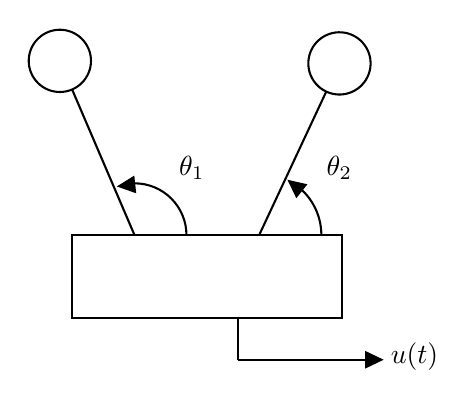
\begin{tikzpicture}[x=0.75pt,y=0.75pt,yscale=-1,xscale=1]
%uncomment if require: \path (0,300); %set diagram left start at 0, and has height of 300

%Shape: Rectangle [id:dp5552980078605938] 
\draw   (250,150) -- (380,150) -- (380,190) -- (250,190) -- cycle ;
%Straight Lines [id:da17705055918057389] 
\draw    (250,80) -- (280,150) ;
%Shape: Circle [id:dp397666828720904] 
\draw   (229,66) .. controls (229,57.72) and (235.72,51) .. (244,51) .. controls (252.28,51) and (259,57.72) .. (259,66) .. controls (259,74.28) and (252.28,81) .. (244,81) .. controls (235.72,81) and (229,74.28) .. (229,66) -- cycle ;
%Straight Lines [id:da7989833151597414] 
\draw    (372.26,81.01) -- (340,150) ;
%Shape: Circle [id:dp24273139832816637] 
\draw   (368.73,56.02) .. controls (374.91,50.51) and (384.39,51.05) .. (389.9,57.23) .. controls (395.42,63.41) and (394.88,72.89) .. (388.7,78.41) .. controls (382.52,83.92) and (373.03,83.38) .. (367.52,77.2) .. controls (362,71.02) and (362.54,61.54) .. (368.73,56.02) -- cycle ;
%Shape: Arc [id:dp43093366133446853] 
\draw  [draw opacity=0] (271.45,126.5) .. controls (274.12,125.53) and (277,125) .. (280,125) .. controls (293.81,125) and (305,136.19) .. (305,150) -- (280,150) -- cycle ; \draw    (274.32,125.65) .. controls (276.15,125.22) and (278.05,125) .. (280,125) .. controls (293.81,125) and (305,136.19) .. (305,150) ;  \draw [shift={(271.45,126.5)}, rotate = 353.84] [fill={rgb, 255:red, 0; green, 0; blue, 0 }  ][line width=0.08]  [draw opacity=0] (8.93,-4.29) -- (0,0) -- (8.93,4.29) -- cycle    ;
%Straight Lines [id:da7564650429680718] 
\draw    (330,210) -- (370.88,210) -- (397,210) ;
\draw [shift={(400,210)}, rotate = 180] [fill={rgb, 255:red, 0; green, 0; blue, 0 }  ][line width=0.08]  [draw opacity=0] (8.93,-4.29) -- (0,0) -- (8.93,4.29) -- cycle    ;
%Straight Lines [id:da9574484712831245] 
\draw    (330,190) -- (330,210) ;
%Shape: Arc [id:dp22387355547567533] 
\draw  [draw opacity=0] (353.62,123.26) .. controls (363.34,128.23) and (370,138.34) .. (370,150) -- (340,150) -- cycle ; \draw    (356.31,124.81) .. controls (364.55,130.16) and (370,139.44) .. (370,150) ;  \draw [shift={(353.62,123.26)}, rotate = 38.55] [fill={rgb, 255:red, 0; green, 0; blue, 0 }  ][line width=0.08]  [draw opacity=0] (8.93,-4.29) -- (0,0) -- (8.93,4.29) -- cycle    ;

% Text Node
\draw (300,110.4) node [anchor=north west][inner sep=0.75pt]    {$\theta _{1}$};
% Text Node
\draw (402,200.4) node [anchor=north west][inner sep=0.75pt]    {$u( t)$};
% Text Node
\draw (371,110.4) node [anchor=north west][inner sep=0.75pt]    {$\theta _{2}$};


\end{tikzpicture}
    
    \caption{Uncontrollable system example}
    \label{fig:uncontrollable}
\end{figure}
It is apparent that there is no choice of $\bm{u}$ that allows us to control both the pendulum on the left and the right simultaneously, because both have different starting conditions. We would like some mathematical rigor to understand the controllability of our system, however. Even better, we would like to develop this in a way that's independent of the controller design. This test will tell us if stabilizing control is possible at all.

The key idea is this: if we sent an impulse response through our system and it does not affect one or more of our states, then there is no possible way for us to control that state! Remember that we were able to construct the response of the generic function as an infinite sum of impulse functions. Given a generic impulse, if it has no interaction with a part of the state, how could we control that part? The fact of the matter is that we cannot, unless we made some physical alterations to how the system itself (mathematically, changing $A$ and $B$). With this argument in mind, we can come up with a more mathematical way to find if our system is controllable.

Let's start by considering a \textit{discrete} system, which is similar to the systems we've considered before. For this section, I'm going to replace $\Phi$ by $A$ for notational convenience. The details don't matter much anyways, since what follows isn't an exact proof. If you want a full proof, that is given in \autoref{Controllability proof}. While that is rigorous, I don't think it gives a good idea of what's going on unless you deeply understand the mathematics of the situation. We'll consider a discrete system which looks like the system we've seen before:
$$x_{n+1}=Ax_n+Bu_n$$
Consider sending the discrete time equivalent of an impulse $u_n=\delta(t)$ through our system at rest, where $x_n$ can be assumed to be a zero vector at the start. At the instant we send that impulse through the system, the response is going to be just the term associated with the input $u_n$. As a result, we would see that our state at the next time step, $x_{n+1}$, is going to be this term, $Bu_n$. We remember that for a $\delta$ input, this $u_n$ is simply $1$ in the Laplace domain.\endnote{In discrete time, we're not working in the Laplace domain, but in the $z$-domain. Just think of this discrete input as something which takes on a value if $1$ for the short interval of one discrete step. In leue of introducing many new concepts, I just use slightly incorrect language here. This `proof' isn't rigorous either, so it doesn't matter much if you're not a pedant.} Then, our first state is simply going to be the matrix $B$:
$$x_{n+1}=0A+B$$
Let's march forward a step in time, so that this $B$ vector is our new state, $x_n$. Our $u_n$ is now zero, since that delta function input only lasts for the first step in time. Plugging in to our equation, we see that $x_{n+1}=AB$, since we just multiply $A$ by our previous state. We'll continue this pattern on multiplying by $A$ at each future time, such that our state vector evolves like:
$$\mathcal{C}=\begin{bmatrix}
    B&AB&A^2B&A^3B&\cdots&A^{n-1}B
\end{bmatrix}$$
Once we reach the dimension of $A$ ($n\times n)$, it turns out that we don't get any more information from this matrix we've constructed. The reason is pretty simple -- this matrix can't have any more linearly independent columns after it exceeds the size of $A$. It is a simple fact of linear algebra. As a result, we only need to perform this multiplication to the point where we have $A^{n-1}$.\endnote{We may also use Cayley-Hamilton Theorem to show this fact. See \autoref{cayley hamilton} for more info.}

We've constructed this nice matrix which tells us what happens when we put a delta function through our system. If each of the elements of the state vector have been affected by this input, we'll expect them to appear in this matrix. 

We can devise a pretty simple test to see if any part of our state has made it into this matrix. We'll simply look at the \textit{rank} of this matrix. If any of our elements of the state vector weren't affected, the matrix will have a rank which is smaller than $n$. Using this condition, we have our final condition for controllability:
\begin{gather}
\color{boxBlue}\boxed{\color{black}\mathrm{rank}\left(\begin{bmatrix}
    B&AB&A^2B&\cdots&A^nB
\end{bmatrix}\right)}\\
\color{boxBlue}\text{Controllability Test}
\end{gather}
When the rank of the controllability matrix, $\mathcal{C}$, is the same as $n$, then the system is controllable. Mathematically, if $\mathrm{rank(}\mathcal{C})=n\Leftrightarrow\text{System is controllable}$.

Of course, I will reiterate that this `proof' was not exact. We did not show that this holds for the continuous time case, either (it does). If you want a more precise proof, that can be found in \autoref{Controllability proof}. The result holds nonetheless. With these ideas established, we can add a few other corollaries. For a controllable system:
\begin{itemize}
    \item It is possible to go from any one state, $x$, to another state $x'$ in the space $\mathbb{R}^n$ in an arbitrary time
    \item We can choose to place the eigenvalues of the system anywhere in $\mathbb{C}$.
\end{itemize}

\subsection{Controllers}

Now that we have developed an understanding of when a system is controllable, let's develop a typical form for a controller in the state space representation. Our typical controller acts on the state $\bm{x}$ and changes the eigenvalues of the system to change the stability characteristics. To see how this lends itself to changing the eigenvalues of the system, we can consider a simple controller of this form-- one which simply takes the current state, $\bm{x}$, multiplied by some constant matrix as its control input.

From this description, we have a control system where $\bm{u}=-K\bm{x}$. Upon plugging in $\bm{u}$, we have
$$\bm{\dot{x}}=A\bm{x}-BK\bm{x}$$
We can factor out $\bm{x}$, which returns our system to a very similar form to $\bm{\dot{x}}=A\bm{x}$:
$$\bm{\dot{x}}=(A-BK)\bm{x}$$
We can see that of $A-BK$ plays the role that $A$ does is the equation $\bm{\dot{x}}=A\bm{x}$. Thus, the eigenvalues of $A-BK$ tells us about the stability of the system under control. When the system is controllable, we can select $K$ in such a way to put the eigenvalues where we desire.

Upon seeing this, an obvious question arises. How should we pick $K$? In classical control, we used the root locus or the Bode plot to understand a good value for $K$. Here, our approach can be much more powerful. In fact, we can find an optimal $K$ if our system is linear -- more on that in the chapters to follow. Let's start with an approach that lets us put our poles wherever we would like them.

\textbf{Pole Placement}
One of the corollaries from our controllability theorem is that if our system is controllable, we may place the poles of the system anywhere in the complex plane. For an \gls{lti} system, a static gain matrix $K$ will be good enough to put the poles of the system into whatever location that we desire. Defining $\bar{A}=A-BK$, we have a known formula to place the poles, called \textit{Ackermann's formula}:
$$K=\begin{bmatrix}
    0&0&I
\end{bmatrix}{\mathcal{C}}^{-1}\Delta(\bar{A})$$
Here, $\mathcal{C}$ is the controllability matrix. We define $\Delta(s)$ as the polynomial with the desired pole locations . This polynomial is the characteristic equation for the system with the controller. We write:\endnote{We can show via the Cayley-Hamilton theorem that $\bar{A}=A-BK$ will satisfy it's own characteristic equation (this theorem is included in the controllability proof in \autoref{Controllability proof}).}
$$\Delta(s)\equiv\det(sI-(A-BK))=(s-p_1)(s-p_2)\cdots (s-p_n)$$
When we write it this way, we can prove that this type of controller will work for a system of any size (as long as it is controllable). However, it doesn't make the design process very intuitive. We will be better informed by an example.

\newpage
\begin{example}[Pole Placement]
Let's consider an open loop matrix which is initially unstable:
$$A=\begin{bmatrix}
0&1&0   \\0&0&1\\1&-2&2
\end{bmatrix}$$
All three eigenvalues of this system are unstable: $\lambda=1,\frac{1}{2}\pm\frac{\sqrt 3}{2}$. We will assume the standard canonical form for the $B$ matrix:
$$B=\begin{bmatrix}
    0&0&1
\end{bmatrix}^T$$
Since our control law is $u=-Kx$, we can directly find the matrix $A-BK$ now. Here, $K$ is the matrix:
$$K=\begin{bmatrix}
    K_1&K_2&K_3
\end{bmatrix}$$
And $A-BK$ is:
$$A-BK=\begin{bmatrix}
    0&1&0\\0&0&1\\1-K_1&-2-K_2&2-K_3
\end{bmatrix}$$
We can see the use of the controllable canonical form, as we can directly form the characteristic equation:
$$\Delta(s)=s^3-(2-K_3)s^2-(-2-K_2)s-(1-K_1)$$
Now, we can select desired poles for the system. Here, we will choose poles at $-2,-3$ and $-4$. The equation for those poles would be:
$$(s+2)(s+3)(s+4)=s^3+9s^2+26s+24$$
We now simply equate these two and solve for the values of $K$ to get our pole placement controller:
$$s^3-(2-K_3)s^2-(-2-K_2)s-(1-K_1)=s^3+9s^2+26s+24$$
We can solve $s^k$ term independently and find:
$$K=\begin{bmatrix}
    25&24&11
\end{bmatrix}$$
\end{example}
It is also easy to perform pole placement in MATLAB. Using the same system, we could define a pole placement controller as follows:
\begin{matlabscript}{Pole Placement Controller}
% set up the state matrix
A = [0 1 0;0 0 1;1 -2 2];
B = [0 0 1]';

% compute its eigenvalues
eig(A)

% check if it is controllable
rank(ctrb(A,B))

% place the eigenvalues
place(A,B,[-2,-3,-4])
\end{matlabscript}
This script produces the same output for $K$ as we found when we computed by hand. Note that the MATLAB function requires that all of the pole locations are distinct.


\section{Observability}
Observability is the other side of the coin. When we talk about a system being observable, we ask if we can determine the full state of the system from the outputs that we see. You'll notice that's a very similar question that we had a for a controllable system. As we already saw, the observability is the dual of the controllability problem. As a result, the two conditions will show striking similarities.

We start in much the same way as we did for the controllability condition. This time, we want to examine if it is possible to see a certain output. We'll do things in the discrete time domain again. The important new equation is that:
$$\bm{y}_n=C\bm{x}_n+D\bm{u}_n$$
For observation of a system, we can disregard the signal $u$. Since that is a signal that we are producing, it is obvious that we will be able to observe it. We are only concerned with the state $\bm{x}$ itself. This time, let's imagine that our system is in some initial configuration $\bm{x}_0$. We can imagine that some control input got it to that state, but for our purposes we will consider that after $\bm{x}_0$, no control is applied.\endnote{If we derive things in the more mathematical way, we can see that the control input can be incorperated. } Remember that we still have the state update equation:
$$\bm{x}_{n+1}=A\bm{x}_n$$
At the first time in our system, the output will be $C$ multiplied by the initial state $\bm{x}_0$:
$$\bm{y}_0=C\bm{x}_0$$
At the next step, $\bm{x}_1$ will be $A\bm{x}_0$ according to our state update equations. So our result is:
$$\bm{y}_1=CA\bm{x}_0$$
The pattern continues for further timesteps, so we end up getting:
$$\begin{bmatrix}
    C\\CA\\CA^2\\\vdots \\CA^{n-1}
\end{bmatrix}\bm{x}_0$$
At this point, we can divide out the initial state $\bm{x}_0$ and we are left with the observability condition. Again, we only need to go up to the size of a square matrix because we gain no other linearly independent information beyond that.

$$\mathcal{O}=\begin{bmatrix}
    C\\CA\\CA^2\\\vdots \\CA^{n-1}
\end{bmatrix}$$
As before, the condition for observability is that the rank of this matrix is the same as the size of the state, $n_x$. We can test the observability of a system in MATLAB using the commands:
\begin{matlabscript}{Observability}
A = [0 1;1 0];
C = [0 1];

obsv(A,C)
\end{matlabscript}

\section{Observers}

Designing an observer for a system is almost identical to designing a controller for a system. For an observer, we would like to estimate the true state of the system. Eventually, our estimate should be the same as the actual state of the system for a good observer. When the state is observable, we know that this can be done (just like a controller can eventually stabilize the system).

To start, we'll define our estimate of the system. This estimate, our `best guess' of the state, is given the notation $\bm{\hat{x}}$. If we know the dynamics of the system, our best guess should still evolve according to the $A$ and $B$ matrices like:
$$\bm{\dot{\hat{x}}}=A\bm{\hat{x}}+B\bm{u}$$
However, we want to incorporate the measurements of the system! To do that, we will include the following:
$$L(\bm{y}-C\bm{\hat{x}})$$
Here, $y-C\hat{x}$ tells us how much our measurement differed from what we expected to measure.\endnote{We will call this an innovation in the future.} Remember that $C$ will convert the state into the same format as a measurement, $\bm{y}$. Think about $L$ as the same as a control gain $K$. It determines what we want to do about the difference between our measurement and expectation. If they are far away from each other, we can push our estimate of $\bm{\hat{x}}$ in some direction to reduce the difference between our measurement and the expectation. In this way, we can incorporate the result of system measurements to help us estimate our state better. The full dynamics for our state estimate will then be:
$$\bm{\dot{\hat{x}}}=A\bm{\hat{x}}+B\bm{u}+L(\bm{y}-C\bm{\hat{x}})$$

Since we want the true state and the estimated state to eventually match, we'll define an error between them:
$$\bm{e}=\bm{x}-\bm{\hat{x}}$$
Now, we can reformulate the problem entirely in terms of the error:
$$\bm{\dot{x}}-\bm{\dot{\hat{x}}}=A\bm{x}+B\bm{u}-[A\bm{\hat{x}}+B\bm{u}+L(\bm{y}-C\bm{\hat{x}})]$$
Which simplifies to the following when we substitute $\bm{y}=C\bm{x}$:
$$\bm{\dot{e}}=A(\bm{x}-\bm{\hat{x}})-LC(\bm{x}-\bm{\hat{x}})$$
Which is of course:
$$\bm{\dot{e}}=A\bm{e}-LC\bm{e}=(A-LC)\bm{e}$$
After all that math, we come to the important conclusion that the observer will reach zero error when the eigenvalues of $A-LC$ are negative. Now, we have something very similar to the control criteria that we can use to create systems with good state estimates. When a system is observable, we can design an observer $L$ which will place the poles of the system wherever we desire. The process to do so is very similar to the design of a gain matrix $K$ using the pole placement technique.

\begin{example}[Observer Design]
Consider that we have a mass spring system where the observed quantity is the position of the system. We would like to estimate the full state including the velocity. The relevant quantities are:
$$\bm{x}=\begin{bmatrix}
    x&\dot{x}
\end{bmatrix}^T\quad A=\begin{bmatrix}
    0&1\\-1&0
\end{bmatrix}\quad C=\begin{bmatrix}
    1&0
\end{bmatrix}$$
We can easily see that the observability matrix has rank 2. We will design the observer with $L=\begin{bmatrix}
    L_1&L_2
\end{bmatrix}^T$, which is required for compatibility of sizes. This gives:
$$A-LC=\begin{bmatrix}
0&1-L_1\\-1&-L_2
\end{bmatrix}$$
We can find the eigenvalues of the system with $sI_2-(A-LC)$. The characteristic equation is given by the standard $2\times2$ determinant:
$$(sI-A+LC)=\begin{bmatrix}
    s&-1+L_1\\1&s+L_2
\end{bmatrix},\quad\Delta(s)=s^2+L_2s-L_1+1$$
We can set this equal to the desired poles. Let's choose $-3,-4$ to get:
$$s^2+L_2s-L_1+1=s^2+7s+12$$
Which yields $L=\begin{bmatrix}
-11&7
\end{bmatrix}^T$
    
\end{example}

\subsection{Controller and Observer Duality}
In the past examples we have seem very real symmetries between the design of controllers and observers. When we discussed the canonical forms, we found that the two were related by transposition and changes between the $B$ and $C$ matrices. For our benefit here, I've reproduced those equations:
\begin{gather}
A_\text{ctrb}=A_\text{obsv}^T\\
B_\text{ctrb}=C_\text{obsv}^T\\
C_\text{ctrb}=B_\text{obsv}^T\\
D_\text{ctrb}=D_\text{obsv}^T\\
\end{gather}
Now, we'll see how this duality can reproduce what we have seen in the past section. We already have a well formulated method for design of controllers, so we'll see if we can turn our observer problem into a controller problem. We'll start with the observer setup, and be explicit that these matrices are for the `obsv':
$$A_\text{obsv}-LC_\text{obsv}$$
We start by transposing the whole system:
$$(A_\text{obsv}-LC_\text{obsv})^T=A_\text{obsv}^T-C_\text{obsv}^TL^T$$
We can now make the appropriate substitutions for the problem. We will also define $L^T\equiv K$. We see that we recover the controller form:
$$A_\text{ctrb}-B_\text{ctrb}K$$
The result is simple, but pretty powerful. We can convert any observer problem into a controller problem using the \textit{dual} of the space where $(A,B,C,K)\rightarrow(A^T,C^T,B^T,L)$. Practically, we can use this in MATLAB to design an observer. Given a state space model $(A,B,C)$, we can find a pole placement observer $L$ via:
\begin{matlabscript}{}
L = (place(A',C',[-3,-4]))'
\end{matlabscript}


\section{Nonlinear State Spaces}
Most of the systems that we deal with in aerospace applications are nonlinear. As such, we need methods that allow us to understand the dynamics of nonlinear systems. Mostly, there are two main techniques that we use:
\begin{enumerate}
    \item Linearization of a nonlinear system around some equilibrium point
    \item A transformation to make the system linear / close to linear
\end{enumerate}

For this chapter, we'll mostly focus on the first approach. The second approach is explored in \autoref{part: advanced topics}. We'll use system linearization for many things, including the extended Kalman Filter and for control of nonlinear systems like the inverted pendulum (\autoref{chap:inverted pendulum}). System linearization is very powerful. The idea is very simple. Given a nonlinear state space or system dynamics, we take a first order Taylor series of the system in order to get a linearization of the system.

To begin, let's state what a general nonlinear state space model looks like:
\begin{gather}
\bm{\dot{x}}=f(\bm{x},\bm{u})\\
\bm{y}=h(\bm{x},\bm{u})
\end{gather}
These functions may take any form, so long as the they are only functions of the state. The defining attribute is that we must still be able to define the evolution of the state using just the knowledge of the state and control input.

\subsection{Linearization}
Linearization of systems gives us a method by which any high order function can be turned into a linear system. The idea is simply stated. We'll consider a non-linear function, $f(x)$. At a point $x^*$, the function looks like the value at the point $x^*$ plus it's first derivative at that point. This is equivalent to a first-order Taylor series:
$$f(x)\approx f(x^*)+f'(x^*)(x-x^*)$$
\begin{figure}
    \centering



\tikzset{every picture/.style={line width=0.75pt}} %set default line width to 0.75pt        

\begin{tikzpicture}[x=0.75pt,y=0.75pt,yscale=-1,xscale=1]
%uncomment if require: \path (0,300); %set diagram left start at 0, and has height of 300

%Curve Lines [id:da9284024876888896] 
\draw    (180,237.06) .. controls (321.58,293.28) and (391.01,18.42) .. (490.8,136.3) ;
%Straight Lines [id:da4830726652559222] 
\draw [color={rgb, 255:red, 218; green, 44; blue, 0 }  ,draw opacity=1 ][line width=1.5]  [dash pattern={on 5.63pt off 4.5pt}]  (338.71,175.56) -- (412.32,100) ;
\draw [shift={(338.71,175.56)}, rotate = 314.25] [color={rgb, 255:red, 218; green, 44; blue, 0 }  ,draw opacity=1 ][fill={rgb, 255:red, 218; green, 44; blue, 0 }  ,fill opacity=1 ][line width=1.5]      (0, 0) circle [x radius= 3.48, y radius= 3.48]   ;

% Text Node
\draw (348,175.4) node [anchor=north west][inner sep=0.75pt]  [color={rgb, 255:red, 218; green, 44; blue, 0 }  ,opacity=1 ]  {$f\left( x^{*}\right)$};
% Text Node
\draw (318,67.4) node [anchor=north west][inner sep=0.75pt]    {$f( x) \approx f\left( x^{*}\right) +f'( x^*)\left( x-x^{*}\right)$};
% Text Node
\draw (212,214.4) node [anchor=north west][inner sep=0.75pt]    {$f( x)$};


\end{tikzpicture}

    \caption{Linearization of a non-linear function}
    \label{fig:linearization}
\end{figure}

This is just a first order Taylor series approximation of a function. Obviously this approximation is only good when $x$ is in the vicinity of $x^*$. To make that assumption clear, we will denote $(x-x^*)$ as $\delta x$:
$$\delta x\equiv(x-x^*)$$
In this new notation, we can approximate $f(x)$ as:
$$f(x)\approx f(x^*)+f'(x^*)\delta x$$
Note that this $\delta$, which we call a perturbation, is different than the delta in the calculus of variations. For most applications they are not used at the same time, and it will be make clear if such cases arise. Note that we can apply the same technique of linearization to vector and matrix equations. The generalization is quite simple:
$$f(\bm{x})=f(\bm{x^*})+f'(\bm{x^*})\delta \bm{x}$$
Here, $f'$ is in general a Jacobian matrix given by $\frac{\partial f}{\partial \bm{x}}$.
\begin{example}[Sine Linearization]
We often see the following approximation used:
$$\sin(x)\approx x,\ x\approx0$$
We can use linearization to prove this fact. We'll apply the linearization formula and compute:
$$\sin(x)\approx\sin(x^*)+\cos(x^*)\delta x$$
Since we only apply this approximation for $x\approx0$, we'll linearize about that point. So, we substitute $x^*=0$ into the system and we find that:
$$\sin(x)\approx \sin(0)+\cos(0)\delta x$$
The result simplifies to $\sin(x)\approx \delta x$. Since we linearized about $x^*=0$, we have the simplification that:
$$\sin(x)\approx \delta x=(x-x^*)=x$$
Which is exactly the approximation we typically use. Notice that considering the approximation point to be 0 allowed us to remove the $\delta$ from our equation. We will often choose coordinates that let us do this.
\end{example}
\begin{exercise}[Matrix Linearization]\label{exer:matrix_linearization}
Compute the linearization of the following matrix system around the point $x^*=0$:
$$\bm{\dot{x}}=\begin{bmatrix}
x_2\\
-\sin(x_1)
\end{bmatrix}$$
\end{exercise}

Sometimes, rather than reducing a $n^\text{th}$ order equation into a set of $n$ first order equations and solving with a matrix equation, we can directly linearization on the higher order equation. Afterward, we may convert this into a linear state space model.

\begin{example}
We will linearize the following system about the point $x=0$ at equilibrium conditions:
$$\ddot{x}+x\dot{x}+3\sin(x)=u$$
If you write out all the steps of the linearization, you'll notice that we can treat $\delta x$ as similar to the derivative of $x$ when calculating the derivative. That is, it behaves similarly to the Gateaux derivative. Following that, we will find the linearization of the equation as:
$$\delta \ddot{x}+\dot{x}\delta{x}+x\delta\dot{x}+3\cos(x)\delta x=\delta u$$
Since we are considering equilibrium, any terms in $\dot{x}$ will go to zero. If the system is static, it's derivative must vanish! We then have:
$$\delta \ddot{x}+\cancel{\dot{x}\delta{x}}+\cancelto{0}{x\delta\dot{x}}+3\cancelto{1}{\cos(x)}\delta x = \delta \ddot{x}+3\delta x=\delta u$$
We can now reduce this second order linear equation to two first order equations:
\begin{gather}
\dot{x}_1=x_2\\
\dot{x}_2=-3x_1+u
\end{gather}
Which can be interpreted as the state space model:
$$\bm{\dot{x}}=\begin{bmatrix}
0&1\\-3&0
\end{bmatrix}\bm{x}+\begin{bmatrix}
    0\\1
\end{bmatrix}u$$
\end{example}

To recap, linearization is just an extension of the first order Taylor series of a function applied to state vectors. To linearize a system, we may take two approaches: either create a matrix representation first and then compute the Jacobian, or linearize the equations and then form a matrix equation.

\subsubsection{Interpreting Linearization}
By linearizing our systems, we are able to apply the analysis which we have discussed earlier in this chapter. However, we must be mindful of the limitations in doing so. Since we have only considered the first derivative of our system at a single point, linearization only gives us \textit{local} understanding of our system dynamics. Let's consider stability as an example. There are three scenarios for eigenvalues:
\begin{itemize}
    \item  $\text{Re}(\lambda)<0$ $\rightarrow$ the system is \textit{locally} asymptotically stable. We cannot say the entire system is stable.
    \item $\text{Re}(\lambda)>0$ $\rightarrow$ the system is locally unstable. The entire system cannot be globally stable, but other parts of the system may be locally stable.
    \item $\text{Re}(\lambda)=0$ $\rightarrow$ we cannot say anything about local stability. We require more than first order terms to determine stability.
\end{itemize}


\newpage
\printendnotes


\chapter{Optimal Control and LQR}\label{chap: optimal control}

So far, our study of control theory has given us several ways to create controllers. While each of these methods have proven useful for designing controllers which stabilize our system, none of these offer us any guarantee of optimal performance. Consider for example our study of the PID controller via the root locus method. We are easily able to design this controller to place the dominant poles of the system wherever we desire. If we were to ask: ``How much control effort does such a controller use when subjected to a step response'', the answer is not so simple. It is very hard to design such a controller with an explicit consideration for the amount of control. The same is true for lead-lag controllers, or almost any classical design methodology.

For some systems, the control effort is not much of a concern. Consider, however, a spacecraft which has limited fuel. In this case, we would be very interested in controlling the system and also minimizing the amount of fuel used! Many other systems are the same. In aerospace systems, there seems to be a huge variety of reasons to care about this: Power draw, actuator limits, part lifespan, etc. Needless to say, the control input is often as important as the stabilizing effects of the controller.

With our study of state space modeling, we have gained significant power compared to classical control theory. In the last chapter, we saw that we can place the poles of the system wherever we desire. However, we still lack a rigorous understanding of how we can minimize the control effort for such a system. Additionally, real world systems are complicated. Perhaps having our pole at $-1$ is trivial, but moving it to $-2$ requires so much additional work that it is not worth doing so. Pole placement gives us little ability to make such choices as a designer.

These stringent requirements make it almost essential to develop a framework for optimal control theory. This chapter will not discuss optimal control theory in the context of more general optimization problems. Those problems require more general tools, such as dynamic programming and Pontrayagin's maximum principle. Instead, we will focus on optimal control in the context of controlling linear systems. Leveraging our previous study of \gls{Lagrangian} and \gls{Hamiltonian} dynamics will allow us to study optimal control theory as a natural extension of these ideas in physics.  To begin our study, we will transition our knowledge of classical mechanics into the realm of optimal control.

\section{From Classical Mechanics to Optimal Control}
The ideas of optimal control are a direct extension of classical mechanics. In fact, optimal control is a generalization of the calculus of variations. As a result, it will be natural to begin our study this way. In optimal control theory, the \gls{Lagrangian} or \gls{Hamiltonian} of our system is not typically representative of the dynamics of the system itself (those properties belong in the $A,B,C,D$ matrices). Instead, these quantities are used to describe a \textit{cost functional}. Such a functional gives a description for how we want to assign a cost to each action in our system. In this formulation, we can place an explicit cost on high control in the system, or on large state values. Then, we use the same exact principles we used for a path of minimum action to find a solution which minimizes the cost subject to this new functional. Such a cost functional typically takes the following form:
$$J=\varphi[\bm{x}(\tau)]+\int_0^\tau L(\bm{x},\bm{u})dt$$
Here, $L$ is the familiar \gls{Lagrangian}, though it takes a different form than it did in classical control. The term $\varphi$ is known as a \textit{terminal cost}. It is some function of the final position of the system. If we care about where our system is after some time $\tau$, we can include a terminal cost to place a penalty on certain outcomes. Our explicit goal is to find inputs $\bm{u}$ into the system which minimize the value of this cost functional $J$. In the generic problem, the dynamics of our system can be any non-linear function of the state and the control:
$$\bm{\dot{x}}=f(\bm{x},\bm{u})$$
Since $L$ is no longer representing dynamics of the system, it is our job as designers to figure out what it should be. Since we will apply Euler-Lagrange to solve such a system, it's good for $L$ to be twice differentiable, scalar, and bounded from below.

\subsubsection{Differences between the Classical and Control Lagrangians}
Before we move on, it is important that we note the important differences between the \gls{Lagrangian} of classical physics and optimal control theory. The first difference is one we have already hinted at. The \gls{Lagrangian} in classical physics is required to take the form $L=T-U$. In the formalism of optimal control, we decide what $L$ should be to satisfy the particular requirements of our system. Additionally, optimal control problems are not necessarily a fixed boundary problem. In standard \gls{Lagrangian} physics, we had created our variation $\eta$ such that the endpoints were always vanishing. In optimal control, that is not necessarily the case. For example, we can consider an optimization problem where the objective is to minimize the time, in which case the terminal point $\bm{x}(\tau)$ is flexible.

The other important difference is how we handle the dynamics of the system. In classical mechanics, we used the \gls{Lagrangian} to find the equations of motion for a system. In control theory, it is acting as a functional with the state of the system as an input. However, we still require that the state evolves according to some specified dynamics.

One final distinction is that physicists typically prefer to work directly with the manifold structure of a space. When we defined covariant and contravariant indices for our vectors, we were implicitly doing this. For example, defining a generalized momentum conjugate as $p_i$ makes it implicit that this quantity is covariant (covector / 1-form). Engineers in control theory, likely because they often implement equations in computer software, prefer a notation closer to standard matrix equations. Vectors are canonically given as column vectors, and we transpose them when they are covariant quantities. Therefore, a control engineer would typically write the generalized momentum conjugate as:\endnote{Of course, a transposition like this only works in a Cartesian basis. Otherwise, a covector is not merely a transposition! Since we will be primarily concerned with linear systems, we can get away with this simplification. However, non-linear system dynamics will require us to think more carefully.}
$$p_i\rightarrow\bm{p}^T$$
\subsubsection{Lagrange Multipliers}
In standard \gls{Lagrangian} mechanics, we used the method of Lagrange multipliers in order to understand constraint forces in the system. We will use them in optimal control to enforce the dynamics of the system. The constraint is that the dynamical system must obey it's own equation:
$$\bm{\dot{x}}=f(\bm{x},\bm{u})\rightarrow f(\bm{x},\bm{u})-\bm{\dot{x}}=0$$
We will want to satisfy this constraint equation for each element in $\bm{x}$. Therefore, we define a column vector of Lagrange multipliers, given by $\bm{\lambda}$:
$$\bm{\lambda}=\begin{bmatrix}
    \lambda_1\\\lambda_2\\\vdots\\\lambda_n
\end{bmatrix}$$
Since the integrand is desired by be a scalar, we consider the inner product of $\bm{\lambda}$ with the constraint equation. As a physicist, we would be inclined to say that $\bm{\lambda}$ is a covariant quantity:
$$\bm{\lambda}^T[f(\bm{x},\bm{u})-\bm{\dot{x}}]$$
We can combine this with the original cost functional to come up with the following:
$$J=\varphi[\bm{x}(\tau)]+\int_0^\tau L(\bm{x},\bm{u})+\bm{\lambda}^T[f(\bm{x},\bm{u})-\bm{\dot{x}}]dt$$
The vector of Lagrange multipliers is often called the \textit{costate vector} in optimal control. It tells us how the dynamics of the system enter into the equations of motion.  To better understand the costate, it is necessary that we interpret it in a different way. We have already seen that it is a covariant quantity like the generalized momentum conjugate. Since our cost function is described by a \gls{Lagrangian}, it is natural that we might come up with a \gls{Hamiltonian} for our system in which the costate vector is the analog of the generalized momentum.

\subsubsection{The Control Hamiltonian}
Much like the control \gls{Lagrangian} is not exactly the same as the classical \gls{Lagrangian}, the control \gls{Hamiltonian} will be analogous but not exactly identical to the classical \gls{Hamiltonian}. To be precise, we will actually perform a Legendre-Fenchel transform rather than the standard Legendre transformation. This only transforms the equation with respect to the control input, $\bm{u}$ (therefore a transformation of $\bm{u}$ into $\bm{\lambda}$ under the transformation). Regardless of these small changes, we can still use the diverse set of tools developed in the context of classical mechanics in order to understand the \gls{Hamiltonian} in the context of controls.

In order to develop the control \gls{Hamiltonian}, we will consider a new mapping for our variables in the system. The state $\bm{x}$ corresponds to the generalized coordinates $\bm{q}$. The costate will map to the generalized momentum conjugate, $\bm{p}$. Let's remember that the standard Legendre transformation looks like:
$$\mathcal{H}=\bm{p}^T\bm{\dot{q}}-L$$
The analogy in control theory will not be exact. Since $\bm{\lambda}$ already appears in the \gls{Lagrangian}, it is not a separate coordinate in phase space like it was in classical mechanics. Additionally, we are going to flip the sign of $L$ in the Legendre transformation. We will define our state as analogous to the generalized coordinates, and the costate analogous to the generalized momentum. Then, we have the \textit{control Hamiltonian}:
$$\mathcal{H}(\bm{x},\bm{\lambda},\bm{u})=\bm{\lambda}^T\bm{\dot{x}}+L$$
Under this interpretation, the form of the costate equation becomes clear. It will simply satisfy one of Hamilton's equations of motion. We have:
\begin{gather}
\bm{\dot{\lambda}}=-\frac{\partial \mathcal{H}}{\partial \bm{x}}
\end{gather}
We also notice that the state satisfies its own equation:
$$\bm{\dot{x}}=\frac{\partial \mathcal{H}}{\partial \bm{\lambda}}=\bm{f}(\bm{x},\bm{u},t)$$
In the \gls{Hamiltonian} formulation, the adjoint has a more clear interpretation. It acts as the canonical momentum. In classical dynamics, the canonical momentum was one of the coordinates which `steered' the system through the phase space. More specifically, the momentum could be thought of as a measure of the `sensitivity' of a system to changes in position. We saw this in the Hamilton-Jacobi equations:
$$p_j=\frac{\partial S(\bm{q},\bm{\alpha},t)}{\partial q^j}$$
We see something similar in the control \gls{Hamiltonian}. Here, the classical action $S$ is replaced by the cost functional. Therefore, the costate will satisfy a similar equation. Instead of a classical action $S$, we will have a `cost-to-go', $V$. It describes how much effort we expect to expend from the current time $t$ until the end of the trajectory, $\tau$.\endnote{The derivation of this quantity comes from Bellman's dynamic programming principle, in which we solve the equations backwards in order to understand the optimal path. This is what allows us to understand how much cost is expected to be left at any point in time along the trajectory.} It is the exact control theoretic analog of the action, $S$. Thus, the costate satisfies the equation:
$$\lambda_j=\frac{\partial V(\bm{x},t)}{\partial x^j}$$
The interpretation of the costate follows in the same way that it does for the classical momentum. $\bm{\lambda}$ describes the resistance to changes in $V$ along certain directions in the state space. Since $V$ is a measure of cost-to-go, it requires a certain knowledge of how the system will behave in the future. We can therefore think of the costate as `planning' how the system needs to proceed in order to behave optimally.

With an understanding of the control theoretic versions of the \gls{Lagrangian} and \gls{Hamiltonian}, we are ready to solve one of the most fundamental problems in optimal control -- the linear quadratic regulator.

\section{Linear Quadratic Problems}

Linear quadratic problems are some of the few cases of optimal control problems which we can solve exactly with analytical solutions. Because these problems have quadratic costs, they have a very natural structure which is easy to solve. Remember that when we had a quadratic \gls{Hamiltonian}, we could easily utilize the symplectic structure to understand the solution. For that very same reason, linear state spaces with a quadratic cost functional give us problems which are analytically tractable. The most important idea in setting up linear quadratic problems is to understand the form of the cost functional. 

\subsection{The LQ Cost}
The \gls{lqr} and the associated problems are quite simple at the fundamental level. We create two weighting functions, $Q$ and $R$, which describe the weighting on the state and the weighting on the controller effort, respectively. $Q$ and $R$ determine the optimality conditions of the system.

\begin{example}[The simplest LQR]
    We can create a simple example to showcase \gls{lqr} control. Let's say you are shopping online for some M4 bolts that you need to build your new control system gadget. You look around and you find the following options as shown in \autoref{tab:LQR explained}:
\begin{table}[H]
    \centering
    \begin{tabular}{c|cl}
         Vendor&   Shipping Cost&Shipping Time\\\midrule
         McMasterCarr& 
     \$35&1 day\\
 Amazon& \$2&3 day\\
 AliExpress& Free&2 weeks
 \end{tabular}
    \caption{Shipping Time and Cost comparison}
    \label{tab:LQR explained}
\end{table}

Depending on your needs, one vendor may be better than another. If you really need to get the bolts by tomorrow, you'd be willing to pay really high shipping costs for McMasterCarr! Conversely, if want to minimize cost, AliExpress will be the optimal choice for you. Mathematically, we can represent this system with a `cost' function, $J$:
$$J=Q\cdot\mathrm{cost}+R\cdot\mathrm{time}$$
Depending on the selections of $Q$ and $R$, a different vendor will be the optimal one for you! If $Q$ is high, then there is a high cost associated with the shipping, and we should choose AliExpress to minimize this quantity.
\end{example}

The selection of $Q$ and $R$ is one of the most important things to keep in mind about \gls{lqr} control. Even if the controller is mathematically optimal, you still need to carefully consider the values of $Q$ and $R$ to make sure it meets your needs!

This is another reason to choose \gls{lqr}, as is that it allows for \gls{mimo} systems to be controlled more easily. In larger systems, it may be hard to fine tune the placement of the poles by hand, and changing the poles to guarantee good stability margins for a system can be quite non-intuitive. \Gls{lqr} controllers offer a solution to this dilemma by instead shifting the emphasis to selection of $Q$ and $R$ instead.

With this basic picture of the \gls{lqr} controller, we can begin formulating the controller in the more general context. We assign $Q$ to be a weighting on the state $\bm{x}$ and $R$ to be a weighting on the control input $\bm{u}$.

Since the values of $\bm{x}$ and $\bm{u}$ may take on negative values, it is best to take the square of their values in order to always get a positive result. Otherwise, negative values may give us a controller that has a negative cost. As such, we define the cost function in the following way:
$$J=\int_0^\infty(\bm{x}^TQ\bm{x}+\bm{u}^TR\bm{u})dt$$
We can recognize the quantities $\bm{x}^T\bm{x}$ and $\bm{u}^T\bm{u}$ as the matrix quadratic forms of these variables. Again, this is done to ensure that the cost function is always positive and the accumulated cost is real valued and positive (so long as $Q$ and $R$ and positive semi-definite matrices). Additionally, quadratic functions always have an absolute minimum value, which will guarantee that the \gls{lqr} controller can attain a minimization. Of course, this quadratic form is also useful for simplicity in finding a solution.

\subsection{Solving the LQR Problem}
Because we are able to formulate the \gls{lqr} problem in terms of cost functional which has a \gls{Lagrangian} and \gls{Hamiltonian} description, we can easily solve the problem using the methodologies we have already developed. For the \gls{lqr} problem, we will focus on a linear time-invariant state space of the following form:
\begin{gather}
\bm{\dot{x}}=A\bm{x}+B\bm{u}
\end{gather}
The measurements of the system are unimportant for the \gls{lqr} problem. We simply assume that the full state of the system is observable so that we can use full state feedback.

\subsubsection{The Symplectic Method}
Because we are able to formulate the \gls{lqr} problem in terms of cost functional which has a \gls{Hamiltonian}, we can exploit the symplectic structure of the problem in order to find the solution to the \gls{lqr} problem. By approaching the problem in this way, we are able to see that the \gls{lqr} problem has geometric structure which we can utilize. 

To begin, we describe the standard cost functional, which is the same as we had done for the \gls{Lagrangian} method:
$$J=\frac{1}{2}\int_{0}^\infty(\bm{x}^TQ\bm{x}+\bm{u}^TR\bm{u})dt$$
We remember that the control \gls{Hamiltonian} is defined as:
$$\mathcal{H}(\bm{x},\bm{\lambda},\bm{u})=\bm{\lambda}^T\bm{\dot{x}}+L$$
We can use the linear dynamics and the \gls{Lagrangian} to create the full \gls{Hamiltonian}:
$$\mathcal{H}(\bm{x},\bm{\lambda},\bm{u})=\bm{\lambda}^T(A\bm{x}+B\bm{u})+\frac{1}{2}\bm{x}^TQ\bm{x}+\frac{1}{2}\bm{u}^TR\bm{u}$$
To find the optimal control input for the system at each time, we take the partial derivative of $\mathcal{H}$ with respect to $\bm{u}$ and set it equal to zero. That will give an optimality condition for the control input:
$$\frac{\partial \mathcal{H}(\bm{x},\bm{\lambda},\bm{u})}{\partial \bm{u}}=\bm{\lambda}^TB+\bm{u}^TR=0$$
We can rearrange this equation to solve for $\bm{u}$, which is the optimal control, denoted $\bm{u}^*$. We simply need to solve the equation to find this value. We rely on the fact that $R$ is symmetric and invertible.
$$\bm{u}^TR=-\bm{\lambda}^TB\xrightarrow{R^{-1}}\bm{u}^T=-\bm{\lambda}^TBR^{-1}\xrightarrow{\text{transpose}}\bm{u}^*=-R^{-1}B^T\bm{\lambda}$$
We can substitute the optimal solution $\bm{u}^*$ back into the control \gls{Hamiltonian} now:
$$\mathcal{H}(\bm{x},\bm{\lambda})=\bm{\lambda}^T(A\bm{x}-BR^{-1}B^T\bm{\lambda})+\frac{1}{2}\bm{x}^TQ\bm{x}+\frac{1}{2}(-R^{-1}B^T\bm{\lambda})^TR(-R^{-1}B^T\bm{\lambda})$$


\section{Optimal Control Design Examples}

\newpage
\printendnotes



\chapter{Old LQR Chapter}\label{chap:linear quadratic}

All formulations of optimal control arise from the optimization of some cost function associated with the control problem. These controllers are often regulatory in nature, rather than being tracking algorithms. The most famous among these formulations is the \gls{lqr} controller, which will be the first optimal controller that is discussed here.

\section{LQR Control}
\Gls{lqr} control is a type of optimal control that is particularly well studied and used. Because of its wide use and simple interpretation, we should start our journey with optimal control here. \Gls{lqr} has come to use because it is easy to change the controller properties, it is quite intuitive, and it guarantees good phase and gain margins for the system. 

The \gls{lqr} control scheme is based on the principles of optimality that we have discussed in \autoref{part: energy mech}. The \gls{lqr} controller is the optimal controller for a linear system. This is the reason that the \gls{lqr} controller is called `linear'. The \gls{lqr} controller also employs a quadratic cost function, which we will see when we derive the mathematical model of the system.

\subsection{The LQ Cost}
The \gls{lqr} control scheme is quite simple at its base. It has two weighting functions, $Q$ and $R$, which describe the weighting on the state and the weighting on the controller effort, respectively. $Q$ and $R$ determine the optimality conditions of the system.

\begin{example}[The simplest LQR]
    We can create a simple example to showcase \gls{lqr} control. Let's say you are shopping online for some M4 bolts that you need to build your new control system gadget. You look around and you find the following options as shown in \autoref{tab:LQR explained}:
\begin{table}[H]
    \centering
    \begin{tabular}{c|cl}
         Vendor&   Shipping Cost&Shipping Time\\\midrule
         McMasterCarr& 
     \$35&1 day\\
 Amazon& \$2&3 day\\
 AliExpress& Free&2 weeks
 \end{tabular}
    \caption{Shipping Time and Cost comparison}
    \label{tab:LQR explained}
\end{table}

Depending on your needs, one vendor may be better than another. If you really need to get the bolts by tomorrow, you'd be willing to pay really high shipping costs for McMasterCarr! Conversely, if want to minimize cost, AliExpress will be the optimal choice for you. Mathematically, we can represent this system with a `cost' function, $J$:
$$J=Q\cdot\mathrm{cost}+R\cdot\mathrm{time}$$
Depending on the selections of $Q$ and $R$, a different vendor will be the optimal one for you! If $Q$ is high, then there is a high cost associated with the shipping, and we should choose AliExpress to minimize this quantity.
\end{example}

The selection of $Q$ and $R$ is one of the most important things to keep in mind about \gls{lqr} control. Even if the controller is mathematically optimal, you still need to carefully consider the values of $Q$ and $R$ to make sure it meets your needs!

This is another reason to choose \gls{lqr}, as is that it allows for \gls{mimo} systems to be controlled more easily. In larger systems, it may be hard to fine tune the placement of the poles by hand, and changing the poles to guarantee good stability margins for a system can be quite non-intuitive. \Gls{lqr} controllers offer a solution to this dilemma by instead shifting the emphasis to selection of $Q$ and $R$ instead.

With this basic picture of the \gls{lqr} controller, we can begin formulating the controller in the more general context. We assign $Q$ to be a weighting on the state $\bm{x}$ and $R$ to be a weighting on the control input $\bm{u}$.

Since the values of $\bm{x}$ and $\bm{u}$ may take on negative values, it is best to take the square of their values in order to always get a positive result. Otherwise, negative values may give us a controller that has a negative cost. As such, we define the cost function in the following way:
$$J=\int_0^\infty(\bm{x}^TQ\bm{x}+\bm{u}^TR\bm{u})dt$$
We can recognize the quantities $\bm{x}^T\bm{x}$ and $\bm{u}^T\bm{u}$ as the matrix quadratic forms of these variables. Again, this is done to ensure that the cost function is always positive and the accumulated cost is real valued and positive (so long as $Q$ and $R$ and positive semi-definite matrices). Additionally, quadratic functions always have an absolute minimum value, which will guarantee that the \gls{lqr} controller can attain a minimization.

\subsection{Using LQR Control}
Before we get to the derivation of the \gls{lqr} controller in the next section, I want to show the practical implementation of the \gls{lqr} controller for state space system. I will use a \gls{lqr} controller again in the development of the inverted pendulum in \autoref{chap:inverted pendulum}.

We start with a state space model of the system, which is of the form:
\begin{align}
\dot{\bm{x}}=A\bm{x}+B\bm{u}\\
\bm{y}=C\bm{x}+D\bm{u}
\end{align}
If we have a system that is stabilizable and has fully observable states, then we are free to readily apply \gls{lqr} control on the system. Since the \gls{lqr} controller relies on full state observability, $C$ is simply an identity matrix and $\bm{y}=\bm{x}$. That is, the output of the system is simply the same as the state vector. In this case, the controller is only dependent on $A$ and $B$, which dictate the controllability of the system.

In MATLAB, we can solve the \gls{lqr} problem by using the command "lqr(A,B,Q,R)". By default, this command will output a $1\times n$ vector $K$, which represents the control gain. The resulting control action is the product $u=-Kx$.

\begin{example}[Reaction Control LQR]
    A very good demonstration of the \gls{lqr} controller comes from reaction control systems. These systems often need to balance control input to minimize fuel loses while still maintaining high orientation accuracy. For this reason, LQR controllers are fairly well suited to this application. A small reaction control system using a \gls{lqr} controller is demonstrated here.
\end{example}


\subsection{Hamilton-Jacobi-Bellman Equation}
To begin the mathematical formulation of the problem, we consider a problem with (in the general case) non-linear dynamics. As we have seen before, non-linear dynamics can be represented in the form:
$$\dot{\bm{x}}=f(\bm{x},u,t),\quad \bm{x}(t_0)=\bm{x}_0$$
We can develop some notion of optimality in this system by considering a functional which defines a `cost' for the system. This cost is defined by the system \gls{Lagrangian}, as well as a terminal cost, denoted $S$. Altogether, the total cost function is:
$$J=\int_{t_0}^T{L(\bm{x}(\tau),u(\tau),\tau)d\tau}+S(\bm{x}(T))$$
This looks very similar to the problems we have previously encountered in the calculus of variations, but there is a term $u(\tau)$ that is present which we cannot appropriately solve for with our currently developed methods.

Of course, our goal in this problem is to find a solution that is optimal. To do so, we must define some notation for the optimal solution. 
The optimal control vector is defined as $u^*$. We define $u^*$ as the control vector that is necessary to minimize the functional over the whole range of $t_0\leq t\leq T$. When $u^*$ is applied on the non-linear system, it produces the optimal state vector, denoted $\bm{x}^*$.

To be clear, an optimal solution is one which minimizes the functional $J$. When an optimal control vector and state vector are present, the function $J$ attains a minimum value, which will be denoted $J^*$. Altogether, an optimal solution is of the form:
$$J^*=\int_{t_0}^T{L[(\bm{x}^*(\tau),u^*(\tau),\tau)d\tau}+S(\bm{x}^*(T))$$
In general, the value of the functional may be defined as:
$$J=J(\bm{x}(t_0),u(t),t_0)=
\int_{t_0}^T{L(\bm{x},u,\tau)d\tau}+S(\bm{x}(T))$$
Of course, we want to find the minimum value of this functional by selecting the appropriate function for $u$, which is the optimal control policy. This may be written:
$$J^*(\bm{x},t)=\min_{u[t_0,T]}\left[
\int_{t_0}^T{L(\bm{x},u,\tau)d\tau}+S(\bm{x}(T))\right]$$

The key insight is that we can break up the first integral into different domains, say from time $t_0$ to $t_1$ and $t_1$ to $T$ and the statement is still identical:
$$J^*(\bm{x},t)=\min_{u[t_0,t_1]}\min_{u[t_1,T]}\left[
\int_{t_0}^{t_1}{L(\bm{x},u,\tau)d\tau}+\int_{t_1}^{T}{L(\bm{x},u,\tau)d\tau}+S(\bm{x}(T))\right]$$

Any number of subdivisions is allowed, so long as the union of all the subintervals covers the whole domain of $[t_0,T]$. Notably, the future state of $\bm{x}(t)$ is only dependent on the initial condition $\bm{x}_0$  and the control input. The whole solution is uniquely determined by the initial conditions, control input and the dynamics of the system! You may think about this in the context of an ordinary differential equation. To define a trajectory, we must solve the differential equation generally (akin to understanding the dynamics) and then choose an initial condition to travel along. The control input is another factor in this problem which allows us to `steer' from an initial condition to an optimal path along the differential equation trajectory. 

The big takeaway is that to find the optimal control solution, we only need to consider the initial conditions value of $\bm{x}$ and the rest of the problem is dictated as a result of this. Take a minute to consider this, as this is the key idea behind understanding \gls{lqr}. Using this idea, we can reformat the cost function into two pieces -- an initial condition part, and the rest of the trajectory, both of which should be minimized.
$$J^*(\bm{x},t)=\min_{u[t_0,t_1]}\left[
\int_{t_0}^{t_1}{L(\bm{x},u,\tau)d\tau}+\min_{u[t_1,T]}\int_{t_1}^{T}{L(\bm{x},u,\tau)d\tau}+S(\bm{x}(T))\right]$$
This right hand side quantity:
$$\min_{u[t_1,T]}\int_{t_1}^{T}{L(\bm{x},u,\tau)d\tau}+S(\bm{x}(T))$$
can be replaced by $J^*(\bm{x}_1,t_1)$ for the reason previously discussed.
$$J^*(\bm{x},t)=\min_{u[t_0,t_1]}\left[
\int_{t_0}^{t_1}{L(\bm{x},u,\tau)d\tau}+J^*(\bm{x}_1,t_1)\right]$$
Now, we want to find the limiting behavior of the function as the difference between $t_0$ and $t_1$ becomes small. Applying this until $\Delta t$ is infinitesimal will give the optimal control policy, $u^*$. To do this, we redefine $t_1$ as $t_0+\Delta t$:
$$J^*(\bm{x},t)=\min_{u[t_0,t_0+\Delta t]}\left[
\int_{t_0}^{t_0+\Delta t}{L(\bm{x},u,\tau)d\tau}+J^*(\bm{x}(t_0+\Delta t),t+\Delta t)\right]$$

We may begin simplifying terms of the system to arrive at an answer. We consider the first integral:
$$\int_{t_0}^{t_0+\Delta t}{L(\bm{x},u,\tau)d\tau}$$
Considering the limiting behavior will be identical to the Riemann sum, the solution will look like the value at $L(\bm{x},u,\tau)$ multiplied by the integration length, $\Delta t$:
$$L(\bm{x},\bm{u},\tau)\Delta t$$
We can expand the term $J^*(\bm{x}(t_0+\Delta t),t_0+\Delta t)$ using a similar idea. We will only consider the first order derivative of $J^*$ as higher order terms are unimportant as $\Delta t\rightarrow0$. The process is shown graphically in \autoref{fig:J star}:\endnote{Note that this representation only shows the spatial dimension and not the temporal dimension as well for simplicity. For a full picture, imagine the time evolution of the $J^*$ function extending into 3-dimensional space. It then becomes apparent why we must also take the partial derivative with respect to time. The full picture is even more complex, as the state $\bm{x}$ is typically more than a single dimension}
\begin{figure}[ht]
    \centering

\tikzset{every picture/.style={line width=0.75pt}} %set default line width to 0.75pt        

\begin{tikzpicture}[x=0.75pt,y=0.75pt,yscale=-1,xscale=1]
%uncomment if require: \path (0,300); %set diagram left start at 0, and has height of 300

%Curve Lines [id:da8012449531711278] 
\draw    (160,217.06) .. controls (301.58,273.28) and (371.01,-1.58) .. (470.8,116.3) ;
%Straight Lines [id:da18205623463104004] 
\draw [color={rgb, 255:red, 218; green, 44; blue, 0 }  ,draw opacity=1 ] [dash pattern={on 4.5pt off 4.5pt}]  (318.71,155.56) -- (392.32,80) ;
\draw [shift={(355.52,117.78)}, rotate = 314.25] [color={rgb, 255:red, 218; green, 44; blue, 0 }  ,draw opacity=1 ][fill={rgb, 255:red, 218; green, 44; blue, 0 }  ,fill opacity=1 ][line width=0.75]      (0, 0) circle [x radius= 2.01, y radius= 2.01]   ;
\draw [shift={(318.71,155.56)}, rotate = 314.25] [color={rgb, 255:red, 218; green, 44; blue, 0 }  ,draw opacity=1 ][fill={rgb, 255:red, 218; green, 44; blue, 0 }  ,fill opacity=1 ][line width=0.75]      (0, 0) circle [x radius= 2.01, y radius= 2.01]   ;
%Straight Lines [id:da9534125190612921] 
\draw [color={rgb, 255:red, 218; green, 44; blue, 0 }  ,draw opacity=1 ]   (318.71,170.68) -- (352.52,170.68) ;
\draw [shift={(355.52,170.68)}, rotate = 180] [fill={rgb, 255:red, 218; green, 44; blue, 0 }  ,fill opacity=1 ][line width=0.08]  [draw opacity=0] (5.36,-2.57) -- (0,0) -- (5.36,2.57) -- cycle    ;

% Text Node
\draw (480.9,102.88) node [anchor=north west][inner sep=0.75pt]    {$J^{*}$};
% Text Node
\draw (337.11,174.08) node [anchor=north] [inner sep=0.75pt]  [color={rgb, 255:red, 218; green, 44; blue, 0 }  ,opacity=1 ]  {$\Delta x$};
% Text Node
\draw (282,142.4) node [anchor=north] [inner sep=0.75pt]  [font=\small,color={rgb, 255:red, 218; green, 44; blue, 0 }  ,opacity=1 ]  {$J^{*}( x,t_{0})$};
% Text Node
\draw (350.5,61.4) node [anchor=north] [inner sep=0.75pt]  [font=\small,color={rgb, 255:red, 218; green, 44; blue, 0 }  ,opacity=1 ]  {$\frac{\partial J^{*}( x,t_{0})}{\partial x}$};


\end{tikzpicture}
    
    \caption{Taylor Expansion of $J^*$}
    \label{fig:J star}
\end{figure}

First, we consider the value at the current state $(\bm{x},t_0)$, which can simply be written:
$$J^*(\bm{x},t_0)$$
Next, we consider the spatial and time derivatives of $J^*$, which will allow us to compute the new value after a shift of $\Delta t$. First considering the derivative with respect to time:
$$\frac{\partial J^*(\bm{x},t_0)}{\partial t}$$
This must be multiplied by the time delta to give the change over the course of $\Delta t$:
$$\frac{\partial J^*(\bm{x},t_0)}{\partial t}\Delta t$$
The derivative with respect to $\bm{x}$ is more complicated, since $\bm{x}$ is a vector of size $n \times 1$. The gradient operator is typically also a column vector of size $n\times1$, so it must be transposed to be compatible with matrix multiplication by $\bm{x}$. The first order value is thus given by:
$$\left(\frac{\partial J^*(\bm{x},t_0)}{\partial \bm{x}}\right)^T\Delta \bm{x}$$
Putting all of the pieces together, we have:
$$J^*(\bm{x},t_0)=\min_{u[t_0,t_0+\Delta t]}\left[L(\bm{x},u,\tau)\Delta t+J^*(\bm{x},t_0)+\left(\frac{\partial J^*(\bm{x},t_0)}{\partial \bm{x}}\right)^T\Delta \bm{x}+\frac{\partial J^*(\bm{x},t_0)}{\partial t}\Delta t\right]$$
This is a considerable simplification, as there are no longer any integrals present. There is a $J^*(\bm{x},t_0)$ present on both sides of the equation, so it can be subtracted. Finally, $\Delta t$ can be divided through the equation.
$$0=\min_{u[t_0,t_0+\Delta t]}\left[L(\bm{x},u,\tau)+\left(\frac{\partial J^*(\bm{x},t_0)}{\partial \bm{x}}\right)^T\frac{\Delta \bm{x}}{\Delta t}+\frac{\partial J^*(\bm{x},t_0)}{\partial t}\right]$$
At this point, we may perform a Legendre transform to make this equation amenable to further changes. Such a transformation will allow us to effectively remove the derivative and express it in terms of a Hamiltonian!

% use the 

\subsection{The Algebraic Riccati Equation}
At this point, we have encountered a quadratic matrix equation. This equation is quite famous, and is known as the \gls{are}. 



\section{LQI Control}

Throw an integral on there for tracking things




\section{Robustness}
Uncertain parameters in MATLAB, basic synthesis of Hinf and Mu controllers

\section{Other Optimal Control Problems}

The \gls{lqr} controller is one case where the optimal control problem has an analytical solution. Sometimes the solution to this equation must be evaluated numerically, but there still exists a closed form solution to the problem. However, in the more general case of the optimal controllers, there is not always a closed form solution to the minimization of the functional. 

\subsection{Gradient Descent}

\subsection{Stochastic Methods}


\section{Optimal Control Design Examples}

\newpage
\printendnotes



% \chapter{Preliminary Mathematics for Optimal Estimation}
\chapter{Introduction to Optimal Estimation}\label{chap:intro optimal est}
The introduction of state space methods has given us a taste for modern control theory. However, the next few topics that we want to cover in modern estimation and control are going to require a fair bit of mathematical tools. There is an assortment of tools that we will require, most of them coming from more advanced linear algebra. Instead of interrupting every few pages to introduce new mathematics, I will consolidate most of the core ideas into this chapter so we can focus on the control theory in the following chapters. In this chapter, there will be three core topics: least squares estimation, probability theory, and Hilbert spaces. All three of these will turn out to be intimately connected and introduce us to many important ideas.

The connection between all of these ideas has to do with the concept of \textit{optimality}. Ultimately, we don't just want to make controllers and observers with whatever gains \textit{seem} right. While such an approach works for some problems, we often want to ensure that the amount of control that we apply is limited or that we don't consume too many valuable resources to reach an end condition. These are all ways of saying that desire optimality. Doing so will elevate our control techniques, but will require a significant development of mathematics.


\subsubsection{What is Optimality?}
Before we get into any mathematical analysis, I should explain exactly what is meant by optimality. We have seen already many examples of what we may consider `optimal' behaviors. Consider the Brachistochrone curve in \autoref{ex:brachistrochrone}. In that example, we found an `optimal' condition which yielded a minimum time. We then extended this concept of least action more generally in our consideration of Lagrangian and Hamiltonian dynamics. From these various systems, we can see that what we consider an `optimal' solution to a problem may vary quite a bit, but our underlying principle of functional minimization has always been present.

When we discuss control systems, our idea of optimality is again somewhat distinct from our previous discussions. In optimal control, our goal is to find a solution that is optimal in regards to \textit{some objective function}. Our choice of a objective function, then, will change our solution and what we actually mean when we say our solution is \textit{optimal}. Part of our consideration is in choosing a good objective for our problem!

There is another distinct difference from our earlier problems. In those problems, we relied purely on the dynamics of a system to guide our optimization. That will be part of the story, but we will have much more control with the addition of an input $u$ into the system. This gives us much more power. The result is that we need to extend our ideas from the calculus of variations into a more broad theory known as optimal control. The incorperation of control into the problem means that we need to decide the optimal action to take at every step in addition to knowing the system dynamics.

To start this journey, we will first consider the topic of optimal estimation. It is slightly easier to grasp than optimal control, but the concepts will ultimately be deeply linked. We'll start at humble beginnings, with least squares estimation. Surprisingly and somewhat serendipitously, this simple start will guide us all the way to the Kalman filter and LQR controllers which are the cornerstone of optimal control. 


\section{Least Squares Estimation}\label{sec:least squares}
To start our discussion of optimality, we should first consider a quite simple case of optimality, which is the case of producing a least squares estimate. Least squares estimation is a deterministic method, but it will introduce techniques relevant the realm of optimal estimation.

Before we begin, it is best to discuss the players in the linear least squares estimation problem: $\bm{y}$, $H$, and $\bm{x}$. The variable $\bm{y}$ represents a collection of measurements, $\bm{x}$ a collection of states, and $H$ a mapping between the two. We can use these together to form the following equation:
$$\bm{y}=H\bm{x}$$
It is often the case that the measurements, $\bm{y}$ are not the same size as the vector $\bm{x}$. If we consider $\bm{y}\in\mathbb{R}^m$ and $\bm{x}\in\mathbb{R}^n$,  $H$ is a matrix which maps from $\mathbb{R}^m$ to $\mathbb{R}^n$. This system is representative of a general linear system of equations, which are all scalars equations of the form:
$$y=mx+b$$
Of course, real systems are not always perfectly linear, so the equation in reality look something like:
$$\bm{y}=H\bm{x}+e$$
Where $e$ is an error term describing how the measurements vary from the perfect linear fit. The goal of the least squares estimation is to find the value of $\bm{x}$ that best fits the measurements of the system and therefore minimizes $e$. The statement of this problem is fairly straightforward. Given $\bm{y}$, we desire a solution $H\bm{x}$ which minimizes their difference, $e$. We formulate this as:
$$\left\|\bm{y}-H\bm{x}_{opt}\right\|\leq\|\bm{y}-H\bm{x}\|\quad \forall \bm{x} \in \mathbb{C}^n$$
That is, we seek a solution for which the norm of the quantity $\bm{y}-H\bm{x}_{opt}$ cannot be made smaller by any other selection of $\bm{x}$. Stated another way, the problem is to find the minimization:
$$d=\min{\|\bm{y}-H\bm{x}\|:\bm{x} \in \mathbb{C}^n}$$
I should note here that in this problem, the values of $\bm{y}$ and $H$ are known, we simply want to find a value of $\bm{x}$ that results in a minimization of the system.

Students of linear algebra may think this problem is quite easy to solve at first glance. The minimization will just be the solution that exists when solving the equation:
$$\bm{y}=H\bm{x}$$
To find $\bm{x}$, we simply left multiply both sides of the equation of $A^{-1}$to get:
$$H^{-1}\bm{y}=\bm{x}$$
This is a classical result in linear algebra, but it is in fact not the solution we are seeking here! This solution will only hold in the case that $H$ is a square, invertible matrix, which is not the case in many of the problems that we want to analyze. As a result, we need to construct a more general method for finding the minimization of the equation.\footnote{Some information may be found in the video lecture series found at \cite{brunton_singular_nodate}.}

\subsubsection{The Least Squares Method}
Since we are not assuming square matrices, it is good to define the dimensions of each vector exactly. We consider $\bm{y}$ a column vector of dimension $m\times1$. We have previously stated that $\bm{x}$ is an $n\times1$ vector. To match the dimensions of $\bm{y}$, $H$ must be of dimension $m\times n$.

Since the vectors we have defined can have any size, there are three possible cases. When $m>n$, $H$ is a `tall' matrix. In the case of a tall matrix, the dimension of $\bm{y}$ is greater than the dimension of $\bm{x}$. In this case, there is no linear combination of $\bm{x}$ that can determine $\bm{y}$ fully. The best we can do is choose a value of $\bm{x}$ that gets us as close as possible. This is the case known as the \textit{overdetermined} case. This case is the typical least squares problem -- there are lots of data points, and we want to find a straight line that is as close as possible to representing their behavior.

On the opposite end, when $m<n$, $H$ is a `short' matrix. In this case, the exact opposite is true. There are many possible combinations of $\bm{x}$ that give $\bm{y}$, so an infinite number of solutions exist. This case is called the \textit{underdetermined} case. You may intuitive think of this as trying to fit a line to a single point. There are an infinite number of lines passing through that point, so the line is underdetermined!

Of course, there is the case where $m=n$ which is heavily studied in linear algebra classes. Readers should already be familiar with these solutions and how they relate to the above cases. Keeping with the analogy, this case corresponds to fitting a line to two points. There is a unique solution.

We can put aside the two different cases briefly while we determine the solution to our minimization problem. We can see from the matrix multiplication that the result of $\bm{y}-H\bm{x}$ is an $m\times1$ vector. To minimize this, we need to first convert this quantity to a scalar value. Of course, we can do that with the inner product, defining our scalar value as:
\begin{equation}\label{eq:least squares start}
    J=(\bm{y}-H\bm{x})^T(\bm{y}-H\bm{x})
\end{equation}
From here, the minimization is simply an application of calculus. We define the minimization as the point where the gradient of $J$ with respect to $\bm{x}$ is zero, or:
$$\frac{\partial J}{\partial \bm{x}}=0$$
We can apply this expression to the right hand side of the equation:
$$\frac{\partial}{\partial \bm{x}}\left[(\bm{y}-H\bm{x})^T(\bm{y}-H\bm{x})\right]=0$$
The transpose can first be expanded by the usual rule that $(AB)^T=B^TA^T$:
$$\frac{\partial}{\partial \bm{x}}\left[(\bm{y}^T-\bm{x}^TH^T)(\bm{y}-H\bm{x})\right]=0$$
Multiplying out the terms:
$$\frac{\partial}{\partial \bm{x}}\left[\bm{y}^T\bm{y}-\bm{y}^TH\bm{x}-\bm{x}^TH^T\bm{y}+\bm{x}^TH^TH\bm{x}\right]=0$$
We can notice that the middle terms, $\bm{y}^TH\bm{x}$ and $\bm{x}^TH^T\bm{y}$ are transpositions of each other. Since these terms are scalar (you can show this quite easily by analyzing their dimensions), the transposition operation means these terms are identical. As such, another simplification can be made by combining these terms.
$$\frac{\partial}{\partial \bm{x}}\left[\bm{y}^T\bm{y}-2\bm{x}^TH^T\bm{y}+\bm{x}^TH^TH\bm{x}\right]=0$$
You should notice that this form looks quite similar to the expansion of $(ax+b)^2$, and that is no coincidence! In fact, we call such terms quadratic. The form of $\bm{y}^T\bm{y}$ is in fact a matrix equivalent to $y^2$. The fact that this is quadratic is why we call this least `squares' estimation.

Our next step is to evaluate the partial derivative, which is quite similar to the standard methods in multivariate calculus. Since we can consider expressions such at $\bm{x}^T\bm{x}$ to be quadratic, its derivative is given by $2\bm{x}$. More rigorous derivations of this fact can be found, but the result holds nonetheless. Finally, we can perform the computation to get:
$$-2H^T\bm{y}+2H^TH\bm{x}=0$$
Which can be rearranged to:
$$H^TH\bm{x}=H^T\bm{y}$$
Solving for $\bm{x}$, we arrive at the final result:
$$\bm{\hat{x}}=(H^TH)^{-1}H^T\bm{y}$$
A `$\hat{\ \ \ }$' is added to $\bm{x}$ to denote that this value of $\bm{x}$ is not exact, but rather the best estimate of the value of $\bm{x}$ that can be attained from the system. 

The term $(H^TH)^{-1}H^T$ is the \textit{\gls{pseudoinverse}} of $H$, since it effectively does the same as $H^{-1}$ did in the case of the square matrix. One thing to note is that we could have either chosen $\bm{y}^TH\bm{x}$ or $\bm{x}^TH^T\bm{y}$ as the middle term, since both were identical scalars. Choosing one over the other changes the answer slightly. This is related to the underdetermined vs overdetermined case, which have slightly different \glspl{pseudoinverse}! The two cases of the \glspl{pseudoinverse} are shown for a general matrix $A$:

$$\begin{array}{rc}
     \mathrm{underdetermined:} & A^\#=A^T(AA^T)^{-1} \\
     \mathrm{overdetermined:} & A^\#=(A^TA)^{-1}A^T
\end{array}$$
\begin{exercise}[Pseudoinversion Immersion]
    It can be shown that these \glspl{pseudoinverse} are identical to the standard matrix inverse in the case of an invertible square matrix. You may consider the property that $(AB)^{-1}=B^{-1}A^{-1}$ to show this. 
\end{exercise}
Least squares estimation has given us some of the mathematical tools that we will need when considering optimal estimation in the more general sense.

Before we continue, lets stop briefly to consider the results of the least squares estimation. By considering the smallest inner product, we are effectively minimizing the 2-norm of the system. Along the way, we found that this corresponded to a quadratic matrix quantity.

We considered kinetic energy as one of the prototypical examples of a quadratic system. In fact, this analogy with kinetic energy is quite apt, as it turns out that minimizing the 2-norm corresponds to minimization of the energy! As we dive further into optimal estimation and control, this will be an important concept to keep in mind. Also remember that the Hamilton-Jacobi equations had exact solutions when the equation was quadratic. Thus, the quadratic form of these equations will turn out to be useful again in the future.

\subsection{Least Squares Estimation for State Spaces}
Understanding the least squares estimation problem in the context of state space modeling will get us one step closer to understanding optimal estimation as a whole.\footnote{The information in this section is adapted from the argument in \cite{kamen_introduction_1999}.} Let's consider our state space of the standard discrete time form:
\begin{gather}
\bm{x}_{n+1}=\Phi \bm{x}_n\\
\bm{y}_n=H\bm{x}_n+\bm{v}_n
\end{gather}
Notice that we are not considering the addition of a control signal $\bm{u}$ for now. We will consider adding that in later. We also assume that our modeling of the state update is perfect. However, our measurements are polluted by a noise $\bm{v}_n$. This is equivalent to the error $e$ we discussed in the previous section. To perform least squares estimation, we need to know the time history of the system vector. We can express this as:
$$\begin{bmatrix}
    y_1\\y_2\\\vdots\\y_n
\end{bmatrix}=\begin{bmatrix}
    Hx_1\\Hx_2\\\vdots\\Hx_n
\end{bmatrix}+\begin{bmatrix}
    v_1\\v_2\\\vdots\\v_n
\end{bmatrix}$$
However, we have information about how the state $\bm{x}$ evolves. Therefore, we can find any state $\bm{x}_j$ as:
$$\bm{x}_j=\Phi^{-n+j}\bm{x}_n$$
We can then express the time history purely in terms of the current state:
$$\begin{bmatrix}
    y_1\\y_2\\\vdots\\y_n
\end{bmatrix}=\underbrace{\begin{bmatrix}
    H\Phi^{-n+1}\\H\Phi^{-n+2}\\\vdots\\H
\end{bmatrix}}_{\mathcal{H}_n}\bm{x}_n+\begin{bmatrix}
    v_1\\v_2\\\vdots\\v_n
\end{bmatrix}$$

We may call this quantity $\mathcal{H}_n$ as the `history' vector for the state. We notice that this is exactly the same as the standard least squares estimation problem now, and we may find the estimate of $\bm{x}_n$ as:
\begin{equation}\label{eq:least squares xhat}
\bm{\hat{x}}_n=\left(\mathcal{H}_n^T\mathcal{H}_n\right)^{-1}\mathcal{H}_n^T\bm{y}_n
\end{equation}

Notice that this vector $\mathcal{H}_n$ is closely related to the observability matrix. The transformation to the observability matrix $\mathcal{O}$ is simple:
$$\mathcal{O}=\mathcal{H}_n\Phi^{1-n}$$
Thus we can also relate the estimate of the state to the observability matrix for the system:
\begin{equation}\label{eq:xhat observe}
\bm{\hat{x}}_n=\Phi^{n-1}\left({\mathcal{O}}_n^T\mathcal{O}_n\right)^{-1}\mathcal{O}_n^T\bm{y}_n
\end{equation}

\subsubsection{Estimation Error}
While least squares estimation does give a way to find an estimate for our state, it is not the optimal method. We can see this via a fairly simple argument. As we saw before, the error in estimation is given by the following:
$$\bm{\tilde{x}}_n=\bm{x}_n-\bm{\hat{x}}_n$$
We've already seen that the measurement equation is the following:
$$\bm{y}_n=H\bm{x}_n+\bm{v}_n=\mathcal{O}_n\Phi^{1-n}\bm{x}_n+\bm{v}_n$$
We can plug this result back into our equation for $\bm{\hat{x}}_n$ in \autoref{eq:xhat observe}:
\begin{equation}
\bm{\hat{x}}_n=\Phi^{n-1}\left({\mathcal{O}}_n^T\mathcal{O}_n\right)^{-1}\mathcal{O}_n^T(\mathcal{O}_n\Phi^{1-n}\bm{x}_n+\bm{v}_n)
\end{equation}
The reader should check that the terms of this equation cancel out quite nicely and leave us with the following:
\begin{equation}
\bm{\hat{x}}_n=\bm{x}_n+\Phi^{n-1}\left({\mathcal{O}}_n^T\mathcal{O}_n\right)^{-1}\mathcal{O}^T_n\bm{v}_n
\end{equation}
When we take the error, the first term in $\bm{x}_n$ simply gets canceled and we are left with:
$$\bm{\tilde{x}}_n=-\Phi^{n-1}\left({\mathcal{O}}_n^T\mathcal{O}_n\right)^{-1}\mathcal{O}^T_n\bm{v}_n$$
The result is obvious. The error in the estimation depends directly on the noise input to the system. Because this input is noise, we cannot directly quantify it. However, it gives us a clue that the deterministic least squares algorithm is not the optimal estimate. If we are able to quantify $\bm{v}_n$ \textit{statistically}, we can improve our estimate on average and lower the error in the system. It is for that reason that we have to study statistics in order to develop the optimal estimator.

\section{Some Preliminary Statistics}

To understand the Kalman Filter, we ultimately need to understand some basic statistics. Estimators are founded on the assumption that there is some noise in our system. Naturally, noise is a signal that cannot be quantitatively analyzed directly (otherwise it wouldn't be noise, we would call it something else). Noise comes from many sources, be they thermal, conversion processes, or of another origin. For many reasons, modeling noise in real time systems can either be challenging or literally impossible.\endnote{Consider, for example, a system which is quantum mechanical in nature. The system is stochastic and nature and there is no way around that.} To combat this, we add noise to our model and develop mathematics and control systems that can deal with this noise. We can quantify such randomness in the form of a \textit{random variable}.

\begin{definition}[random variable]
A  variable whose values are random but whose statistical distribution is known.
\end{definition}

The use of random variables in our systems to model noise allows us to apply the toolset of probability and statistics to analyze systems. Statistics has many tools to analyze systems of random variables which will be very useful in the development of the optimal estimator. To understand the mathematics of optimal estimators, we need to briefly discuss some of the statistical methods that are used.

The reader has likely seen many of these statistical ideas, but they may not have been presented in the case of continuous variables. In such cases, it may be good to try and show how you can recover the discrete case from what is shown here!

\subsection{Probability Distributions}

From our definition of a random variable, we know that it's statistical distribution is known or can be approximated. As a result, we'll use this statistical distribution to ascertain information about random quantities. In this way, we can develop information that will allow us to create better estimators even when our system has inherit noise. In the study of optimal estimation, knowing the probability distribution of noise parameters will allow us to make better estimations.

\subsubsection{Probability Density Function}
The first quantity that we must define is the \gls{pdf}. This is a function that tells us how likely a variable is to take on a certain value. It's easiest to start with the discrete case to understand probability density. 

\begin{example}[Dice Probability]
Let's consider a $6$-sided dice. We know that each number has a probability of $1/6$. Our probability density function will be:
$$p_X(x)=1/6,\quad\{x\in\mathbb{Z}|1\le x\le 6\}$$
The notation might seem kind of overkill for this example, but it should be simple to parse: The probability for any value of $x$ on the interval $1-6$ is $1/6$.
\end{example}

When we move to the continuous case, we no longer have a probability $p_X(x)$ for the variable. We instead have a \textit{density} associated with each value of $x$ in the real numbers (or some subset of the real numbers):
$$f_X(x),\quad x\in\mathbb{R}$$
Before we move on, let's talk about the notation. A capital letter, like $X$, is a random variable. This random variable can take on values $x$, which are a random selection from the distribution. The random variable $X$ though, is something that we do know. With the probability density function, it is important that it represents a real probability. There are two conditions that $f_X(x)$ has to satisfy to be a real probability density:

$$f_X(x)\ge 0 \  \forall x$$
$$\int_{-\infty}^\infty{f_X(x)}=1
$$

These conditions should be obvious. An event cannot have a negative probability of occuring and the total probability of all events must be $100\%$. That's about all there is to it. As long as the a function satisfies these criteria, it could describe the probability density of a random variable. \endnote{I should note that this continuous density function is more general than the discrete variable counterpart. We can describe a discrete variable using the continuous function if $f_X(x)$ takes the form of a Dirac-delta or multiple Dirac-delta functions.}

\begin{example}
Let's consider a situation in which we have a continuous random variable in our system which describes the thrust output of a reaction control thruster. We expect that this thrust could be anywhere between 50 and 60N with uniform probability. We would like to model the \gls{pdf} of the function to use later. We can describe the situation using a piecewise function:
$$f_X(x)=\begin{cases}
a&50<x<60\\
0&\text{else}
\end{cases}$$
To make this a proper \gls{pdf}, we need to find the appropriate value of $a$ which leads to a total probability of 1. This is pretty simple, we simply integrate the constant $a$ over the interval from 50 to 60:
$$\int_{50}^{60}adx=1$$
This leads us to find that $a=1/10$. We thus have the final \gls{pdf} for the system:
$$f_X(x)=\begin{cases}
\frac{1}{10}&50<x<60\\
0&\text{else}
\end{cases}$$
\end{example}

\subsubsection{Cumulative Density Function}
Sometimes we like to come up with a cumulative function which tells us the probability that a random variable, $X$, will have a value less than $x$. This is otherwise written:
$$F(x)=\Pr(X\leq x)$$
We can find this by integrating the probability density up to the point $x$:

$$F(x)=\int_{-\infty}^x{f_X(x)}$$
Once again, we know that $F(\infty)$ must be 1 and $F(-\infty)$must be zero. This is the defining relationship for probability -- the probability must tend to $1$ as $x$ tends to infinity, as there must be a $100\%$ probability of the random variable being less than $\infty$! This relationship can be written as:
$$F(\infty)=\int_{-\infty}^\infty{f(x)dx}=1$$

\subsection{Mean and Standard Deviation}

Now that we have a notion of probability functions, we can figure out what the mean or standard deviation of that variable is. The tool that we use to calculate these values is called the \textit{expectation value}, denoted $\mathbb{E}$. The expectation is given by multiplying the value $x$ by the probability density at that point. To see why, let's go back to the dice example:

\begin{example}[Dice Expectation Value]
Let's compute the expected value from a dice roll. We know already that:
$$p_X(x)=1/6,\quad\{x\in\mathbb{Z}|1\le x\le 6\}$$
To find the expected value, we need to multiply this probability with the value attained, $x$. Let's write them all out:
$$\mathbb{E}[X]=\frac{1}{6}\cdot (1+2+3+4+5+6)$$
Go ahead and compute this, and you'll find that the expected value of a dice roll is $3.5$. This of course matches our thought, the expected value should be the average roll of a dice. If we were to write this formula generally, we have:
$$\mathbb{E}[X]=\sum p_X(x)\cdot x$$
Thus, the expected value of a variable is the weighted sum of the value with its probability of occurring.
\end{example}

Before we move on, notice that we multiplied the probabilty by $x$. The standard terminology is that multiplying the probability by $x^i$ is the $i$-th moment of the function. Thus, the expected value is the first moment. Bringing this into continuous time, we can compute the expectation value by multiplying the \gls{pdf} by $x$ inside the integral. More rigorously, we compute the first moment of the random variable to get the expectation value:
$$\mathbb{E}[X]=\int_{-\infty}^\infty{xf_X(x)dx}$$

The expectation value of $X$ is also the mean value of $X$. You may often see this written as $\mu_x$. Since $\mathbb{E}[X]$ is just an integral, the expectation value is \textit{linear}. We can add and subtract expectations and multiply by constants, just as we can with any integral.

\begin{exercise}[Expectation Values]\label{prob:expectation}
Show that the following two properties are true for the expectation value. $a$ and $b$ are scalars:
\begin{enumerate}
    \item $\mathbb{E}[aX+b]=a\mathbb{E}[X]+b$
    \item $\mathbb{E}[h(x)]=\int h(x)f_X(x)dx$
\end{enumerate}
\end{exercise}

\subsubsection{Variance and Standard Deviation}
The expectation value is helpful, but it gives no indication of the spread of the random variable. To quantify this, we should consider the distance that each data point is from the mean value, $\mathbb{E}[X]$. In the integral, we write this:
$$\int_{-\infty}^\infty{(x-\mathbb{E}[X])^2f_X(x)dx}$$
Here, we square the value of $(x-\mathbb{E}[X])$ because both positive and negative differences from the mean should increase the variance. Squared values are also easier to accommodate than absolute value functions in most cases, as we can easily differentiate them. Absolute value functions often have points of non-differentiability that make them hard to work with.

Let's expand the binomial in the integrand, so we have:
$$\int_{-\infty}^\infty{(x^2-2x\mathbb{E}[X]+\mathbb{E}[X]^2)f_X(x)dx}$$
Taking each component individually, we have:
$$\int_{-\infty}^\infty{x^2f_X(x)dx}$$
Which is the second moment of $X$. We can use the result from \autoref{prob:expectation} to see that this is $\mathbb{E}[X^2]$ . Moving on to the next component, we have 
$$\int_{-\infty}^\infty{-2x\mathbb{E}[X]f_X(x)dx}$$
The $\mathbb{E}[X]$ can be treated as a constant, since it simply represents the mean value of $X$. Thus, the integral evaluates to
$$-2\mathbb{E}[X]\mathbb{E}[X]=-2\mathbb{E}[X]^2$$
Finally, the last component can be treated as a constant as well, giving $\mathbb{E}[X]^2$. Combining all of the expressions, we have:
$$\text{Var}(X)=\mathbb{E}[X^2]-\mathbb{E}[X]^2$$
We also have the relation that the $\text{Var}(X)\equiv \sigma^2$. This quantity, $\sigma$, is the standard deviation of the random variable $X$. More often we'll just use $\sigma^2$, the variance. The variance is a measure of spread in the distribution. The variance of a random variable will always be greater than or equal to zero. We can never have a negative variance because we chose to square the value $x-\mu_x$.

\begin{example}[Mean and Variance]
Consider a probability distribution of the form:
$$f_X(x)\begin{cases}
\frac{3}{x^4}&x\ge1\\
0&\text{else}
\end{cases}$$
We will proceed to find the mean and standard deviation of this function. For the mean, we consider the expected value of this function:
$$\mathbb{E}(X)=\int_1^\infty x\cdot\frac{3}{x^4}dx=\int_1^\infty\frac{3}{x^3}dx=-\frac{3}{2x^2}\Bigg\vert^{\infty}_1=\frac{3}{2}$$

We may compute the variance of the function similarly. Since we already know $\mathbb{E}(X)=\mu_x$, we will use the shorter form of the equation:
$$\text{Var}(X)=\mathbb{E}(X^2)-\mu_x^2$$
We may compute $\mathbb{E}(X^2)$ with the integral:
$$\mathbb{E}(X^2)=\int_1^\infty x^2\cdot\frac{3}{x^4}dx=\int_1^\infty\frac{3}{x^2}dx=-\frac{3}{x}\Bigg\vert^{\infty}_1=3$$
And the resulting variance will be $\text{Var}(X)=2$.
\end{example}

\subsection{Two Random Variables}
Studying one random variable at a time is fine, but in control theory we need to understand how variables interact with each other. For our purposes, we'll only need to understand how two variables interact with each other. Three or more variables are not used very often in controls applications so we will not focus on it here.

When we have two random variables, we can define a joint distribution between them. This is given as the double integral of the joint \gls{pdf}:
$$P(X,Y)=\iint f_{XY}(x,y)dxdy$$
In general, $f_{XY}(x,y)\ne f_X(x)f_Y(y)$. However, we can compute the \textit{marginal} probabilities given the joint distribution. To get the distribution for $f_X(x)$, we integrate over all $y$. The marginal distributions are given as:
\begin{gather}
f_X(x)=\int f_{XY}(x,y)dy\\
f_Y(y)=\int f_{XY}(x,y)dx
\end{gather}
There is one specific case in which $f_{XY}(x,y)= f_X(x)f_Y(y)$. That is when the random variables $X$ and $Y$ are uncorrelated. In that case:
$$\mathbb{E}[XY]=\mathbb{E}[X]\mathbb{E}[Y]$$
If $f_{XY}(x,y)= f_X(x)f_Y(y)$ is true, we say that the random values are \textit{independent}. When the variables are independent, they are necessarily uncorrelated. However, we can have variables which are uncorrelated and not independent if their relation to each other is nonlinear. Thus, the independence of variables is a stronger assumption. In optimal estimation, we normally require the independence of variables.

The measure of how correlated two variables are is known as the \textit{covariance} between those two variables. The mathematical expression of the covariance is important for determining situations in which our system can be understood fully in terms of marginal probability densities.

\subsection{Covariance and Correlations}
The reason that covariance is important in our study is that variables in our state vector are very likely to be correlated. Take, for example, position and velocity. A higher velocity means that we expect the position measurements to change quite rapidly, while a low velocity implies that the position measurements will change quite slowly. These variables are quite obviously related and we need a good way to describe this relationship using statistics. Understanding the link between multiple variables can allow us to understand things about other variables from a single measurement, since the two variables are related.

The covariance is derived in much the same way as the standard variance equation. Here, we consider the product of the deviations from a random variable $X$ and $Y$ from their means:
$$E[(X-\mathbb{E}[X])(Y-\mathbb{E}[Y])]$$
Notice that because that a product between the two variables exists, the covariance can be negative or positive, unlike the variance which can only be positive. The interpretation is that a positive covariance means that when one random variable increases, the other one also increases. For a negative covariance, an increase in one variable signals a decrease in the other.

Following the same steps as we took before, we find that the covariance, $\text{Cov}(X,Y)$ can be found as:
$$\text{Cov}(X,Y)=\mathbb{E}[XY]-\mathbb{E}[X]\mathbb{E}[Y]$$
The covariance satisfies linearity just as the variance does. We can also see that $\text{Cov}(X,X)$ reduces to the variance:
$$\text{Cov}(X,X)=\mathbb{E}[X^2]-\mathbb{E}[X]^2$$
The covariance describes the linear relationship between two variables. Nonlinear relationships between variables is not captured by the covariance.

\subsubsection{Covariance as Inner Product}

When we go to derive the Kalman filter, we'll want to shift our thinking away from probability into pure vector manipulation. Then, we won't have to think about things probabilistically, we'll just do the math and the result will fall out. To do that, we'll need to define the covariance as a special type of inner product. Refer to the discussion in \autoref{sec: inner prod} if you need to review inner products.

The covariance has some interesting properties which mean that we can define it as an inner product. Firstly $\textrm{Cov}(X,Y)=\textrm{Cov}(Y,X)$ for real variables. That is, the covariance is a symmetric operation, so it satisfies the conjugate symmetry of the inner product.

We have already shown that linearity is satisfied by the covariance. Finally, we know that positivity must be satisfied. Taking $\text{Cov}(X,X)=\text{Var}(X)$, and we know that the variance of a variable is greater than or equal to zero.

Over a space of random variables, then, we can define the covariance as an inner product. We can take our tools from inner products and apply them to the covariance. As an example, if $X$ and $Y$ are known to be orthogonal random variables, the inner product must be 0. Indeed, their covariance will also be 0.

\begin{exercise}[Covariance and Orthogonality]
Show that for independent random variables, that $\mathbb{E}[X,Y] = \mathbb{E}[X]\mathbb{E}[Y]$. From here, prove that the covariance of independent random variables is zero.
\end{exercise}

\subsubsection{Sums of Random Variables}
Often times in control systems we need to consider the sum of random variables in our system. The addition of random variables is not as straightforward as just adding the two variables together. Given two random variables $X$ and $Y$, we can define their sum $Z=X+Y$. As we would expect, the expected value of $Z$ is:
$$\mathbb{E}[Z]=\mathbb{E}[X]+\mathbb{E}[Y]$$
This follows directly from the linearity of the expectation. The same line of reasoning holds true for the variance:
$$\text{Var}(Z)=\text{Var}(X)+\text{Var}(Y)$$
We cannot, however, do the same for the density function. In general, this density function is complex and we will not deal with such cases in optimal estimation.\endnote{We hold this assumption for the development of the Kalman filter. The independence of variables is one of the assumptions of the filter. In systems where this is not the case, we can develop optimal estimators which do not the Kalman filter. Often, however, the Kalman filter will work `well enough' for such systems so long as the variables are not very strongly correlated. This is usually not the case for noise in the system.} Instead, we will only deal with the case where $X$ and $Y$ are independent. In that case, the density function is the convolution of the two marginal density functions:
$$f_z(Z)=\int_{-\infty}^\infty f_X(z-y)f_Y(y)dy$$

\subsection{Conditional Expectation}
In the domain of optimal estimation, the conditional expectation is extremely important. Conditional expectations are the foundational mechanism we use to update our beliefs when we get new data or measurements in our system. A conditional expectation defines the expected value of a random variable given that another event has occurred. While introductory treatments focus on discrete conditioning events (computing the probability of an event given that another event has occurred already), our applications in state space require conditioning over continuous probability density functions.

Consider two continuous random variables, $X$ and $Y$. We want to figure out what the conditional cumulative function will look like given that $Y\le y$ and $X$ is in some bound $x_1<X\le x_2$. We can express this in terms of a probability:
\begin{equation}
F_Y(y \mid x_1 < X \le x_2) = \frac{P(Y \le y, x_1 < X \le x_2)}{P(x_1 < X \le x_2)}
\end{equation}

Expressing these probabilities in terms of the joint density function $f_{XY}(x,y)$ and the marginal density function $f_X(x)$, the conditional CDF becomes:
\begin{equation}
F_Y(y \mid x_1 < X \le x_2) = \frac{\displaystyle\int_{x_1}^{x_2} \int_{-\infty}^y f_{XY}(x,\eta) \, d\eta \, dx}{\displaystyle\int_{x_1}^{x_2} f_X(x) \, dx}
\end{equation}

To recover the conditional probability density function $f_Y$, we differentiate the conditional CDF with respect to $Y$ via the fundamental theorem of calculus:
\begin{equation}
f_Y(y \mid x_1 < X \le x_2) = \frac{\partial}{\partial y} F_Y(y \mid x_1 < X \le x_2) = \frac{\displaystyle\int_{x_1}^{x_2} f_{XY}(x,y) \, dx}{\displaystyle\int_{x_1}^{x_2} f_X(x) \, dx}
\end{equation}
In most estimation problems, our measurements come in at exact times. As a result, it's important for us to consider the case where measurements are discrete bundles where $X = x$. A range of values of $X$ is not typical. To condition on an exact point, we evaluate the limit as $x_2 \to x_1$. By applying the mean value theorem for integrals to both the numerator and denominator, the interval vanishes, leaving the conditional density:
\begin{equation}
f_Y(y \mid X = x) = \frac{f_{XY}(x,y)}{f_X(x)}
\end{equation}

\begin{exercise}[Conditional Probability Symmetry]
Perform a similar derivation to the one above to show that the conditional density of $X$ given $Y=y$ satisfies:
\begin{equation}
f_X(x \mid Y = y) = \frac{f_{XY}(x,y)}{f_Y(y)}
\end{equation}
\end{exercise}

By exploiting the joint density symmetry, $f_{XY}(x,y) = f_X(x \mid Y=y)f_Y(y)$, we can substitute this product directly into the numerator of our expression for $f_Y(y \mid X=x)$. This yields \textit{Bayes' Theorem}, of which we have two forms:
\begin{gather}
\color{boxBlue}\boxed{\color{black}
\begin{aligned}
f_Y(y \mid X = x) &= \frac{f_X(x \mid Y = y)f_Y(y)}{f_X(x)} \\
f_X(x \mid Y = y) &= \frac{f_Y(y \mid X = x)f_X(x)}{f_Y(y)}
\end{aligned}
} \\
\color{boxBlue}\text{Bayes' Theorem}
\end{gather}

\todo{explanation bayes}

Bayes' theorem is important for understanding how we should update our thoughts given new measurements in the system. Let's interpret the second boxed equation. Consider that $X$ describes the estimated state of our system and $Y$ the measurement of the system. Given a new measurement $y$, we can update our system distribution into a better distribution (called a posterior). This update is based on how likely we expected that measurement to be, which is what the right hand side of the equation expresses.

The powerful thing about Bayes' theorem is that the posterior distribution that we get incorporates all of the information about the distribution of the measurements, the state, and their relation to each other. Because the distribution of each of these variables is considered in full, Bayes' theorem provides us a way to compute the best estimate of $x$!\endnote{When I say `best' here, I mean that it is the minimum mean square error estimate of $x$. This is the typical criteria.} This is a very important development for our quest to develop optimal estimators for systems. Remember that if we wanted a better estimate than the least-squares approach in a state space, we needed knowledge of the statistics in our system. With Bayes' theorem, we have done exactly that.

Our goal now will be to tie this idea of an optimal estimate of our state $x$ to the deterministic case of least-squares estimation. To do that, we will need to introduce Gaussian variables.

\subsection{Gaussian Variables}

The fact that the sum of random variables density function is a convolution between the two marginal density functions makes the computation fairly involved. Much like we had done in classical control, we can turn a complex convolution into a much simpler function for certain types of systems. For this reason we are inspired to study Gaussian variables. This type of random variable is defined by the fact that the convolution of a Gaussian with a Gaussian is another Gaussian. For any random variable (of finite variance), repeated convolution will lead to the variable tending towards a Gaussian.

The probability density function of a Gaussian random variable is defined as:
$$f_X(x)=\frac{1}{\sqrt{2\pi}\sigma}\exp\left(\frac{-(x-\mu)^2}{2\sigma^2}\right)$$
Here $\mu$ and $\sigma$ take on their typical meaning as the mean and standard deviation. The Gaussian distribution will be centered at $\mu$ and have a variance of $\sigma^2$. The integrals can be somewhat difficult to compute (there is a trick involving changing to polar coordinates), but computation of the expectation value and variance will indeed show that $\mu$ and $\sigma$ can fully define the distribution. Since the distribution is fully defined by these quantities, it is typical to describe the Gaussian (also called `normal') distribution with:
$$X\sim\mathcal{N}(\mu_x,\sigma_x^2)$$

\begin{exercise}[Sum of Gaussians]
Consider two Gaussian random variables $X$ and $Y$ which are independent and have the following distributions:
$$X\sim\mathcal{N}(\mu_x,\sigma_x^2),\quad Y\sim\mathcal{N}(\mu_y,
\sigma_y^2)$$
Show that the following is true for the variable $Z=X+Y$:
\begin{enumerate}
    \item The mean value of $Z$ is $\mu_x+\mu_y$
    \item The variance of $Z$ is $\sigma_x^2+\sigma_y^2$
    \item $Z\sim\mathcal{N}(\mu_x+\mu_y,\sigma_x^2+\sigma_y^2)$
\end{enumerate}
\end{exercise}
\subsubsection{Conditional Expectations for Gaussian Random Vectors}
We have already seen that the choice of Gaussian variables leads to considerable simplification when we are adding random variables together. There is another aspect which is very interesting and is a beautiful bridge between probability and linear algebra: the conditional expectation yields the exact same solution as the classical least squares methodology.

In the probabilistic framework, the conditional expectation $\mathbb{E}[\bm{x} | \bm{y}]$ represents the `best' (minimum mean square error) estimator. Remember that the conditional expectation gives us the minimum error for any distribution. However, for arbitrary distributions, computing $\mathbb{E}[\bm{x} | \bm{y}]$ requires evaluating complex integrals that often result in highly non-linear functions of $\bm{y}$. Developing an algorithm to do this is nearly impossible.\endnote{This is actually very close to what we will do with the unscented Kalman filter, but we do not solve the equations for the conditional expectation analytically. More information is to come in \autoref{chap:kalman filter extensions}.}

The Gaussian distribution is especially nice because the conditional expectation turns out to be remarkably simple. The solution is so insightful that it is worth investigating in full. Let's consider two random variables, $X$ and $Y$, which have the following distributions:
$$X\sim\mathcal{N}(\mu_x,\sigma_x^2),\quad Y\sim\mathcal{N}(0,
\sigma_y^2)$$
We'll define $Z=X+Y$. In a physical context, $X$ represents the state of the system and $Y$ some random noise introduced into the system. We typically assume that system noise has 0 mean. $Z$ is the measured signal resulting from the combination of the two.\endnote{This is not exactly how we will model physical measurements in our system, but the phyiscal analog is correct.} We would like to condition our estimate of the state on the measured values $Z$ since those are all we would get in a physical system. Using Bayes' theorem:
$$f_x(x|Z=z)=\frac{f_z(z|X=x)f_X(x)}{f_Z(z)}$$
We know the form of $f_X(x)$ and $f_Z(z)$ since they are Gaussian:
\begin{gather}
f_Z(z)=\frac{1}{\sqrt{2\pi(\sigma_x^2+\sigma_y^2)}}\exp\left(\frac{-(z-\mu_x)^2}{2(\sigma_x^2+\sigma_y^2)}\right)\\
f_X(x)=\frac{1}{\sqrt{2\pi}\sigma_x}\exp\left(\frac{-(x-\mu_x)^2}{2\sigma_x^2}\right)
\end{gather}
Finally, the conditional expectation $f_Z(z|X=x)f_X(x)$ can be evaluated. We can notice that $Z=X+Y$ and that $X$ and Y are independent. It follows that
$$f_Z(z|X=x)=f_Y(z-x)$$
We can use the form of the standard Gaussian to get the distribution:
$$f_Z(z|X=x)=\frac{1}{\sqrt{2\pi}\sigma_y}\exp\left(\frac{-(z-x)^2}{2\sigma_y^2}\right)$$
We can combine all elements of these expressions to get the conditional expectation:
$$f_X(x|Z=z)=\frac{\sqrt{(\sigma_x^2+\sigma_y^2)}}{\sqrt{2\pi}\sigma_x\sigma_y}\exp\left(\frac{-(z-x)^2}{2\sigma_y^2}-\frac{-(z-\mu_x)^2}{2\sigma_x^2}+\frac{-(z-\mu_x)^2}{2(\sigma_x^2+\sigma_y^2)}\right)$$
While this expression is quite long, it does indeed take the form of a Gaussian. Notice that the scalar in front is just some scaling of the standard form. Inside the expression, it is possible to condense the expression into something close to the standard form. Plugging this expression into our favorite integral solver, we see that the first moment (mean) of this Gaussian is:
$$\mathbb{E}(x|Z=z)=\mu_x+\frac{\sigma_x^2}{\sigma_x^2+\sigma_y^2}(z-\mu_x)$$
And we find that the variance of is:
$$\text{Var}(x|Z=z)=\frac{\sigma_x^2\sigma_y^2}{\sigma_x^2+\sigma_y^2}$$
Because the conditional expectation turned out to be a Gaussian, the mean and variance (which fully characterize the Gaussian) are linear functions of the state!

Let's explore how we can connect this idea with the deterministic least squares algorithm that we developed earlier. For two random variables $X$ and $G$ with arbitrary means, we define our statistical inner product space using the cross-covariance.\endnote{When we move to vectors in state space, this becomes an outer product, not an inner product. For scalars that we are discussing now, there is no distinction. When we move to these vectors, each element of the matrix will itself be an inner product, so we often call it a Gram matrix and use the same notation.} We denote this matrix as $P$ and include subscripts for the random variables of interest. When the variables are zero mean, we call this matrix $R$. The matrix $R$ is known as a correlation matrix. When we talk about the cross-covariance or cross-correlation of a variable with itself, we call it the \textit{auto-covariance} or \textit{auto-correlation}, respectively.

\begin{gather}
(X - \mu_x, G - \mu_g )\equiv P_{xg} = \mathbb{E}[(X - \mu_x)(G - \mu_g)^*]\\
(X , G  )\equiv R_{xg} = \mathbb{E}[XG^*]\\
(X,X)\equiv R_{x}=\mathbb{E}[XX^*]
\end{gather}
Using this definition, the auto-covariance of our measurement $Z = X+Y$ (where $\mu_z = \mu_x$ since $\mu_y = 0$) represents its total variance. We expand this using our inner product notation:
\begin{equation}
P_{zz} = \mathbb{E}[(Z - \mu_x)(Z - \mu_x)^*] = \mathbb{E}[(X - \mu_x + Y)(X - \mu_x + Y)^*]
\end{equation}
Expanding the product yields:
\begin{equation}
P_{zz} = \mathbb{E}[(X - \mu_x)(X - \mu_x)^*] + \mathbb{E}[YY^*] = P_{xx} + P_{yy}
\end{equation}
where the cross-terms vanish completely because the true state error and the sensor noise are uncorrelated. Using the same methodology, the cross-covariance between our estimated state $X$ and our measurement $Z$ evaluates to:
\begin{equation}
P_{xz} = \mathbb{E}[(X - \mu_x)(Z - \mu_x)^*] = \mathbb{E}[(X - \mu_x)(X - \mu_x + Y)^*] = P_{xx}
\end{equation}
Now, let us tie these covariance definitions ($P_{xx} = \sigma_x^2$ and $P_{yy} = \sigma_y^2$) directly back into the conditional expectation we derived via Bayes' theorem:
\begin{equation}
\mathbb{E}[X \mid Z=z] = \mu_x + \frac{P_{xx}}{P_{xx} + P_{yy}}(z - \mu_x) = \mu_x + P_{xz} P_{zz}^{-1}(z - \mu_x)
\end{equation}
At this point, we are closing in on understanding the Kalman filter and optimal estimation. Using Gaussian variables allowed us to remove much of the difficulty and we can express this expectation quite simply using a linear formula. Remember that this simple formula gives an optimal way to estimate the state $X$ upon receiving a measurement $Z=z$. All of the integrals associated and other terms normally associated with Bayes' theorem drop out, and we are left with a simple formula when we have Gaussian variables.

Ultimately, this shows that even when maintaining non-zero prior states, finding the optimal statistical estimate via conditional expectations under Gaussian assumptions requires no calculus or integration. The entire problem collapses into shifting our prior mean $\mu_x$ along a vector determined entirely by the system's covariances.

The conceptual tie between these two concepts is no mistake or neat coincidence. The structure of the least squares optimization and probability distributions for Gaussian variables can be tied together very neatly. In the next section, we will make this relation solid through the use of Hilbert space.


\section{Hilbert Space, Briefly}\label{sec:hilbert space}

The concept of a Hilbert space is most famous for its use in quantum mechanics. There, it tells us about the evolution of complex valued states and operators. However, it has uses in many other areas of mathematics and engineering. Here, we will use the concept of a Hilbert space to codify our understanding of random variables. A Hilbert space is not necessarily a complicated idea. We can state the definition in only a sentence or two.
\begin{definition}[Hilbert Space]
A Hilbert space, $\mathcal{H}$, is a vector space equipped with an inner product. A Hilbert space is also a \textit{complete metric space}.
\end{definition}

For those not familiar with these terms, I'll explain them briefly. We have already seen the inner product, it's a generalized way of talking about the similarity between vectors in a space of arbitrary dimension. In particular, we talked about how we can do this in infinite dimension spaces, like the $L^2(0,\tau)$ space, using an integral instead of a sum.

A complete metric space is a term that might be less familiar. A metric space is a space with a notion of distance. We won't need to be super strict about this definition because any inner product space will have a notion of distance. The concept of being complete is a bit more interesting. A complete space is one in which every \textit{Cauchy sequence} in $X$ converges to a point in $X$.

A good counter example will make it obvious what we mean. Let's consider the space of rational numbers, $\mathbb{Q}$. It seems obvious that for any integer $n$, $\frac{1}{n^2}\in\mathbb{Q}$. However, if we take the sum of all of these terms, we get:
$$\sum_{n=1}^\infty\frac{1}{n^2}=\frac{\pi^2}{6}$$
Even though we only summed rational numbers, we ended up with an irrational result! This means that the rational numbers are not closed under repeated addition. This is similar in concept to a complete metric space. A complete space is one which has limits which stay inside the space.

To be mathematically exact, a Cauchy sequence is one in which $\|x_i-x_j\|\rightarrow0$ as $i$ and $j$ tend to infinity. A Hilbert space is a space in which every Cauchy sequence converges to a point within the space. Stated another way, every operation we do in a Hilbert space will remain in the Hilbert space.

There's a bit more to Hilbert spaces than this, but this will suffice as our basic definition. For our purposes, it's just a general way of talking about an inner product space of any dimension. We can use all of the standard tools of inner product spaces for a Hilbert space. Refer to \autoref{sec: inner prod} for more information on inner product spaces and their rules.

\subsection{Properties of Hilbert Space}
Hilbert spaces are really just vector spaces equipped with inner products. In that way, they have properties which we have studied before. Typically we use the conjugate transpose in Hilbert space instead of the typical matrix transpose. We do this because the complex conjugate is more general than the matrix transpose. It will work even if our matrices have complex values (as is often the case in fields like quantum mechanics). Therefore, we may often see the conjugate transpose of a matrix or vector denoted by $A^*$.

A list of important properties which we will use are listed below. None of these properties should be surprising, they are common for any inner product space:
\begin{itemize}
    \item $(Ax,y)=(x,A^*y)$
    \item $(f,g)=\overline{(g,f)}$
    \item $(f,f)\ge0$
    \item $(f,f)=0\Leftrightarrow f=0$
    \item $\|f+h\|\le\|f\|+\|h\|$
    \item $\|x+g\|^2=\|x\|^2+2\mathrm{Re}(x,g)+\|g\|^2$
    \item $|(x,y)|\le\|x\|\|y\|$
\end{itemize}

All of these properties have analogues in standard linear algebra and geometry. For example, the last property is the triangle inequality. The most important property of Hilbert spaces in optimal estimation will have to do with projection theorem, which tells us about how to perform optimal estimates in certain Hilbert spaces.

\subsection{Projection Theorem}
Now that we have established the basic properties of Hilbert spaces, we should establish the key theorem that we will require for its use.

\begin{theorem}[Projection Theorem]
Given a vector $\bm{x}$ in a Hilbert Space, $\mathcal{H}$ and a subspace $\mathcal{M}\subseteq \mathcal{H}$, there is a unique solution to 
$$\min\|\bm{c}-\bm{x}\|$$
for all $\bm{c}\in\mathcal{M}$. The solution vector, $\bm{\hat{x}}\in\mathcal{M}$, satisfies the following:
$$\|\bm{\hat{x}}-\bm{x}\|\leq\|\bm{c}-\bm{x}\|\quad\forall\bm{c}\in\mathcal{C}$$
The vector $\bm{\hat{x}}$ that satisfies equality has the condition that $\bm{x}-\bm{\hat{x}}\perp \mathcal{M}$. We'll define the vector $\bm{\hat{x}}$ as the \textit{projection} of $\bm{x}$ onto the space $\mathcal{M}$:
$$\bm{\hat{x}}=\mathcal{P}_{\mathcal{M}}\bm{x}$$
\end{theorem}

\subsubsection{Projections}
We haven't seen the projection explicitly before, but it is simple. The projection operation is a type of inner product, which we have discussed much before. It is a generalization of the finite dimensional projection of a vector. Visually, we can represent one of the simplest projections as shown in \autoref{fig:proj 2d}.

\begin{figure}[ht]
    \centering



\tikzset{every picture/.style={line width=0.75pt}} %set default line width to 0.75pt        

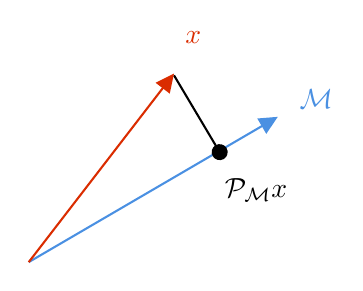
\begin{tikzpicture}[x=0.75pt,y=0.75pt,yscale=-1,xscale=1]
%uncomment if require: \path (0,300); %set diagram left start at 0, and has height of 300

%Straight Lines [id:da15401475064244685] 
\draw [color={rgb, 255:red, 74; green, 144; blue, 226 }  ,draw opacity=1 ]   (270,200) -- (387.41,131.51) ;
\draw [shift={(390,130)}, rotate = 149.74] [fill={rgb, 255:red, 74; green, 144; blue, 226 }  ,fill opacity=1 ][line width=0.08]  [draw opacity=0] (8.93,-4.29) -- (0,0) -- (8.93,4.29) -- cycle    ;
%Straight Lines [id:da5183541999539916] 
\draw    (340,110) -- (362,147) ;
\draw [shift={(362,147)}, rotate = 59.26] [color={rgb, 255:red, 0; green, 0; blue, 0 }  ][fill={rgb, 255:red, 0; green, 0; blue, 0 }  ][line width=0.75]      (0, 0) circle [x radius= 3.35, y radius= 3.35]   ;
%Straight Lines [id:da8459313489931962] 
\draw [color={rgb, 255:red, 218; green, 44; blue, 0 }  ,draw opacity=1 ]   (270,200) -- (338.17,111.52) ;
\draw [shift={(340,109.14)}, rotate = 127.61] [fill={rgb, 255:red, 218; green, 44; blue, 0 }  ,fill opacity=1 ][line width=0.08]  [draw opacity=0] (8.93,-4.29) -- (0,0) -- (8.93,4.29) -- cycle    ;

% Text Node
\draw (399,115.54) node [anchor=north west][inner sep=0.75pt]  [color={rgb, 255:red, 74; green, 144; blue, 226 }  ,opacity=1 ]  {$\mathcal{M}$};
% Text Node
\draw (344,87.54) node [anchor=north west][inner sep=0.75pt]  [color={rgb, 255:red, 218; green, 44; blue, 0 }  ,opacity=1 ]  {$\bm{x}$};
% Text Node
\draw (363,158.4) node [anchor=north west][inner sep=0.75pt]    {$\mathcal{P_{M}}\bm{x}$};


\end{tikzpicture}

    \caption{Projection in two-dimensional space}
    \label{fig:proj 2d}
\end{figure}

An equivalent statement is to say that $\mathcal{P}_\mathcal{M}$ is a square matrix. When this matrix is applied on $\bm{x}$, we get the projection onto the subspace $\mathcal{M}$. As projection theorem tells us, the projection of $\bm{x}$ onto $\mathcal{M}$ is the closest we can possibly get to $\bm{x}$ in the subspace. A bit of geometric intuition should tell you that this closest point forms an orthogonal error vector (shown in black). To make things clear, let's create a specific matrix $A$ whose column space spans $\mathcal{M}$. In this two-dimensional case, the column space will be a single vector. It's pretty clear that the closest point will be along this line. 

The closest point in our subspace will be a linear combination of the columns of $A$. We will denote this point as $A\hatx$. In this interpretation, $\hatx$ is the vector of coordinates that lie as close as possible to $\bm{x}$ in the subspace $\mathcal{M}$. The error in estimation will be the difference between the vector $\bm{x}$ and the closest point:
$$e=\bm{x}-A\hatx$$
Remember that the error vector must be perpendicular to the subspace $\mathcal{M}$. To ensure this, the error dotted with the vectors which comprise the span of $A$ must be zero. Stated another way, the error must be orthogonal to every basis vector of $\mathcal{M}$. Mathematically, this is like saying $A\cdot e=A^Te=0$. We can expand our expression for $e$ and the value of $\hatx$ can be attained:
\begin{gather}
A^T(\bm{x}-A\hatx)=0\\
A^T\bm{x} =A^TA\hatx\\
\hatx=(A^TA)^{-1}A^T\bm{x}
\end{gather}
This last equation should look familliar! The term on the left hand side is the pseudo-inverse that we found for least squares. We proved there that it produces an optimal estimate for a linear fit, and we see it again with projections. By multiplying with the $A$ matrix again, we get the projection of the vector:
$$A\hatx=\mathcal{P}_\mathcal{M}\bm{x}$$
This gives us the following for projections:
$$P_{\mathcal{M}}=A(A^TA)^{-1}A^T$$
This matrix has some interesting properties:
\begin{itemize}
    \item $\mathcal{P}$ is symmetric: $\mathcal{P}=\mathcal{P}^T$
    \item $\mathcal{P}^2=\mathcal{P}$
    \item $\mathcal{P}A=A$
\end{itemize}

The key point is this: \textbf{A projection is equivalent to least-squared minimization.} If you remember nothing else about projections, remember this! The two ideas are intimately related. Ultimately, using the language of projections will be more fruitful because Hilbert spaces can describe very abstract things. The underlying math is the same, but the way in which we frame things using Hilbert spaces will allow us to go much further.

\subsubsection{Higher Dimensions}
The Hilbert projection theorem is easily applicable to higher dimensions. We will go one dimension higher and see that the result still makes sense. We will consider the simple case of a Hilbert space  $\mathcal{H}\cong\mathbb{R}^3$ and the subspace $\mathcal{M}\cong\mathbb{R}^2$.\endnote{The $\cong$ symbol means \textit{isomorphic}. In this context we can treat it like an equality.} Our vector $\bm{x}$ can be represented with a point in $\mathbb{R}^3$.\endnote{The typical representation of a vector is an arrow from the origin to the tip (or any translation of this). To simplify the depiction, I'll only draw the endpoints.} Thus, the subspace $\mathcal{M}$ looks like a plane of points embedded in 3D space. 

\begin{figure}[ht]
    \centering



\tikzset{every picture/.style={line width=0.75pt}} %set default line width to 0.75pt        

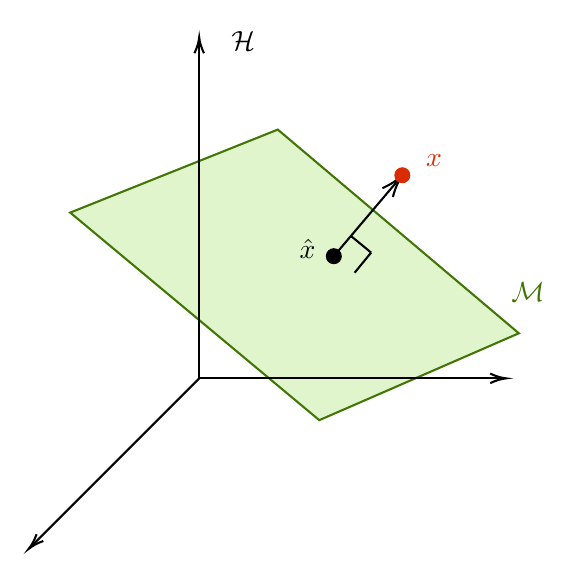
\begin{tikzpicture}[x=0.75pt,y=0.75pt,yscale=-1,xscale=1]
%uncomment if require: \path (0,300); %set diagram left start at 0, and has height of 300

%Shape: Polygon [id:ds7364872307144579] 
\draw  [color={rgb, 255:red, 65; green, 117; blue, 5 }  ,draw opacity=1 ][fill={rgb, 255:red, 126; green, 211; blue, 33 }  ,fill opacity=0.23 ] (250,90) -- (366.14,188.14) -- (270,230) -- (150,130) -- cycle ;
%Straight Lines [id:da18571977571671672] 
\draw    (277,151) -- (308.71,113.53) ;
\draw [shift={(310,112)}, rotate = 130.24] [color={rgb, 255:red, 0; green, 0; blue, 0 }  ][line width=0.75]    (10.93,-3.29) .. controls (6.95,-1.4) and (3.31,-0.3) .. (0,0) .. controls (3.31,0.3) and (6.95,1.4) .. (10.93,3.29)   ;
%Straight Lines [id:da875363957944581] 
\draw    (212.14,209.86) -- (212.14,47.57) ;
\draw [shift={(212.14,45.57)}, rotate = 90] [color={rgb, 255:red, 0; green, 0; blue, 0 }  ][line width=0.75]    (7.65,-2.3) .. controls (4.86,-0.97) and (2.31,-0.21) .. (0,0) .. controls (2.31,0.21) and (4.86,0.98) .. (7.65,2.3)   ;
%Straight Lines [id:da9276340728334019] 
\draw    (212.14,209.86) -- (358,209.86) ;
\draw [shift={(360,209.86)}, rotate = 180] [color={rgb, 255:red, 0; green, 0; blue, 0 }  ][line width=0.75]    (7.65,-2.3) .. controls (4.86,-0.97) and (2.31,-0.21) .. (0,0) .. controls (2.31,0.21) and (4.86,0.98) .. (7.65,2.3)   ;
%Straight Lines [id:da14439042039791194] 
\draw    (212.14,209.86) -- (131.41,290.59) ;
\draw [shift={(130,292)}, rotate = 315] [color={rgb, 255:red, 0; green, 0; blue, 0 }  ][line width=0.75]    (7.65,-2.3) .. controls (4.86,-0.97) and (2.31,-0.21) .. (0,0) .. controls (2.31,0.21) and (4.86,0.98) .. (7.65,2.3)   ;

%Straight Lines [id:da0867022872617943] 
\draw [color={rgb, 255:red, 218; green, 44; blue, 0 }  ,draw opacity=1 ]   (310,112) ;
\draw [shift={(310,112)}, rotate = 0] [color={rgb, 255:red, 218; green, 44; blue, 0 }  ,draw opacity=1 ][fill={rgb, 255:red, 218; green, 44; blue, 0 }  ,fill opacity=1 ][line width=0.75]      (0, 0) circle [x radius= 3.35, y radius= 3.35]   ;
%Straight Lines [id:da11541820586272067] 
\draw    (285.26,141.28) -- (294.98,149.26) ;
%Straight Lines [id:da1560785163363675] 
\draw    (294.98,149.26) -- (287,158.98) ;

%Straight Lines [id:da05441978974558226] 
\draw    (277,151) ;
\draw [shift={(277,151)}, rotate = 0] [color={rgb, 255:red, 0; green, 0; blue, 0 }  ][fill={rgb, 255:red, 0; green, 0; blue, 0 }  ][line width=0.75]      (0, 0) circle [x radius= 3.35, y radius= 3.35]   ;

% Text Node
\draw (361,162.4) node [anchor=north west][inner sep=0.75pt]  [color={rgb, 255:red, 65; green, 117; blue, 5 }  ,opacity=1 ]  {$\mathcal{M}$};
% Text Node
\draw (226.14,41.4) node [anchor=north west][inner sep=0.75pt]    {$\mathcal{H}$};
% Text Node
\draw (320,100.4) node [anchor=north west][inner sep=0.75pt]  [color={rgb, 255:red, 218; green, 44; blue, 0 }  ,opacity=1 ]  {$x$};
% Text Node
\draw (259,141.4) node [anchor=north west][inner sep=0.75pt]    {$\hat{x}$};


\end{tikzpicture}

   
    \caption{Geometric depiction of the Projection Theorem}
    \label{fig:proj thm geometric}
\end{figure}

This geometric depiction should make it obvious that the error vector, which we define as $\bm{\tilde{x}}=\bm{x}-\bm{\hat{x}}$, is orthogonal to the subspace $\mathcal{M}$. Any other point in the subspace will obviously have a larger distance from the point $\bm{x}$. It is only the unique point which has an orthogonal error vector which will produce the minimization of the error. This generalization will extend to higher dimensional spaces, though visualizing is beyond the capability of my drawing abilities.

Projection theorem gives us a powerful way to find an optimal solution to a problem in Hilbert space. If we may jump ahead and consider optimal estimation, we can see where this will become very useful: We have a true state which exists in $\mathcal{H}$ and our measurements and prior information which are in a subspace $\mathcal{M}$. The best we can possibly do is to find the minimum error vector between $\mathcal{H}$ and $\mathcal{M}$. The projection theorem gives us a way of finding a unique optimal solution to this problem.

With an intuition for projection theorem developed, we can move to a proof of the projection theorem.

\begin{proof}{Projection Theorem}
We'll start our proof by assuming our best estimate is a vector $\bm{\hat{x}}\in\mathcal{H}$. The error will be $\bm{x}-\bm{\hat{x}} \perp\mathcal{H}$. We compare to another vector in the space, $\bm{h}\in\mathcal{H}$. We start with:
$$\|\bm{x}-\bm{h}\|^2=\|\bm{x}-\bm{\hat{x}}+\bm{\hat{x}}-\bm{h}\|^2$$
We can expand this expression as follows:
$$\|\bm{x}-\bm{\hat{x}}\|^2+2\mathrm{Re}(\bm{x}-\bm{\hat{x}},\bm{\hat{x}}-\bm{h})+\|\bm{\hat{x}}-\bm{h}\|^2$$
Notice that the middle component will be zero, since the error is orthogonal to the components in the subspace. The subtraction of two components in the subspace is another element in the subspace. We therefore have:
$$\|\bm{x}-\bm{h}\|^2=\|\bm{x}-\bm{\hat{x}}\|^2+\|\bm{\hat{x}}-\bm{h}\|^2$$
From this, we can see that the magnitude of this error term must be less than or equal to this difference between $\|\bm{x}-\bm{h}\|^2$:
$$\|\bm{x}-\bm{h}\|^2=\|\bm{x}-\bm{\hat{x}}\|^2+\|\bm{\hat{x}}-\bm{h}\|^2\ge\|\bm{x}-\bm{\hat{x}}\|^2$$
We can simply this expression and take the square root to find that:
$$\|\bm{{x}}-\bm{h}\|\ge\|\bm{x}-\bm{\hat{x}}\|$$
We find that the value will result in the minimum error only when $\bm{h}$ and $\bm{\hat{x}}$ have zero distance: $\|\bm{\hat{x}}-\bm{h}\|=0$. This implies that our optimal estimate for the system is when $\bm{h}=\bm{\hat{x}}$. The result is that $\bm{\hat{x}}$ is the unique vector which minimizes the error in the system and establishes that $\bm{\hat{x}}=\mathcal{P}_\mathcal{H}\bm{x}$.
\end{proof}

\subsubsection{Estimation Error}
Projection theorem gives us a guarantee that we can find the closest possible estimate of a quantity, but some error will still exist. Quantifying this error is useful for determining the performance of any algorithm or method we may develop. Typically, we are concerned with the square of the error. We do this for the same reasons that we did in least squares estimation. Firstly, squaring the quantity means that positive and negative errors both still contribute to a total error. Additionally, quadratic terms have nicely behaved derivatives. As a result, we consider the squared error:
$$\|\bm{\tilde{x}}\|^2=\|\bm{x}-\bm{\hat{x}}\|^2$$
This is equivalent to writing the inner product of this vector with itself.
$$(\bm{x}-\bm{\hat{x}})^*(\bm{x}-\bm{\hat{x}})$$
We can expand this sum by multiplying each of the terms out:
$$\bm{x}^*\bm{x}-\bm{x}^*\bm{\hat{x}}-\bm{\hat{x}}^*\bm{x}+\bm{\hat{x}}^*\bm{\hat{x}}$$
We can expand the term $\bm{x}=\bm{\hat{x}}+\bm{\tilde{x}}$. Substituting this into our equation:
$$\bm{x}^*\bm{x}-(\bm{\hat{x}}+\bm{\tilde{x}})^*\bm{\hat{x}}-\bm{\hat{x}}^*(\bm{\hat{x}}+\bm{\tilde{x}})+\bm{\hat{x}}^*\bm{\hat{x}}$$
Since $\bm{\hat{x}}\perp\bm{\tilde{x}}$, those terms of the inner product will go to zero. We can then simplify this equation as:
$$\|\bm{x}\|^2-2\|\bm{\hat{x}}\|^2+\|\bm{\hat{x}}\|^2$$
We then find that the error in approximation will simply be:
$$\|\bm{x}-\bm{\hat{x}}\|^2=\|\bm{x}\|^2-\|\bm{\hat{x}}\|^2$$
Somewhat surprisingly, there is no coupling term between $\bm{x}$ and $\bm{\hat{x}}$ in the error vector. We can simply take the difference of their individual squares in order to describe the error in our estimation.

With that, we have established all the basic properties of Hilbert spaces that we need. We now have all the tools to discuss how we can relate the ideas of deterministic algorithms like the least squares to probabilistic ones like Bayes' theorem. To do so, we will introduce a specific Hilbert space for random variables.

\subsection{Hilbert Space of Random Variables}
Since random variables are random (of course), it doesn't make sense to talk about the `orthogonality' or `projection' of a random variable in the traditional sense. Because these variables can take on any number of values, we need to be really precise in describing how different random variables relate to each other. By describing things in terms of a Hilbert space, we can do that. Without losing any information, we can describe each random variable as some vector in an abstract Hilbert space. Only then does it make sense to talk about the orthogonality of two random variables. When we say that those vectors are orthogonal, we really mean that statistically, we would expect the two variables to have no relation to each other in the average of many trials. Because that's long and annoying to write out, we will instead develop the formalism of the Hilbert space of random variables.

We'll denote this Hilbert space as $\mathcal{H}=L^2(\Omega;\mathbb{R})$. This inner product space has the property that the variance of a variable is finite. Mathematically:
$$\mathcal{H}=\{\bm{X}:\bm{X} \text{ is r.v. and } \mathbb{E}\left[\bm{X}^2\right]<\infty\}$$
The inner product over this space is the expectation of two 
variables:
$$\bm{X}\cdot \bm{Y}=\mathbb{E}[\bm{XY}]$$
Wait a minute! I thought we chose to use the covariance as the inner product earlier. That's true, but we run into some issues when we try to create a Hilbert space that way. That's because the covariance of a constant is zero, and there should only be one zero function to define our inner product. If any constant could have a covariance of zero, we run into a few mathematical issues. We could remove constants from our space, but more often we just restrict ourselves to the study of mean-zero variables. In that case, we see that the covariance is exactly the same as the expectation between two variables:
$$\text{Cov}(\bm{X},\bm{Y})=\mathbb{E}[\bm{XY}]-\cancelto{0 \text{ for mean zero r.v.}}{\mu_X\mu_Y}$$
As we'll soon see, the Kalman filter only considers mean-zero variables. At the most basic mathematical level, this is one reason why. Using the expectation as the inner product is more well-founded than the covariance, and the two are only equal when we are using mean zero random variables.

Under the assumption of mean-zero variables (which we could denote $\mathcal{H}/\mathbb{R}$, we have the following properties:
\begin{enumerate}
    \item $\text{Cov}(\bm{XY})$ is the inner product. It can also be expressed as $\mathbb{E}(\bm{XY}^*)=R_{\bm{XY}}$
    \item $\sigma=\|\bm{X}\|$
    \item $\text{Var}(\bm{X})=\|\bm{X}\|^2$
    \item If $\bm{X}$ and $\bm{Y}$ are statistically uncorrelated, they are orthogonal in Hilbert space.
\end{enumerate}

This particular Hilbert space will be extremely useful for us. Now, we can use any of the tools we've developed for inner product spaces to understand random variables and their correlations.

\subsection{Projections for Random Variables}

By establishing a Hilbert space of random variables, we are able to understand the statistics of random variables. Here, we will explore that connection further by using the projection on a Hilbert space of random variables. We've already seen that the projection exactly matches what we get from least squares estimation. Now we will show that it will also reproduce the conditional probability for Gaussian random vectors. Thus, we will prove that the conditional expectation, the projection, and least squares are all identical methodologies.

Suppose we have two Gaussian random vectors, $\bm{X}$ and $\bm{Y}$. We want to understand the conditional probability of the two variables, $\mathbb{E}(\bm{X}|\bm{Y})$. The random vector $\bm{X}$ has the interpretation of a state that is not fully observed or hidden. The random vector $\bm{Y}$ are system measurements.

We remember from Bayesian statistics that the optimal estimate $\bm{\hat{X}}$ is the same as this conditional probability. For Gaussian variables, we showed that this optimal estimate was some linear update. Since we are concerned with zero-mean random vectors here, we can express the optimal estimate quite simply as some constant matrix $\bm{K}$ multiplied by the measurement. If we had non-zero mean random vectors, there would we an additional term for the mean of the variable:
\begin{equation}
\hat{\bm{X}} = \bm{K}\bm{Y}
\end{equation}
By the Projection Theorem in Hilbert spaces, the estimation error vector $\tilde{\bm{X}} = \bm{X} - \hat{\bm{X}}$ must be orthogonal to every vector in the measurement subspace. 

Because the subspace is generated by $\bm{Y}$, this orthogonality condition dictates that the inner product between the estimation error and the measurement vector must equal zero:
\begin{equation}
( \bm{X} - \bm{K}\bm{Y}, \bm{Y} ) = \mathbb{E}\left[ (\bm{X} - \bm{K}\bm{Y})\bm{Y}^* \right] = \bm{0}
\end{equation}
Using the linearity of the expectation operator, we can expand this directly:
\begin{equation}
\mathbb{E}[\bm{X}\bm{Y}^*] - \bm{K}\mathbb{E}[\bm{Y}\bm{Y}^*] = \bm{0}
\end{equation}
Notice that these expectations are the exact definition of the cross-correlation matrix ${R}_{\bm{X}\bm{Y}}$ and the measurement auto-correlation matrix ${R}_{\bm{Y}}$ for our zero-mean vectors. Substituting these terms into our equation yields:
\begin{equation}
{R}_{\bm{X}\bm{Y}} - \bm{K}{R}_{\bm{Y}} = \bm{0}
\end{equation}
Isolating the matrix $\bm{K}$ by multiplying both sides by the inverse of the measurement auto-correlation matrix, we find:
\begin{equation}
\bm{K} = {R}_{\bm{X}\bm{Y}} {R}_{\bm{Y}}^{-1}
\end{equation}
Substituting this optimal gain matrix back into our original linear estimator expression, we arrive at the final geometric state estimate:
\begin{equation}
\hat{\bm{X}} = {R}_{\bm{X}\bm{Y}} {R}_{\bm{Y}}^{-1} \bm{Y}
\end{equation}
From here on out, we will maintain the bold face to signify that our quantities like $\bm{x}$ are vectors, but will revert back to lower case letters which are more typical in controls applications. Therefore, we have the following that are all equivalent:
$$\bm{\hat{x}}=\mathcal{P}_\mathcal{M}\bm{x}=R_{\bm{xy}}R_{\bm{y}}^{-1}\bm{y}=\mathbb{E}(\bm{x}|\bm{y})$$
This is quite the accomplishment. We now have a simple way to turn relate the probabilistic and deterministic views together, and can compute an optimal state estimate.

\subsubsection{Projection Error}
Previously, we were able to compute the error in estimation in general for Hilbert spaces. Let's apply that approach specifically the the Hilbert space of random variables. We'll remember that the error in estimation was given by:
$$\|\bm{x}-\bm{\hat{x}}\|^2=\|\bm{x}\|^2-\|\bm{\hat{x}}\|^2$$
In the Hilbert space of random variables, the equivalent representation uses the zero-mean covariance:
$$\mathbb{E}(\bm{x\bm{x}^*})-\mathbb{E}(\bm{\hat{x}}\bm{\hat{x}}^*)$$
We recognize that the first matrix is simply the autocorrelation function for $\bm{x}$. The second term requires that we substitute in our expression for $\bm{\hat{x}}$:
$$R_{\bm{x}}-\mathbb{E}\left[\left(R_{\bm{xy}}R_{\bm{y}}^{-1}\bm{y}\right)\left(R_{\bm{xy}}R_{\bm{y}}^{-1}\bm{y}\right)^*\right]$$
Since the auto and cross-correlation matrices are constant matrices, we can pull them outside the expectation:
$$R_{\bm{x}}-\left(R_{\bm{xy}}R_{\bm{y}}^{-1}\right)\mathbb{E}\left[\bm{y}\bm{y}^*\right]\left({R_{\bm{y}}^{-1}}^*R_{\bm{xy}}^*\right)$$
Notice that the autocorrelation function (and it's inverse) are symmetric Hermitian matrices. The cross-correlation matrices are conjugate symmetric. Using the fact that $\mathbb{E}\left[\bm{y}\bm{y}^*\right]=R_{\bm{y}}$, we get the following:
$$R_{\bm{x}}-R_{\bm{xy}}\cancel{R_{\bm{y}}^{-1}R_{\bm{y}}}{R_{\bm{y}}^{-1}}R_{\bm{yx}}=R_{\bm{x}}-R_{\bm{xy}}{R_{\bm{y}}^{-1}}R_{\bm{yx}}$$
As a result, we find that the squared error in estimation will be:
$$\|\bm{\tilde{x}}\|^2=R_{\bm{x}}-R_{\bm{xy}}{R_{\bm{y}}^{-1}}R_{\bm{yx}}$$
As with our state estimate, we find that the error will be a linear function of the state. In fact, it only depends on the correlation matrices for the system. Our final step will be to express the state estimate and the error estimate in terms of an orthogonal set of basis vectors. To do that, we will invoke the Gram-Schmidt process for creating an orthogonal basis.

\subsection{Gram-Schmidt}

In the previous section, we established that the optimal estimate of a hidden state is achieved by projecting it orthogonally onto a subspace spanned by our measurements. However, when dealing with a sequential stream of data—such as a sequence of sensor measurements $\bm{y}_1, \bm{y}_2, \dots, \bm{y}_k$—the standard projection equations quickly become computationally intractable. Because sensor data is sequentially correlated, the measurement history forms a non-orthogonal basis for the subspace. To invert the resulting multi-variable correlation matrices in real time, we need a way to decorrelate the data stream as it arrives.

This is exactly where the classical Gram-Schmidt orthogonalization process becomes our primary tool. Gram-Schmidt orthogonalization allows us to take a sequence of non-orthogonal measurement vectors and systematically construct an equivalent, mutually orthogonal basis. In the context of stochastic filtering, these orthogonal basis vectors are called \textit{innovations}.

Let us denote the subspace spanned by all measurements up to time step $k-1$ as a Hilbert space $\mathcal{Y}_{k-1}$:
\begin{equation}
\mathcal{Y}_{k} = \text{span}\{\bm{y}_1, \bm{y}_2, \dots, \bm{y}_{k-1}\}
\end{equation}
When a new measurement vector $\bm{y}_k$ arrives at time step $k$, it is generally not orthogonal to the existing space $\mathcal{Y}_{k-1}$. Following the standard Gram-Schmidt methodology, we can isolate the orthogonal component of this new measurement by subtracting its projection onto the prior subspace. We will call this new orthogonal component $\varphi_k$ to differentiate it from the standard non-orthogonal measurements:
\begin{equation}
\varphi_k = \bm{y}_k - \mathcal{P}_{\mathcal{Y}_{k-1}}(\bm{y}_k)
\end{equation}
Because we established that an orthogonal projection onto a Hilbert subspace of random variables is identical to the conditional expectation, we can replace the projection operator with our probabilistic notation:
\begin{equation}
\varphi_k = \bm{y}_k - \mathbb{E}[\bm{y}_k \mid \mathcal{Y}_{k-1}]
\end{equation}
The vector $\varphi_k$ is the \textit{innovation} (or residual) at time step $k$. It represents the entirely new information brought in by the sensor that could not have been anticipated from past data. By applying this process recursively, we transform our correlated measurement sequence into an orthogonal innovation sequence $\{\varphi_1, \varphi_2, \dots, \varphi_k\}$, which satisfies:
\begin{equation}
( \varphi_i, \varphi_j )= \mathbb{E}[\varphi_i \varphi_j^T] = \bm{0} \quad \text{for } i \neq j
\end{equation}
This orthogonal basis fundamentally changes how we compute the state update. Instead of projecting our hidden state $\bm{x}_k$ onto the unwieldy, coupled history of raw measurements, we can project it onto the clean, decoupled innovations. Because the innovations are mutually orthogonal, the total projection splits into an independent sum of projections across each individual time step:
$$\bm{\hat{x}}_n=\sum_{k=0}^{n-1}R_{\bm{x}_n \varphi_k} R_{\varphi_{k}}^{-1}\varphi_k$$
Notice that nothing fundamental has changed. Our state estimate is still linear and only depends on the current state and the measurements (represented through $\varphi_k$). Through Gram-Schmidt orthogonalization, we have naturally derived the exact methodology that we will use in Kalman filtering. The expression demonstrates that the current estimate is simply the prior estimate corrected by a linear weighting of the innovation vector.

With that, we have developed all the background we need in order to develop the Kalman filter in the next chapter. Before we do that, we will investigate one other use case of Hilbert spaces in control theory.

\section{Controllability \& Observability Gramian}
Let's remember our discussion of controllability and observability from the last chapter. There, we were able to develop tools to understand when a system was controllable or observable at all. 
In designing controllers and observers, it is often useful to know controllable or observable our system is. While the standard controllability and observability conditions will tell us if the system is controllable or observable at all, the Gramian\footnote{Named after J{\o}rgen Gram, Danish Mathematician} will tell us which modes of the system are most controllable / observable. The test will only work with systems for which $A$ is Hurwitz. We will first focus on the controllability condition. We can easily convert to the observability condition using the already established duality.

The derivation of the controllability Gramian will require some of the theory of Hilbert spaces and least squares estimation, which will make it a perfect use case for the theory we have developed throughout this chapter. This will give us some time to tackle an example of Hilbert spaces and optimization problems before we go to the full Kalman filter.

\subsection{Derivation of the Controllability Gramian}
The basic idea is to start at some point in our space and consider a bounded control input $u$. In directions that are easy to travel in, we can go further. In directions that are hard to travel in, we cannot go as far. Directions which are easily traversable have high controllability. In general, the combination of all possible directions will form an ellipsoid in some vector space. The best parameterization of the ellipsoid for us will be related to the eigenvalues of the system. We can visualize the two dimensional case easily:
\begin{figure}
    \centering


\tikzset{every picture/.style={line width=0.75pt}} %set default line width to 0.75pt        

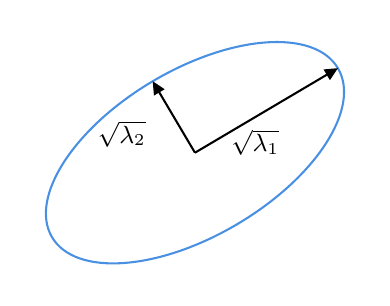
\begin{tikzpicture}[x=0.75pt,y=0.75pt,yscale=-1,xscale=1]
%uncomment if require: \path (0,300); %set diagram left start at 0, and has height of 300

%Shape: Ellipse [id:dp8968156888700339] 
\draw  [color={rgb, 255:red, 74; green, 144; blue, 226 }  ,draw opacity=1 ] (231.14,170.72) .. controls (219.9,151.71) and (241.61,118.06) .. (279.64,95.57) .. controls (317.67,73.08) and (357.61,70.26) .. (368.86,89.28) .. controls (380.1,108.29) and (358.39,141.94) .. (320.36,164.43) .. controls (282.33,186.92) and (242.39,189.74) .. (231.14,170.72) -- cycle ;
%Straight Lines [id:da5296520615305047] 
\draw    (300,130) -- (281.17,98.15) ;
\draw [shift={(279.64,95.57)}, rotate = 59.4] [fill={rgb, 255:red, 0; green, 0; blue, 0 }  ][line width=0.08]  [draw opacity=0] (6.25,-3) -- (0,0) -- (6.25,3) -- cycle    ;
%Straight Lines [id:da9869271122040867] 
\draw    (300,130) -- (366.28,90.8) ;
\draw [shift={(368.86,89.28)}, rotate = 149.4] [fill={rgb, 255:red, 0; green, 0; blue, 0 }  ][line width=0.08]  [draw opacity=0] (6.25,-3) -- (0,0) -- (6.25,3) -- cycle    ;

% Text Node
\draw (316,117.31) node [anchor=north west][inner sep=0.75pt]  [font=\small]  {$\sqrt{\lambda _{1}}$};
% Text Node
\draw (251.75,113.24) node [anchor=north west][inner sep=0.75pt]  [font=\small]  {$\sqrt{\lambda _{2}}$};


\end{tikzpicture}

    \caption{Eigenvalue decomposition of ellipsoid}
    \label{fig:ellipsoid}
\end{figure}
Mathematically, this system will be represented by a quadratic matrix inequality. This will look like:
$$E=\{x\in\mathbb{R}^n;x^*Q^{-1}x\le1\}$$

Here, a star is used for the conjugate transpose of a matrix and  $\lambda$ are the eigenvalues of the $Q$ matrix. The $Q$ matrix is positive and symmetric. We can see how such a parameterization would look to a diagonal matrix with the eigenvalues and the eigenvectors pointing in the directions of the semi-axes of the ellipse. Our basic goal is to figure out what such an ellipsoid would look like for a control system.

\begin{exercise}
Expand the matrix equation $x^*Q^{-1}x\le1$ in the case of a 2 dimensions and prove it is the same as the standard equation for an ellipse. Start simply with a diagonal matrix $Q$, but show how a general rotated ellipse is also possible.
\end{exercise}

We want to come up with an alternate representation of this ellipsoid. I'll cover our basic intent for the proof now. We will start by creating a new representation and showing that it is a subset of the representation we just made. If we call our first representation $E_1$ and the new representation $E_2$, we want to show:
$$E_2\subset E_1$$
We'll then go the other way, and show that $E_1\subset E_2$. Of course, if both sets are subsets of each other, they are the same set. That's the basic premise. To make things precise, here are the definitions for $E_1$ and $E_2$ that we will be using:
$$E_1=\{x\in\mathbb{R}^n;x^*Q^{-1}x\le1\}$$
$$E_2=\{Mu;u\in\mathcal{U},\|u\|^2\le1\}$$

\subsubsection{Showing $E_2\subset E_1$}

Let's think about a Hilbert space $\mathcal{U}$ which our control vector resides in such that $u\in\mathcal{U}$. We want to limit this control input to have a 2-norm with length $1$ so that we trace out such an ellipsoid for our system. By ensuring the length cannot exceed 1, we can check which directions are the hardest to move in given a $u$ of only 1. Physically, this is equivalent to enforcing a constraint on the energy of the system. It is in fact related to the inner product definition we had in classical control
$$\int u(t)u^*(t)dt\le1$$
We'll still want to incorporate our matrix $Q$, but we'll now consider a matrix $M$ such that $Q=MM^*$. The matrix $M$ is a mapping which takes us from the Hilbert space into the real space $\mathbb{R}^n$:
$$M:\mathcal{U}\rightarrow\mathbb{R}^n$$
Because $M$ is such a mapping, there will be some $u$ for which the mapping $M$ will give us the state $x$ via $x=Mu$. A direct substitution of these variables into $E_1$ gives us the following:
$$E=\{Mu\in\mathbb{R}^n;u^*M^*Q^{-1}Mu\le1\}$$
Let's investigate the second part of this condition. We have the equality
$$x^*Q^{-1}x=u^*M^*Q^{-1}Mu$$
We notice that this can be represented as an inner product:
$$x^*Q^{-1}x=(u,M^*(MM^*)^{-1}Mu)$$
The term $M^*(MM^*)^{-1}M$ is an underdetermined pseudoinverse multiplied by $M$. This is a projection operation. It projects the Hilbert space $\mathcal{U}$ onto the range of $M^*$. Thus we have:
$$x^*Q^{-1}x=(u,Pu)$$
Remember that a projection has the property that $P=P^2$ and $P=P^*$. Therefore, the inner product is equivalently:
$$x^*Q^{-1}x=(Pu,Pu)$$
A simple argument shows that the norm of $P$ must be less than or equal to 1 for the above properties to hold. We also assumed that the input $u$ was less than or equal to one. We now have a bounding condition that:
$$x^*Q^{-1}x=(Pu,Pu)\le1$$
This argument shows directly that $E_2\subset E_1$, since it must be bounded less than or equal to 1 just as $E_1$ is.

\subsubsection{Showing $E_1\subset E_2$}
With the idea established that $E_2$ is a subset of $E_1$, we will proceed to show that the opposite must be true as well. We'll start by establishing our control as:
$$u=M^*(MM^*)^{-1}x$$
You may check the dimensions of the matrix to verify that the mapping will indeed keep $u$ in the Hilbert space $\mathcal{U}$. We suppose here that $x\in E_1$ such that $x^*Q^{-1}x\le1$. Now, we multiply both sides of our equation on the left by $M$:
$$Mu=MM^*(MM^*)^{-1}x$$
It should be obvious that the $MM^*$ terms cancel to the identity and we find the equivalence:
$$Mu=x$$
So we have shown the first part is true under this choice of $u$. We now should show that the 2-norm of $u$ is bounded to less than 1. We can do so by directly computing the inner product:
$$(u,u)=(M^*(MM^*)^{-1}x,M^*(MM^*)^{-1}x)$$
We can then move all the terms in $M$ to the right hand side of the inner product using the adjoint property
$$(u,u)=(x,(MM^*)^{-1}MM^*(MM^*)^{-1}x)$$
From which we see that one pair $(MM^*)^{-1}MM^*$ will cancel and we are left with:
$$(u,u)=x^*Q^{-1}x\le1$$
Therefore we have shown that indeed $E_1\subset E_2$ and the two sets are indeed identical. With this knowledge, we can represent our control problem in a very similar way.

\subsubsection{Relating the Ellipsoid to Control Systems}
We are now ready to relate this ellipsoid to a control system. Let's imagine that our ellipse of controllable points is $E_c$. We can represent the ellipse with a matrix $X_c$ such that $\xi^*X_c^{-1}\xi\le1$. As we have seen, an equivalent representation exists with the control vector. We simply decompose $X_c=\Psi_c\Psi_c^*$.Such a factorization can easily be computed with the Cholesky factorization since $X_c$ is a positive definite symmetric matrix. Use \texttt{chol} in Matlab to do such a decomposition. Then, the ellipse is equivalently given by:
$$E_c=\{\Psi_c u;u\in L^2(-\infty,0],\|u\|^2\le1\}$$
Here we take our Hilbert space to be the Lebesgue space over the interval from $-\infty$ to $0$. Remember that the Lebesgue space is a very standard space for physics and controls applications. The matrix $\Psi_c$ is a transform from this Hilbert space into $\mathbb{R}^n$ as before. It is natural for us to define this transformation in terms of the inner product of the state evolution and the control in this Lebesgue space, which is:
$$\Psi_cu=\int_{-\infty}^0e^{-A\tau}Bu(\tau)d\tau$$
We find that the operator itself is just:
$$\Psi_c=\int_{-\infty}^0e^{-A\tau}Bd\tau$$
To find the function $X_c$, we simply need to multiply $\Psi_c$ with its conjugate. We find that this is:
$$X_c=\Psi_c\Psi_c^*=\int_{-\infty}^0e^{-A\tau}BB^*e^{-A^*\tau}d\tau$$
We can flip the integral to reverse the sign on the exponential functions. This will yield our final expression:
\begin{gather}
\color{boxBlue}\boxed{\color{black}X_c=\Psi_c\Psi_c^*=\int_0^\infty e^{A\tau}BB^*e^{A^*\tau}d\tau}\\
\color{boxBlue}\text{Controllability Gramian}
\end{gather}
By computing this expression we may find the matrix $X_c$ which tells us the directions / modes in which our system is easily controllable. Large eigenvalues of the matrix correspond to easily controllable directions, and small eigenvalues to directions which are not easily controlled. The eigenvectors correspond to the semi axes of the ellipse.

Often, computing this infinite time integral is somewhat difficult. For systems that are Hurwitz (open loop stable), we can calculate the value of $X_c$ in a simpler way. We consider the so-called \textit{Lyapunov} equation:
$$AX_c+X_cA^*=-BB^*$$
We can directly plug in our integral equation for $X_c$ to see that this result is true. We have:
$$\int_0^\infty Ae^{A\tau}BB^*e^{A^*\tau}d\tau+\int_0^\infty e^{A\tau}BB^*e^{A^*\tau}A^*d\tau =BB^*$$
Let's combine these integrals into a single one:
$$\int_0^\infty Ae^{A\tau}BB^*e^{A^*\tau}+e^{A\tau}BB^*e^{A^*\tau}A^*d\tau =BB^*$$
Notice that the integrand is the same as:
$$\frac{d}{d\tau}\left(e^{A\tau }BB^*e^{A^*\tau}\right)$$
We can substitute this in and use the fundamental theorem of calculus:
$$\lim_{\tau\rightarrow\infty} \left(e^{A\tau }BB^*e^{A^*\tau}\right)-e^{A0 }BB^*e^{A^*0}=BB^*$$
Since $A$ is Hurwitz, the limit at infinity will reduce to zero. At zero, we have $e^0=I$ and our expression reduced to the equality:
$$BB^*=BB^*$$
The result is that we can solve the Lyapunov equation $AX_c+X_cA^*=-BB^*$ instead of the integral in order to find $X_c$. This problem is often much more tractable. We can solve such Lyapunov equations in Matlab using the \texttt{lyap} command. In this situation, we can also use the \texttt{gram} command to find the $X_c$ matrix. Both will give the same result.
\begin{matlabscript}{}
A = [0 1;-1 -1];
B = [0;1];
C = [0 1];
D = 0;

% lyapunov approach:
Xc1 = lyap(A,B*B')

sys = ss(A,B,C,D);

% matlab built-in
Xc2 = gram(sys,"c")
\end{matlabscript}
Both approaches will yield the same resulting $X_c$ matrix. The \texttt{gram} function is often more useful for this specific case because we may also return the Cholesky factorization of $X_c$ (giving the $\Psi_c$ matrices) by using the specification \texttt{cf} instead of \texttt{c}. We may also replace \texttt{c} with \texttt{o} for the observability Gramian, which is the next topic of discussion.

\subsection{Observability Gramian}

The observability Gramian is very similar to the controllability Gramian, but we perform the suitable translation into the dual space. To get the final result, it is as simple as replacing the appropriate matrices. Note that when we use the complex conjugate `$*$', these identities are:
\begin{gather}
A_\text{ctrb}=A_\text{obsv}^*\\
B_\text{ctrb}=C_\text{obsv}^*\\
C_\text{ctrb}=B_\text{obsv}^*\\
D_\text{ctrb}=D_\text{obsv}^*\\
\end{gather}
The resulting observability gramian is:
\begin{gather}
\color{boxBlue}\boxed{\color{black}X_o=\int_0^\infty e^{A^*\tau}C^*Ce^{A\tau}d\tau}\\
\color{boxBlue}\text{Observability Gramian}
\end{gather}
The interpretation is much the same as the controllability Gramian. Large eigenvalues correspond the easily observed states of the system. Just as the controllability Gramian uses the geometry of Hilbert space projections to bound the state reachability given a limited control input, the observability Gramian bounds our estimation certainty given noisy measurements. This exact framework of projections and quadratic forms will serve as the foundation for deriving the optimal estimator: the Kalman filter. 

\newpage
\printendnotes

\chapter{Kalman Filtering}\label{chap:kalman}
\begin{chapquote}{Kyoto Prize committee}
The creator of modern control and system theory, Kalman theory, which was established in the early 1960s, brought a fundamental reformation to control engineering and since then laid the foundation for the rapid progress of modern control theory. 
\end{chapquote}

It is not an exaggeration to say that the development of Kalman filtering facilitated many of advances which have led to modern control theory. The prominent use of state space models can, in large part, be attributed to the development of Kalman Filtering. As we will see, the natural language to express the Kalman filter is with state space models.

We've spent some time in the previous chapter developing the background which will be necessary to derive the Kalman Filter. Before we get into the derivation of the filter, it is a good idea to make sure we have an understanding of why we even need the Kalman filter. If we have a system output that we measure directly with a sensor, why do we need to estimate it?

There are two main reasons to apply estimation. First, no true sensor is perfect. There are always errors and uncertainties associated with any sensor. When we want to take a derivative of a signal, things get much worse. True signals have noise and taking derivatives makes things very noisy or unusable. Optimal estimation provides us a way to reduce uncertainties in the most optimal way and get the best possible estimates of the true state. The second reason is that we can use estimation to gain an understanding of states that we cannot directly observe. This is very useful for us in many applications! For example, if we are flying our rocket, there is no instrument that we can use to measure our drag coefficient, $C_D$. However, we can apply optimal estimation to get a very good estimate of the $C_D$ nonetheless.

The most common way to perform optimal estimation is with the Kalman Filter. In the case of gaussian random vectors, the Kalman filter is the optimal filter for a linear system. As with control systems, understanding the theory of the linear systems will be useful even as we extend our scope to non-linear systems. As such, this chapter is devoted to understanding the Kalman filter and applying it to linear systems. After that, we'll extend it's use to non-linear systems and expand beyond the Kalman filter.

If you're not already convinced of the Kalman Filter's greatness, I will motivate the discussion by looking at a few examples. Say we want to measure the temperature of a rocket engine exhaust. We have a physical constraint on the system that any thermometer will melt under the heat of a rocket engine. What can we do then?

We can put a thermometer on the outside of the engine and measure the temperature there. If we know the metal the engine is made of and some properties of our cooling system, we can construct a pretty good model of what the heat transfer across the engine will look like. In other words, we build a model that tells us what we should expect. You know by now that our model corresponds to our $A$ matrix.

Of course, we can also correlate this temperature with some other sensors, say a barometer, to measure aspects of temperature that are tied to the pressure reading. This type of analysis is commonly referred to as \textit{sensor fusion} and is another useful property of the Kalman Filter.

This example touches on some key aspects of the Kalman Filter. Firstly, we need a good model of our system for a Kalman Filter to work. This is because the Kalman Filter effectively acts as a real time numerical integrator! We have to update our model in real time to help us model the system behavior. The other important aspect of the Kalman Filter is that we need measurements, and more importantly, we need to understand how those measurements are related to each other. This need to understand measurements and random noise is the role of statistics in the Kalman filter.

\subsubsection{Kalman Filtering Outline}
This chapter and the next chapter are long enough that they facilitate their own outline. We'll start things with the theory for linear systems, which are all mathematically well founded and rigorous. This chapter will focus on that domain, the linear Kalman filter. Even considering only linear systems, we still have quite a few varieties to explore. There's the discrete time case, the continuous time case, and Kalman filtering with control.

In the next chapter, we'll move on from linear systems to explore how we can do filtering for non-linear systems. We'll use some extensions of the Kalman filter to help us do that. Some popular extensions include the extended Kalman filter and the unscented Kalman filter. There are also some filter implementations which are specific to aerospace applications, such as the multiplicative filter. I will briefly touch on all of these types of filters in the following chapter. I have chosen to devote this time to the Kalman filter because almost all practical systems require such a filter. It is very rare that your sensors are good enough for direct use.

\section{What is Filtering?}
Before we dive deeply into the Kalman filter itself, we should understand what filtering even means in the time domain. Filtering is the estimation of a data point at the current time. A more technical definition might be:
\begin{definition}[Filtering]
    Filtering is the recursive estimation of parameters of interest, $\bm{x}$ based on measurements $\bm{y}$.
\end{definition}

Filtering, then, can be thought of as real-time estimation of parameters, using all of the current knowledge of the system to make a best estimate of what $\bm{x}$ is.

Notably, there are two other types of analysis that we can do: smoothing and prediction. A smoothing algorithm uses data up to the current time to make a prediction of $\bm{x}$ at an earlier time. A predictor does the opposite, and attempts to make a best guess of $\bm{x}$ at a future time given the current measurement data. We can represent these differences graphically, as shown in \autoref{fig:filter smooth}.

\begin{figure}[ht]
    \centering

\tikzset{every picture/.style={line width=0.75pt}} %set default line width to 0.75pt        

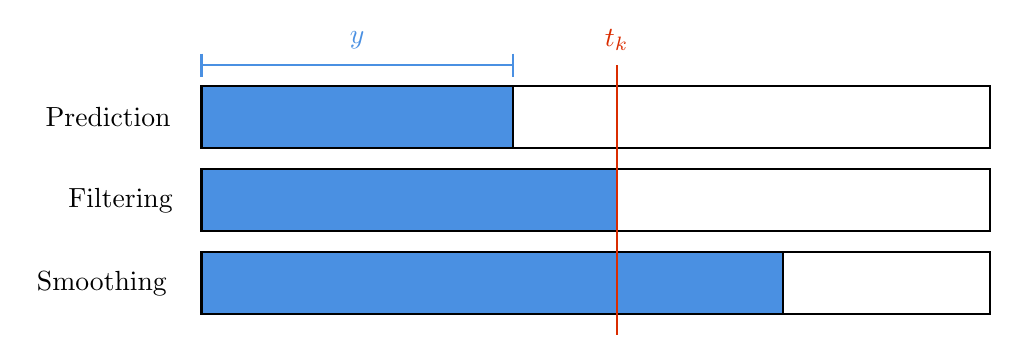
\begin{tikzpicture}[x=0.75pt,y=0.75pt,yscale=-1,xscale=1]
%uncomment if require: \path (0,300); %set diagram left start at 0, and has height of 300

%Shape: Rectangle [id:dp4331626883038564] 
\draw   (140,120) -- (520,120) -- (520,150) -- (140,150) -- cycle ;
%Shape: Rectangle [id:dp837454316770156] 
\draw  [fill={rgb, 255:red, 74; green, 144; blue, 226 }  ,fill opacity=1 ] (140,120) -- (290,120) -- (290,150) -- (140,150) -- cycle ;
%Shape: Rectangle [id:dp8012731044569247] 
\draw   (140,160) -- (520,160) -- (520,190) -- (140,190) -- cycle ;
%Shape: Rectangle [id:dp9224085547394635] 
\draw  [fill={rgb, 255:red, 74; green, 144; blue, 226 }  ,fill opacity=1 ] (140,160) -- (340,160) -- (340,190) -- (140,190) -- cycle ;
%Shape: Rectangle [id:dp9267874961996666] 
\draw   (140,200) -- (520,200) -- (520,230) -- (140,230) -- cycle ;
%Shape: Rectangle [id:dp3599207094201875] 
\draw  [fill={rgb, 255:red, 74; green, 144; blue, 226 }  ,fill opacity=1 ] (140,200) -- (420,200) -- (420,230) -- (140,230) -- cycle ;
%Straight Lines [id:da29650593501848965] 
\draw [color={rgb, 255:red, 218; green, 44; blue, 0 }  ,draw opacity=1 ]   (340,110) -- (340,240) ;
%Straight Lines [id:da21956457908837723] 
\draw [color={rgb, 255:red, 74; green, 144; blue, 226 }  ,draw opacity=1 ]   (140,110) -- (290,110) ;
\draw [shift={(290,110)}, rotate = 180] [color={rgb, 255:red, 74; green, 144; blue, 226 }  ,draw opacity=1 ][line width=0.75]    (0,5.59) -- (0,-5.59)   ;
\draw [shift={(140,110)}, rotate = 180] [color={rgb, 255:red, 74; green, 144; blue, 226 }  ,draw opacity=1 ][line width=0.75]    (0,5.59) -- (0,-5.59)   ;

% Text Node
\draw (340,104.6) node [anchor=south] [inner sep=0.75pt]  [color={rgb, 255:red, 218; green, 44; blue, 0 }  ,opacity=1 ]  {$t_{k}$};
% Text Node
\draw (95,135) node   [align=left] {Prediction};
% Text Node
\draw (101,175) node   [align=left] {Filtering};
% Text Node
\draw (92,215) node   [align=left] {Smoothing};
% Text Node
\draw (215,103.6) node [anchor=south] [inner sep=0.75pt]  [color={rgb, 255:red, 74; green, 144; blue, 226 }  ,opacity=1 ]  {$y$};


\end{tikzpicture}

    
    \caption{Prediction, Smoothing, and Filtering}
    \label{fig:filter smooth}
\end{figure}

A lot of the times, we model systems in discrete time and not in continuous time because that's what modern electronic systems are best suited to handle. In that case, `filtering' is a bit of a misnomer. Most of our algorithms will take data from 1 step ago and predict it forward, and then filter the estimate from the current step. Either way, we're normally only doing one time step into the past and calling it filtering is not far from the truth. That's why we often write the Kalman filter as a two-step algorithm: a prediction step and filtering/smoothing step. Beyond one step ahead or beyond, smoothing and prediction will not be touched on in this book. For the most part, these algorithms are fairly simple extensions of the Kalman Filter. However, they are not as useful as the simple filtering algorithm for real time applications.

While we are here, we'll go ahead and introduce some notation for the prediction and filtering. These are:
\begin{align}
\bm{x}(n|n-1)&\rightarrow\text{predicting $n$ from $n-1$ data} \\
\bm{x}(n|n)&\rightarrow\text{smoothing $n$  from $n$ data}
\end{align}
Notice that this is the same notation as a conditional expectation. That's because it \textit{is} a conditional expectation. Our study of Bayesian statistics and Hilbert space will soon become useful!

\section{Building The Kalman Filter}
Our previous discussions on statistics and least squares estimation has finally led us to discuss the Kalman filter. The Kalman filter is a filter which provides the best possible estimate for a linear system. We'll start our discussion by building the appropriate state space model for estimation problems. Then, we will be able to apply our knowledge from the previous chapter in order to do a mathematical derivation of the filter. Throughout this mathematical derivation, we will include some intuitions for the filter. Both the intuition and mathematical rigor will be needed to fully understand the Kalman Filter. 

\subsection{Criteria of Optimality}

Our criteria of optimality is the goal we hope to achieve with our estimator. The best possible estimate of a state in a system is \textit{unbiased}, \textit{minimum variance}, and \textit{consistent}. An unbiased estimator has the property that the expected value from the sensor is the same as the true value. This effectively means that the sensor is accurate, although it may not provide particularly precise measurements. The second quality is that of minimum variance. This is effectively the criteria of optimality, in that no other estimator can provide a lower variance than the minimum variance system. Finally, a consistent estimator converges to the true value of the state. A Kalman Filter has all of these properties.

It is important to note that there is a subtle distinction between a consistent and an unbiased estimator. A consistent estimator may converge at $t\rightarrow\infty$ to the true value of $\bm{x}$, but at any time prior its estimate does not agree with the true value. This can be seen quite evidently in \autoref{fig:consist est}.

\begin{figure}[ht]
    \centering
    \includesvg[width=0.75\linewidth]{Images/Consistency_of_estimator}
    \caption{A consistent but biased estimator \cite{stpasha_consistent_nodate}}
    \label{fig:consist est}
\end{figure}
\todo{redo this figure}

An estimator can converge to the true value while having estimates of the state that are not centered around the true mean! This is not what we want for Kalman filtering. Therefore, we require not only a consistent but also an unbiased estimator. Our method of Bayesian statistics has already shown that we can produce a MMSE error. Through the derivation of the filter, we will be able to show that there is no bias in the filter and that it is also consistent.

Having defined the notion of optimality and the constraints of the system, we can proceed with the derivation of the Kalman filter. With these goals in mind, let's set up the state space for our Kalman filter. We're going to do everything in discrete time, because it's much easier than continuous time. I think the reader will appreciate the easier derivation.

\subsection{The State Space}

Our state space will look similar to the standard discrete time model, but we will replace the control in the system by noise. We will eventually add control back into the system. From the criteria that we have described above, in order for our estimate to be unbiased and consistent, $\bm{v}$ and $\bm{w}$ must be zero mean. Additionally, $\bm{v}$ and $\bm{w}$ are assumed to be normally distributed random variables. As we have seen in the previous chapter, Gaussian variables are a special case in which the conditional expectation is linear.

We may rightfully ask whether the assumption of Gaussian variables is an appropriate assumption. For most systems, this assumption is fairly reasonable. Normally distributed variables do appear quite often in statistical systems. One reason is that systems of random variables tend towards normal distributions as a result of the central limit theorem. Because repeated convolution (summing random variables) tends toward a Gaussian, the distribution appears quite often. Additionally, we are often concerned primarily with the autocorrelation function of a random process. The autocorrelation function of any random process may be equivalently represented by the autocorrelation of a gaussian process even when the process itself is not Gaussian!\endnote{In aerospace applications, there are several types of random noises which fall into this category. Specifically, the following often have autocorrelation functions closely resembling a Gaussian:
\begin{enumerate}
    \item Atmospheric gusts / winds
    \item Drift and noise in inertial sensors
    \item Thermal noise
\end{enumerate}}

All of this is to say that it is quite a well founded assumption to assume a normal distribution for $\bm{v}$ and $\bm{w}$. In the Kalman filter, we have explicit need for an unbiased estimator, so the mean of the random variable $\bm{v}$ and $\bm{w}$ must be 0. This does not mean that the measurements of the system must be zero, but the noise itself must be! The noise of the system then is represented by 
\begin{gather}
\bm{w}\sim\mathcal{N}(0,P)\\
\bm{v}\sim\mathcal{N}(0,Q)
\end{gather}
As we have stated before, the goal of optimal estimation is to `see past' this noise and estimate the state of $\bm{x}$ itself! To do that, we'll build the rest of the state space. 

\subsubsection{State Propagation}
To start, we simply propagate our state vector through time using the description of the dynamics of the system. The continuous dynamics of the system are described in the $A$ matrix of the state space representation. Ignoring the control input momentarily, we can describe our dynamics with:
$$\dot{\bm{x}}=A\bm{x}$$
Since we seek a discrete solution, we can discretize the differential calculus to get the state transition matrix, $\Phi$. From here, we build a difference equation:
$$\bm{x}_{k+1}=\Phi_{n}\bm{x}_{n}$$
Where $\Phi=e^{A\Delta t}$. For a linear time invariant system, $\Phi$ is a constant matrix and the subscript $k$ is not required. Often, however, the Kalman filter is applied to systems which are non-linear or time varying (or both), so the subscript will be included.

At a high level, we can think of $\Phi$ as a `prediction' matrix, which tells us what we predict the state will look like at the next time step. It takes in all the current elements of $\bm{x}$, and tells us what it thinks will happen. Note that we do not require that $A$ matrix is Hurwitz (the analogue for $\Phi$ is being \textit{Schur stable}). So long as the system is observable, the filter will predict correctly. The stability of the Kalman filter is independent of the stability of the system itself.
 
In our model of the Kalman filter, our dynamics modeling may not be perfect. To account for the dynamics which is not modeled, we can introduce a variable which represents random disturbances to the system, called $\bm{w}$. These terms create what is known as \textit{process noise} in the system, which is a type of noise related to limitations in understanding the dynamics of the system or process. Adding the process noise to the difference equation gives:
$$\bm{x}_{n+1}=\Phi_{n}\bm{x}_{n}+\bm{w}_{n}$$
Remember that $\bm{w}$ is a Gaussian noise with a mean value of zero. Process noise adds a random statistical component to the update of the state in the filter. In real filtering applications, this $\bm{w}_n$ is an unknown quantity which we must estimate in order to achieve good performance for the filter. We can approximate it's value if we know the magnitude of disturbances or the degree to which we are neglecting certain dynamical effects in the system.

It's another quick step to describe the measurement of the system. The measurement will also include noise. The state and the measurement together form our state space representation:

\begin{gather}
\bm{{x}}_{n+1}=\Phi\bm{x}_n+\bm{w}_n\\
\bm{y}_n=C\bm{x}_n+\bm{v}_n
\end{gather}

This state space looks very similar to our state space for control, but there are some subtle differences. Our update of $\bm{x}$ is pretty standard. The new value of $\bm{x}$ is just the current value multiplied by the state transition matrix, $\Phi$. However, our model of the Kalman filter assumes that some unknown \textit{process noise} affects the state. This is denoted with $\bm{w}$.

The measurement is also pretty standard. Our measurement $\bm{y}$ is some modification of the state $\bm{x}$, with some random noise $\bm{v}$. The matrix $C:\mathbb{R}^{n_x}\rightarrow\mathbb{R}^{n_y}$. Stated plainly, it converts from the size of $\bm{x}$ to the size of $\bm{y}$. It can also encode factors like a measurement with different units, or a measurement which is some combination of states. With that, we are ready to proceed to the mathematical derivation of the Kalman filter.


\section{The Kalman Filter, Mathematically}\label{Kalman Filter math}

At this point, we have invested significant effort into understanding the core ideas of probability theory, Hilbert space, and related ideas. Here, those ideas will allow us to derive the Kalman filter in a fully rigorous way completely similarly to how Rudolf Kalman derived the filter himself. The benefit of deriving the filter this way is that we understand deeply how to adjust the filter if any of the assumptions are violated. Say, for example, we have noise terms which are not orthogonal in Hilbert space. Because we know how to derive the filter, we can correct for this. Another benefit is that our background will prove to be extraordinarily useful when we do nonlinear estimation problems.

% Although the previously given derivation of the Kalman filter is good for our intuitive understanding, we have left out some of the mathematical certainty which is required to ensure optimality. For example, how are we sure that the Kalman gain that we attained is optimal in all cases? In the extreme cases we had mentioned, we are surely correct! However, one example where we could see where our derivation failing is considering a case where both the measurements and the dynamics have about the same quality. Our intuitive analysis tells us that some portion of both $R$ and $P$ should contribute to the final Kalman gain, but the optimal proportion of each is unknown. It is therefore prudent to consider a more mathematically sound approach to verify our previous result.

With that being said, we are ready to start our derivation. Let's start from scratch with the state space we have just derived:
\begin{gather}
\bm{{x}}_{n+1}=\Phi\bm{x}_n+\bm{w}_n\\
\bm{y}_n=C\bm{x}_n+\bm{v}_n
\end{gather}
Remember that $\bm{w}$ and $\bm{v}$ are gaussian noise. Their means are zero. We define $\mathbb{E}(\bm{v})=0$, and $\mathbb{E}(\bm{w})=0$. Since these are random, they are also independent of the state. We define:
\begin{gather}
\mathbb{E}(\bm{x}_n\bm{v}_n^*)=0\\
\mathbb{E}(\bm{x}_n\bm{w}_n^*)=0
\end{gather}
That is to say that the noise is orthogonal to the state at all times. The noises are also orthogonal to each other:
$$\mathbb{E}(\bm{v}_n\bm{w}_n^*)=0$$
Another assumption is that we assume the noise terms are \textit{white noise}. When we say that the noise terms are \textit{white}, it means that they are uncorrelated with themselves in time. The correlation function is given as:
$$\mathbb{E}(\bm{v}_n\bm{v}_k^*)=R\delta_{nk}$$
Such a noise will only have a non-zero expected value when $n=k$. The matrix $R$ is an additional term which describes the magnitude of coupling in each term. Our last assumptions is that the state matrices $\Phi$ and $C$ are time invariant. We can generalize the Kalman filter for time varying systems, but it makes the derivation more messy. We'll stick to the time invariant case for now. In code, it will be easy to adjust these matrices at each timestep if they are varying.

With that, we have enough to get started. We'll define a space $\mathcal{Y}_n=\text{span}\{1,\bm{y}_k\}_0^n$. Since the measurements are a function of $\bm{x}$ and the noise $\bm{v}$, we can rewrite $\mathcal{Y}_n$. We'll also use the fact that $\bm{x}$ is uniquely determined by the state transition matrix $\Phi$, $\bm{x}_0$, and the noise input up to the current time, $\{\bm{w}_0,\bm{w}_1\cdots\bm{w}_{n-1}\}$. Thus, we can say that:
$$\mathcal{Y}_n=\text{span}\{1,\bm{y}_k\}_0^n\subseteq \text{span}\{1,\bm{x}_0,\bm{w}_0\cdots\bm{w}_{n-1},\bm{v}_0\cdots\bm{v}_{n} \}$$
We'll find the second version more useful. Note which terms are present in this span, it'll help you determine which terms are orthogonal as we go through the derivation.

\subsubsection{State Estimate}
With $\mathcal{Y}_n$, we can define the state estimate in terms of a projection:

$$\bm{\hat{x}_n}=\mathcal{P}_{\mathcal{Y}_{n-1}}\bm{x}_n$$
The interpretation of this is pretty simple. The estimate $\bm{\hat{x}}$ is the projection of $\bm{x}$ onto the space of all the previous measurements. It is equivalent to saying that we take all of the previously known measurements to make a prediction of the new state. It is also equivalent to the smoothing problem where $\bm{\hat{x}}=\bm{x}(n|n-1)$. As we saw in the last chapter, it is natural to cast this state prediction in terms of the Gram-Schmidt projection:
$$\bm{\hat{x}}_n=\sum_{k=0}^{n-1}R_{\bm{x}_n \varphi_k} R_{\varphi_{k}}^{-1}\varphi_k$$
To write the estimate at the timestep $n+1$ is pretty simply, we only need to put $n+1$ everywhere that we see $n$.
$$\bm{\hat{x}}_{n+1}=\sum_{k=0}^{n}R_{\bm{x}_{n+1} \varphi_k} R_{\varphi_{k}}^{-1}\varphi_k$$
To turn this into something useful requires a bit of rearrangement. First, we can pull the first term out of the sum:
$$\bm{\hat{x}}_{n+1}=R_{\bm{x}_{n+1} \varphi_n} R_{\varphi_{n}}^{-1}\varphi_n+\sum_{k=0}^{n-1}R_{\bm{x}_{n+1} \varphi_k} R_{\varphi_{k}}^{-1}\varphi_k$$
All this has really done is given each $\varphi_k$ an index of $n$, and made the summation go to $n-1$. Now, we can figure out what the $R_{\bm{x}_{n+1} \varphi_n}$ term in the sum looks like. We can expand it as:
$$R_{\bm{x}_{n+1} \varphi_n}=E[\bm{x}_{n+1} \varphi_n^*]$$
Remember that we can rewrite $\bm{{x}}_{n+1}=\Phi\bm{x}_n+\bm{w}_n$. We'll put this into our expectation.
$$E[(\Phi\bm{x}_n+\bm{w}_n) \varphi_n^*]$$
Notice that $\varphi_n\in\mathcal{Y}_{n-1}$. Therefore, it must be orthogonal to the noise $\bm{w}_n$. Our expectation value then becomes:
$$\Phi E[\bm{x}_n \varphi_n^*]$$
We are free to move $\Phi$ outside of the expectation since the expectation is a linear operator. Notice that we can rewrite $$\Phi E[\bm{x}_n \varphi_n^*]=\Phi R_{\bm{x}_{n} \varphi_n}$$
Now, we can substitute this expression back into the full equation for $\bm{\hat{x}}_{n+1}$:

$$\bm{\hat{x}}_{n+1}=R_{\bm{x}_{n+1} \varphi_n} R_{\varphi_{n}}^{-1}\varphi_n+\Phi\underbrace{\sum_{k=0}^{n-1}R_{\bm{x}_{n} \varphi_k} R_{\varphi_{k}}^{-1}\varphi_k}_{\bm{\hat{x}_n}}$$
$$\bm{\hat{x}}_{n+1}=R_{\bm{x}_{n+1} \varphi_n} R_{\varphi_{n}}^{-1}\varphi_n+\Phi\bm{\hat{x}_n}$$
The only thing left in order to determine $\bm{\hat{x}}_{n+1}$ is to get a form for the terms we pulled out of the sum. Let's start with the simplest term, $\varphi_n$. We defined $\varphi_n$ using the Gram-Schmidt projection process, which had:
$$\varphi_n=\bm{y}_n-\mathcal{P}_{\mathcal{Y}_{n-1}}\bm{y}_n$$
We use the state space representation to find that $\bm{y}_n=C\bm{x}_n$. We'll substitute this into our equation for $\varphi_n$:
$$\varphi_n=C\bm{x}_n+\bm{v}_n-\mathcal{P}_{\mathcal{Y}_{n-1}}(C\bm{x}_n+\bm{v}_n)$$
Expanding the terms of the second part will allow us to see where we have some simplification:
$$\mathcal{P}_{\mathcal{Y}_{n-1}}(C\bm{x}_n+\bm{v}_n)=C\underbrace{\mathcal{P}_{\mathcal{Y}_{n-1}}\bm{x}_n}_{\bm{\hat{x}}_n}+\cancelto{0}{\mathcal{P}_{\mathcal{Y}_{n-1}}\bm{v}_n}$$
Notice the great degree of simplification here. This leaves us with
$$\mathcal{P}_{\mathcal{Y}_{n-1}}(C\bm{x}_n+\bm{v}_n)=C\bm{\hat{x}}_n$$
\begin{exercise}
Show why $\mathcal{P}_{\mathcal{M}_{n-1}}\bm{v}_n$ goes to zero in the previous expression.
\end{exercise}
Plugging our result into the full expression for $\varphi_n$:
$$\varphi_n=C\bm{x}_n+\bm{v}_n-C\bm{\hat{x}}_n$$
Remember that we define $\bm{x}_n-\bm{\hat{x}}_n=\bm{\tilde{x}}_n$. That is, the true state minus the estimate is the error in the state. We also need to recall the fact that the error is orthogonal to the estimate from projection theorem:
$$\bm{\hat{x}}_n \perp \bm{\tilde{x}}_n$$
Finally, we can write $\varphi_n$ as :
$$\varphi_n=C\bm{\tilde{x}}_n+\bm{v}_n$$
Now that we have $\varphi_n$, we can move on to the other terms in the expression. Let's start with the term, $R_{\bm{x}_{n+1} \varphi_n}$. We'll again write this as an expectation value:
$$R_{\bm{x}_{n+1} \varphi_n}=E[\bm{x}_{n+1} \varphi_n^*]$$
Once again, we'll expand each term:
$$E[\bm{x}_{n+1} \varphi_n^*]=E[(\Phi\bm{x}_n+\bm{w}_n)(C\bm{\tilde{x}}_n+\bm{v}_n)^*]$$
The process is the same as the last term. We expand this expression, and note which terms go to zero due to orthogonality. 
\begin{exercise}
Start with the expression:
$$E[\bm{x}_{n+1} \varphi_n^*]=E[(\Phi\bm{x}_n+\bm{w}_n)(C\bm{\tilde{x}}_n+\bm{v}_n)^*]$$
Find which terms are present after computing the expectation. You should use the fact that $(AB)^*=B^*A^*$ to help you simplify.
\end{exercise}

After proceeding with this calculation (which you should have just done), we find that all the noise terms end up canceling. There's only one term in this expectation that's a bit tricky. We'll go through that one together. That term is:
$$E[(\Phi\bm{x_n})(C\bm{\tilde{x}}_n)^*]$$
We need to use the fact that $\bm{x}_n=\bm{\hat{x}}_n+\bm{\tilde{x}}_n$. Upon rewriting, the simplification is easy:
$$E[(\Phi\bm{\hat{x}}_n+\Phi\bm{\tilde{x}}_n)(C\bm{\tilde{x}}_n)^*]$$
We know that $\bm{\hat{x}}_n \perp \bm{\tilde{x}}_n$, so that term goes to zero. In the end, we are left with:
$$\Phi E[\bm{\tilde{x}}_n\bm{\tilde{x}}_n^*]C^*$$
We give the term $E[\bm{\tilde{x}}_n\bm{\tilde{x}}_n^*]$ a special name -- that's the error covariance. It describes the covariance between each of the state errors in our equation. It will be a symmetric matrix. We'll denote it as $P_n$ so that our final answer is:
$$R_{\bm{x}_{n+1} \varphi_n}=\Phi P_nC^*$$
One term down and one more to go! This term is $R_{\varphi_n}^{-1}$. If you don't mind, I'll drop the inverse for now and put it back after we're done. As you might guess, we just convert this into an expectation to solve. The whole thing is pretty procedural once we have the mathematical background:
$$R_{\varphi_n}=E[\varphi_n\varphi_n^*]$$
We'll once again use the form that we came up with earlier:
$$E[\varphi_n\varphi_n^*]=E[(C\bm{\tilde{x}}_n+\bm{v}_n)(C\bm{\tilde{x}}_n+\bm{v}_n)^*]$$
There's not too many terms here, let's go ahead and expand to write them all out:
$$E[\varphi_n\varphi_n^*]=E[C\underbrace{\bm{\tilde{x}}_n\bm{\tilde{x}}_n^*}_{P_n}C^*+C\bm{\tilde{x}}_n\bm{v}_n^*+\bm{v}_n\bm{\tilde{x}}_n^*C^*+\bm{v}_n\bm{v}_n^*]$$
\begin{exercise}
Prove that the two terms $C\bm{\tilde{x}}_n\bm{v}_n^*+\bm{v}_n\bm{\tilde{x}}_n^*C^*$ cancel from the expectation. Use the properties of $\mathcal{P}_n$ and the relation between $\bm{\tilde{x}}_n, \bm{\hat{x}}_n,$ and $\bm{{x}}_n$.
\end{exercise}

Once again, there's one term that's a bit tricky, and that is$E[\bm{v}_n\bm{v}_n^*]$. We'll get around the difficulty by just giving this term a name! Since $\bm{v}_n$ tells us about the noise in the measurement, it's expectation with itself is called the measurement covariance. We'll give this matrix the name $R$. This is the same symbol that we use for the correlation matrix, but the distinction is clear once we've constructed the Kalman Filter. There will be no more correlation matrices present in our final answer. Altogether, we have our term:
$$R_{\varphi_n}=CP_nC^*+R$$
This gives us everything we need to write the full state estimate:
$$\bm{\hat{x}}_{n+1}=\Phi \bm{\hat{x}}_{n}+\Phi P_nC^*(CP_nC^*+R)^{-1}(\bm{y}_n-C\bm{\hat{x}}_n)$$
This is our final expression for the state update of the Kalman filter. Before moving on, let's figure out what each term corresponds to:
$$\bm{\hat{x}}_{n+1}={\underbrace{\Phi \bm{\hat{x}}_{n}}_{\mathrm{Naive\ } \bm{\hat{x}}}}+\Phi \underbrace{P_nC^*(CP_nC^*+R)^{-1}}_\text{Kalman Gain}\underbrace{(\bm{y}_n-C\bm{\hat{x}}_n)}_\text{Innovation}$$
There are three main components of the equation. The first is the `Naive' update of the equation. We just apply the state transition matrix to the old estimate of the state to get the new estimate. The terms on the right are the correction for the measurement. The terms on the right are more interesting and merit an in-depth explanation.

\subsubsection{The Kalman Gain and Innovation}

Let's notice the form of the Kalman gain $K$. It is a matrix quantity, but I'll go ahead and write the matrix inverse like a typical division so we can gain a bit of intuition about it:
$$K=\frac{P_nC}{CP_nC^*+R}$$
For gaining an intuition, the $C$ matrix isn't so important. Remember that is was simply a transformation from the state to the measurement space. Imagining a scenario in which that matrix is an identity, we would have:
$$K=\frac{P}{P+R}$$
In the case where the dynamics modeling is perfect, there is no process noise needed in the system. In such a case, the expectation of the error term would be exactly zero: $\mathbb{E}(\bm{\tilde{x}}\bm{\tilde{x}}^*)=P=0$. Since the measurement covariance $R$ is some finite value, the Kalman gain would reduce to $0$. When the term goes to zero, our state update equation looks like:
$$\bm{\hat{x}}_{n+1}={\Phi \bm{\hat{x}}_{n}}+\cancelto{0}{\Phi P_nC^*(CP_nC^*+R)^{-1}}(\bm{y}_n-C\bm{\hat{x}}_n)$$
Effectively, the correction from the measurement of the system drops out and our new estimate of the state will be a function of only the previous state:
$$\bm{\hat{x}}_{n+1}={\Phi \bm{\hat{x}}_{n}}$$
An equivalent way of thinking about such a scenario is to consider a measurement which is very poor and has high covariance. In such a situation as the limit as $R\rightarrow\infty$, the Kalman gain should go to zero.

At the other extreme, when we trust our measurements much more than our dynamics, we should rely on the measurements completely, and the Kalman gain should be 1. This corresponds to the case where $P\rightarrow\infty$. We see that the Kalman gain that came out of our derivation matches perfectly with this intuition.

We can also work backwards from this intuitive idea of the Kalman gain and see that the only way to make the matrix equation work is to introduce the appropriate factors of $C$ back into the equation.

Since the quantities in the Kalman gain are matrices, we need to slightly reformulate the equation to ensure that the sizes of the matrices are all cooperative with each other. We can use the matrix $C$ to do so, since it converts from $\mathbb{R}^n$ to $\mathbb{R}^m$. 

We can find the dimensions of the other matrices quite easily, since they are strictly defined by the equations that we have already set up. Using \autoref{eq:meas update state}, we can analyze the dimensions of each matrix to see that $K$ must have dimension $n\times m$, which is shown below.
\begin{gather}
        \color{maroon}\bm{\hat{x}}_{n+1}\color{black}=\color{maroon}\bm{\tilde{x}}_n\color{black}+\color{blue}K
        \color{black}\color{linkgreen}\left[\bm{y}-H\bm{\hat{x}}^-\right]\\
        \color{maroon}n\times1\color{black}=\color{maroon}n\times1\color{black}+\color{blue}n\times m\color{black}\cdot\color{linkgreen} m\times 1
\end{gather}
The matrices for each have been color coded to show each respective matrix. Selecting $K$ to have size $n\times m$ makes the matrix equation valid. Returning to the equation for the Kalman gain, we have found:
$$K=\frac{P}{P+R}$$
Which must not work, as the matrices have incompatible signs currently!
$$n\times m=\frac{n\times n}{n\times n+m\times m}$$
The division is really a matrix inverse, as there is no division operation for matrices. As a result, the resulting matrix on the bottom had better be square so that an inverse is possible! This means we can either choose the size to be $n\times n$, or $m\times m$. We have the matrix $C$ which can perform conversions from a size of $n$ to a size of $m$ as we have currently seen.

If you try a few different combinations, you can convince yourself that there is only a single one that works (try it!), which is:
$$K=PH^T[HPH^T+R]^{-1}$$
Such that the inverse has size $m\times m$ and the top a size of $n\times m$. The matrix inverse does not change the size of the matrix, so the result is that $K$ is also of size $n\times m$, which is exactly the result that we desire! This equation is exactly the equation for the Kalman gain. In summary, \textbf{the Kalman gain tells us how much to trust the measurement.} 

The last term, the innovation, tells us how different the measurement was from our prediction of what it should be. A good way of thinking about the innovation is `what was unexpected in the measurement'. You may also think about it as `$\bm{\tilde{y}}$'. The innovation arose naturally when we used Gram-Schmidt to construct our measurement space. When we get a new measurement from the system, there may be some component which was orthogonal to everything else we had seen up to that point. That new orthogonal component in Hilbert space is the new information that we want to add to the state estimate.

The Kalman gain determines how much of this correction is applied to the final state. We also multiply this by the state transition matrix to get a final update. If we write the Kalman gain as $K_n$, then we get our final expression of the state update is:
\begin{gather}
\color{boxBlue}\boxed{
\begin{array}{c}\color{black}
\bm{\hat{x}}_{n+1}=\Phi \bm{\hat{x}}_{n}+\Phi K_n(\bm{y}_n-C\bm{\hat{x}}_n)
\\
\color{black}K_n=P_nC^*(CP_nC^*+R)^{-1}
\end{array}
}\\
\color{boxBlue}\text{Kalman Filter State Update}
\end{gather}
To finish developing the Kalman filter, we need a way to get the error covariance $P$ for the next timestep, $n+1$.
\subsubsection{Covariance Update}
Now we're ready to tackle the covariance update of the Kalman filter. Let's remember that the error covariance is defined in terms of the state error:
$$P_n=E[\bm{\tilde{x}}_n\bm{\tilde{x}}_n^*]$$
As you might imagine, the error covariance at the next time step is found by adding $+1$ to each index:
$$P_{n+1}=E[\bm{\tilde{x}}_{n+1}\bm{\tilde{x}}_{n+1}^*]$$
All we need to do is to find an expression for $\bm{\tilde{x}}_{n+1}$. Pretty easy, since we have expressions for $\bm{\hat{x}}_{n+1}$ and $\bm{{x}}_{n+1}$. We'll just subtract those equations from each other to get the equation for $\bm{\tilde{x}}_{n+1}$:

\begin{align}
&\quad\bm{{x}}_{n+1}=\Phi\bm{{x}}_{n}+\bm{w}_n
\\&-
\\&\quad\bm{\hat{x}}_{n+1}=\Phi \bm{\hat{x}}_{n}+\Phi K_n(\bm{y}_n-C\bm{\hat{x}}_n)\\
&=\\
&\quad\bm{\tilde{x}}_{n+1}=\Phi\bm{\tilde{x}}_{n}+\bm{w}_n-K_n(C\bm{\tilde{x}}_{n}+\bm{v}_n)
\end{align}

We can group together some of the terms here to get:
$$\bm{\tilde{x}}_{n+1}=(\Phi-K_nC)\bm{\tilde{x}}_{n}+\bm{w}_n-K_n\bm{v}_n$$
Now we can compute:
$$P_{n+1}=E[\bm{\tilde{x}}_{n+1}\bm{\tilde{x}}_{n+1}^*]$$
Which is:
$$E[((\Phi-K_nC)\bm{\tilde{x}}_{n}+\bm{w}_n-K_n\bm{v}_n)((\Phi-K_nC)\bm{\tilde{x}}_{n}+\bm{w}_n-K_n\bm{v}_n)^*]$$
Luckily, we already know that a lot of these terms are orthogonal in Hilbert space and will go away. For example, $\bm{w}_n\perp\bm{v}_n$ and $\bm{\tilde{x}}_{n}\perp\bm{w}_n,\bm{v}_n$. With that, we can reduce this to:
$$E[(\Phi-K_nC)\bm{\tilde{x}}_{n}\bm{\tilde{x}}_{n}^*(\Phi-K_nC)^*+\bm{w}_n\bm{w}_n^*+K_n\bm{v}_n\bm{v}_n^*K_n^*]$$
We have another term which we will give a special name, $E[\bm{w}_n\bm{w}_n^*]$. This is the process noise covariance, which is $Q_n$. We can simplify this to:
\begin{gather}
\color{boxBlue}\boxed{\color{black}P_{n+1}=(\Phi-K_nC)P_n(\Phi-K_nC)^*+Q_n+K_nRK_n^*}\\
\color{boxBlue}\text{Joseph Form of Covariance Update}
\end{gather}
This is the update equation that we desired. In practice, we'll often write the covariance update in this form because it is numerically stable. However, it will pay to also see the solution in a more simplified form, which we can obtain by expanding this equation. The reason that we want to rewrite this is to get a form which yields a \textit{Riccati equation}. Let's start by expanding the terms of this equation:
$$P_{n+1}=\Phi P_n\Phi^*-\Phi P_nC^*K_n^*-K_nCP_n\Phi^*+K_nCP_nC^*K_n^*+Q_n+K_nRK_n^*$$
Notice the last two terms are both sandwiched by $K_n()K_n^*$ terms. We'll combine these and we see that the middle term is $CP_nC^*+R$, which is a term that we recognize from the Kalman gain! 
$$P_{n+1}=\Phi P_n\Phi^*-\Phi P_nC^*K_n^*-K_nCP_n\Phi^*+K_n(CP_nC^*+R)K_n^*+Q_n$$
It's a bit of mathematical juggling to combine these middle terms. In the interest of showing all of the mathematics, though, we'll power through and simplify these terms. To make things a bit easier, we'll denote $CP_nC^*+R$ as $S_n$ briefly. Thus, the Kalman gain is now:
$$K_n=P_nC^*S_n^{-1}$$
and it's conjugate transpose is similarly:
$$K_n^*=S_n^{-1}CP_n$$
We don't have to change $P_n$ because it is a self-adjoint matrix. Using this representation for $K_n$, we can find each expression:
\begin{align}
\Phi P_nC^*K_n^*&=\Phi P_nC^*S_n^{-1}CP_n\\
K_nCP_n\Phi^*&=P_nC^*S_n^{-1}CP_n\Phi^*\\
K_nS_nK_n^*&=P_nC^*\cancel{S_n^{-1}S_n}S_n^{-1}CP_n
\end{align}
Notice that all of these terms are very similar to each other, just with different ordering. Because $P_{n+1}$ is Hermitian, we can also leverage those properties, and we find a final simplification:
\begin{gather}
\color{boxBlue}\boxed{\color{black}P_{n+1}=\Phi P_n\Phi^*+Q_n-\Phi K_nCP_n\Phi^*}\\
\color{boxBlue}\text{Riccati Form of Covariance Update}
\end{gather}
This Riccati form can easily be input into MATLAB using a command like $\texttt{idare}$. This will solve for $P_{n+1}$. While quite a bit simpler than the Joseph form, it is also less numerically stable.\endnote{The reason for presenting the Kalman filter in the Riccati form will have to do with a duality present between the LQR controller and Kalman filter which is to come in our study of optimal control.} We can combine everything to get our final version of the Kalman filter:
\begin{gather}
\color{boxBlue}\boxed{
\begin{array}{c}\color{black}
    \bm{x}_{n+1}=\Phi\bm{x}_{n}+\bm{w}_{n}\quad \bm{w}_n\sim\mathcal{N}(0,Q_n)\\
\color{black} \bm{y}_n=C\bm{x}_n+\bm{v}_n\quad \bm{v}_n\sim\mathcal{N}(0,R_n)\\
\color{black}\bm{\hat{x}}_{n+1}=\Phi \bm{\hat{x}}_{n}+\Phi K_n(\bm{y}_n-C\bm{\hat{x}}_n)\\
\color{black}P_{n+1}=\Phi P_n\Phi^*+Q_n-\Phi K_nCP_n\Phi^*\\
\color{black}K_n=P_nC^*(CP_nC^*+R)^{-1}\\
\end{array}
}\\
\color{boxBlue}\text{Kalman Filter}
\end{gather}

% In our least squares estimation, we have already determined a way that we can find the linear estimate of a state given the measurements. It turns out (as we will later prove), that this is an optimal method to define the estimate of the state. We can estimatee the value of $\bm{x}$ from such a system optimally (refer to \autoref{sec:least squares}). Using that section, our result should have a form something like:
% $$\textbf{\^x}=(C^TC)^{-1}C^T\bm{y}$$
% Again, it should be noted that $\textbf{\^x}$ is the estimate of the state, not the actual value of the state itself. However, using the least squares method provides the optimal estimate of the state, as we have seen previously. 

% In the Kalman filter, we typically want to attach a weighting to each measurement, which dictates the quality of the measurement. This matrix which denotes the quality of the estimate is typically denoted as $R$. The matrix $R$ is commonly used to contain the covariances of the measurements, which is related to the measurement noise. The matrix $R$ is of the form:
% $$R=\begin{bmatrix}
%     \textrm{Var}(X_1) &\textrm{Cov}(X_2,Y_1)&\cdots&\textrm{Cov}(X_m,Y_1)\\
%     \textrm{Cov}(X_1,Y_2)& \textrm{Var}(X_2)&\cdots&\textrm{Cov}(X_m,Y_2)\\
%     \vdots&\vdots&\ddots&\vdots\\
%     \textrm{Cov}(X_1,Y_m)&\textrm{Cov}(X_2,Y_m)&\cdots&\textrm{Var}(X_m)
% \end{bmatrix}$$
% The dimension of $R$ is the same as the dimension of the measurements, $m$, so $R$ is $m\times m$. Often, this matrix is diagonal or close to diagonal because measurements are typically uncorrelated in physical systems. As a result, $R$ can often be modeled well as a diagonal matrix:
% $$R=\begin{bmatrix}
%     \textrm{Var}(X_1) &0&\cdots&0\\
%    0& \textrm{Var}(X_2)&\cdots&0\\
%     \vdots&\vdots&\ddots&\vdots\\
%     0&0&\cdots&\textrm{Var}(X_m)
% \end{bmatrix}$$
% Because $R$ models the covariance of each random variable in the system, when placing a weighting on the variables, we take the inverse of $R$, since a low covariance means that the measurement has less noise and should be trusted more. Because $R$ is often diagonal, the computation of the inverse is straightforward. In the case of weighted measurements, the least squares measurement cost function from \eqautoref{eq:least squares start} can be modified to include the weighting, $R^{-1}$:
% $$J=(\bm{y}-C\bm{x})^TR^{-1}(\bm{y}-C\bm{x})$$

% Solving in the same manner as in \autoref{sec:least squares}, we arrive at the following for the least squares estimation with a weighting on the measurements:
% $$\textbf{\^x}=(C^TR^{-1}C)^{-1}C^TR^{-1}\bm{y}$$
% With an optimal estimate for $\bm{x}$ in hand, we are ready to begin mechanizing this as a filter that we can run to get real results from!

This way of writing the Kalman filter is very nice when our system measurements come in at the same times as we do updates for the system matrices. For systems where we get very high rate measurements, such an implementation makes sense. This implementation only requires that we form two equations to update the state estimate and the error covariance.

However, aerospace applications often involve measurements which occur at quite a low rate. A very common measurement is GNSS, which measures position and velocity. For most systems, GNSS updates only occur at a low rate of 1-2 Hz. However, we would like to update our estimate of the system far more frequently, which requires that we alter our Kalman filtering methodology slightly. This new interpretation is called the predictor/smoother form of the Kalman filter.

\subsection{Predictor/Smoother Filtering}

Writing the Kalman filter as a predictor/smoother algorithm requires a small shift in how we think about the filter. In this view, the Kalman filter is divided into two steps. The first step defines the relationships for the time update of the Kalman filter. This will consist of two equations which update the state vector and other quantities based on the dynamics of the system. The second step is the measurement update, which refines the state vector and other quantities based on the received measurements from the system.

The equation for the update of the state estimate is simple, since we have a single matrix which can map from a previous state to a future state:
$$\bm{\hat{x}}({n+1|n)}=\Phi\bm{\hat{x}}(n|n)$$
When we write the Kalman filter as a predictor/smoother, we will need to be explicit about whether our value is before or after a measurement has occurred. We will use the notation developed at this beginning of this chapter to do so. The above equation states that we are estimating $\hatx$ at the time $n+1$ given the states up to time $n$. This is the notation commonly used when we are in the prediction step (before a measurement has arrived).

Now we consider the update to the covariance before any correction from the measurement has occurred. We can derive it by considering the error state before a measurement comes in. Here, a subscript of $n$ is used as a shorthand for $(n|n)$.
$$\bm{\tilde{x}}_{n+1}=\Phi_{n}\bm{\tilde{x}}_{n}+\bm{w}_{n}$$
We can then multiply the expression together to get the updated covariance
$$P(n+1|n)=E\left[\left(\Phi_{n}\bm{\tilde{x}}_{n}+\bm{w}_{n}\right)\left(\Phi_{n}\bm{\tilde{x}}_{n}+\bm{w}_{n}\right)^*\right]$$
Expanding the product and multiplying:
$$P(n+1|n)=E\left[\Phi_{n}\bm{\tilde{x}}_{n}{\bm{\tilde{x}}_{n}}^*{\Phi_{n}}^*+\Phi_{n}\bm{\tilde{x}}_{n}{\bm{w}_{n}}^*+{\bm{w}_{n}}{\bm{\tilde{x}}_{n}}^*{\Phi_{n}}^*+\bm{w}_n{\bm{w}_n}^*\right]$$
Since $\bm{\tilde{x}}_{n}$ and $\bm{w}_n$ are uncorrelated, the expectation value of their product should be zero. This orthogonality removes the two middle terms, leaving us with:
$$P(n+1|n)=E\left[\Phi_{n}\bm{\tilde{x}}_{n}{\bm{\tilde{x}}_{n}}^*{\Phi_{n}}^*+\bm{w}_n{\bm{w}_n}^*\right]$$
Further, we have exactly defined $P_n=E\left[\bm{\tilde{x}}_n{\bm{\tilde{x}}_n}^*\right]$, so we can reduce that term as well:
$$P(n+1|n)=\Phi_{n}P_n{\Phi_{n}}^*+E\left[\bm{w}_n{\bm{w}_n}^*\right]$$
We notice that the last term is the process noise covariance matrix $Q_n$. Altogether, the covariance update due to the new dynamics is given by:
$$P(n+1|n)=\Phi_{n}P_n{\Phi_{n}}^T+Q_n$$
Before we move on to the measurement update, let's consider a short example showcasing the state update for a discrete Kalman filter.
\subsubsection{Position and Velocity Prediction Example}
For this example, lets consider a simple system with a state vector comprising of only two elements -- position and velocity in one dimension. We must first construct the state transition by first formulating the continuous dynamics of the system. We assume that the system is not accelerating for simplicity:
$$\begin{bmatrix}
    v\\a
\end{bmatrix}=\begin{bmatrix}
    0&1\\0&0
\end{bmatrix}\begin{bmatrix}
    p\\v
\end{bmatrix}$$
We can then compute $\Phi$ using the matrix exponential, $e^{A\Delta t}$. Notice that this matrix is nilpotent (see \autoref{sec: computation of matrix exp} in the Appendix) so we have a closed form:
$$\Phi=\begin{bmatrix}
    1&\Delta t\\0&1
\end{bmatrix}$$
We can now simply apply the equations of the time update to the system:
\begin{gather}
    \bm{x}(n+1|n)=\Phi_n\bm{x}_n+\bm{w}_n\\
    P(n+1|n)=\Phi_{n}P_{n}{\Phi_{n}}^*+Q_{n}
\end{gather}
To give some definite structure to the example, we will consider an initial condition on $\bm{x}_{n}$ and $P_{n}$:
\begin{align}
        \bm{x}_n&=\begin{bmatrix}
            0&5
        \end{bmatrix}^T\\
    P_n&=\begin{bmatrix}
        1&0\\0&1
    \end{bmatrix}
\end{align}
We also consider $\Delta t=1$ and that the process noise is zero for now. When we apply the equations, we see that the state vector is updated to give:
$$\bm{x}(n+1|n)=\begin{bmatrix}
    1&1\\0&1
\end{bmatrix}\begin{bmatrix}
            0\\5
        \end{bmatrix}=\begin{bmatrix}
            5\\5
        \end{bmatrix}$$
As expected, after 1 second, the position has now increased by 5 and the velocity is the same as the original state. The covariance update is a bit more interesting:
$$P(n+1|n)=\begin{bmatrix}
    1&1\\0&1
\end{bmatrix}\begin{bmatrix}
    1&0\\0&1
\end{bmatrix}\begin{bmatrix}
    1&0\\1&1
\end{bmatrix}=\begin{bmatrix}
    2&1\\1&1
\end{bmatrix}$$
As we can see, the covariance update is not quite as simple. Not only has the covariance of the position increased, but there is now coupling between the position and the velocity, as represented by the off diagonal terms of the matrix! An interesting implication of this is that measurement of the position only will allow us to get an indirect measurement of the velocity. Another way of saying this is that we gain observability into the velocity mode via this covariance matrix.

As a side note, this is one reason why GPS measurements are extraordinarily powerful. Position updates often have coupling with velocity, acceleration, and orientation in dynamical systems. Getting a position update from a GPS measurement can allow us to get estimates for all of these states!

This modeling allows us to get an interesting visualization of the time update in the Kalman filter. We can construct a plot in state space to visualize both the position and velocity, as well as their covariances, which is shown in \autoref{fig:Kalman Time Update}:

\begin{figure}[H]

\centering
    


\tikzset{every picture/.style={line width=0.75pt}} %set default line width to 0.75pt        

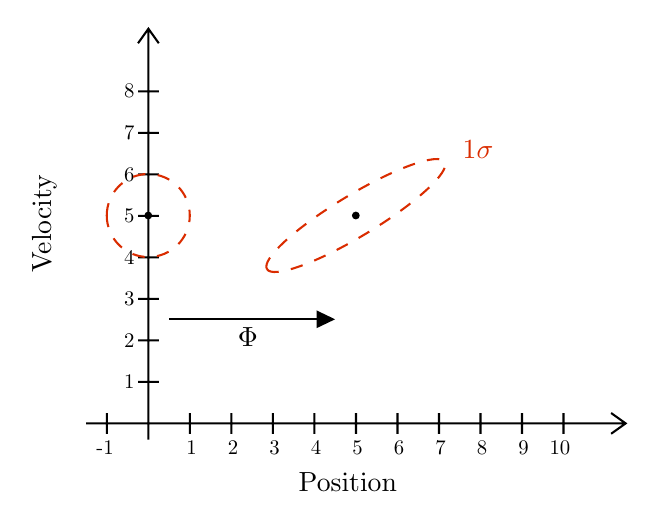
\begin{tikzpicture}[x=0.75pt,y=0.75pt,yscale=-1,xscale=1]
%uncomment if require: \path (0,300); %set diagram left start at 0, and has height of 300

%Shape: Axis 2D [id:dp5459576253225696] 
\draw  (180,230.15) -- (440,230.15)(210.07,40) -- (210.07,238) (433,225.15) -- (440,230.15) -- (433,235.15) (205.07,47) -- (210.07,40) -- (215.07,47) (230.07,225.15) -- (230.07,235.15)(250.07,225.15) -- (250.07,235.15)(270.07,225.15) -- (270.07,235.15)(290.07,225.15) -- (290.07,235.15)(310.07,225.15) -- (310.07,235.15)(330.07,225.15) -- (330.07,235.15)(350.07,225.15) -- (350.07,235.15)(370.07,225.15) -- (370.07,235.15)(390.07,225.15) -- (390.07,235.15)(410.07,225.15) -- (410.07,235.15)(190.07,225.15) -- (190.07,235.15)(205.07,210.15) -- (215.07,210.15)(205.07,190.15) -- (215.07,190.15)(205.07,170.15) -- (215.07,170.15)(205.07,150.15) -- (215.07,150.15)(205.07,130.15) -- (215.07,130.15)(205.07,110.15) -- (215.07,110.15)(205.07,90.15) -- (215.07,90.15)(205.07,70.15) -- (215.07,70.15) ;
\draw   (237.07,242.15) node[anchor=east, scale=0.75]{1} (257.07,242.15) node[anchor=east, scale=0.75]{2} (277.07,242.15) node[anchor=east, scale=0.75]{3} (297.07,242.15) node[anchor=east, scale=0.75]{4} (317.07,242.15) node[anchor=east, scale=0.75]{5} (337.07,242.15) node[anchor=east, scale=0.75]{6} (357.07,242.15) node[anchor=east, scale=0.75]{7} (377.07,242.15) node[anchor=east, scale=0.75]{8} (397.07,242.15) node[anchor=east, scale=0.75]{9} (417.07,242.15) node[anchor=east, scale=0.75]{10} (197.07,242.15) node[anchor=east, scale=0.75]{-1} (207.07,210.15) node[anchor=east, scale=0.75]{1} (207.07,190.15) node[anchor=east, scale=0.75]{2} (207.07,170.15) node[anchor=east, scale=0.75]{3} (207.07,150.15) node[anchor=east, scale=0.75]{4} (207.07,130.15) node[anchor=east, scale=0.75]{5} (207.07,110.15) node[anchor=east, scale=0.75]{6} (207.07,90.15) node[anchor=east, scale=0.75]{7} (207.07,70.15) node[anchor=east, scale=0.75]{8} ;
%Shape: Ellipse [id:dp9699291265749778] 
\draw  [color={rgb, 255:red, 218; green, 44; blue, 0 }  ,draw opacity=1 ][dash pattern={on 4.5pt off 4.5pt}] (190,130) .. controls (190,118.95) and (198.95,110) .. (210,110) .. controls (221.05,110) and (230,118.95) .. (230,130) .. controls (230,141.05) and (221.05,150) .. (210,150) .. controls (198.95,150) and (190,141.05) .. (190,130) -- cycle ;
%Shape: Ellipse [id:dp2897766336658041] 
\draw  [color={rgb, 255:red, 218; green, 44; blue, 0 }  ,draw opacity=1 ][dash pattern={on 4.5pt off 4.5pt}] (267.19,155.83) .. controls (264.33,151.1) and (281.19,135.7) .. (304.83,121.44) .. controls (328.48,107.17) and (349.96,99.44) .. (352.81,104.17) .. controls (355.67,108.9) and (338.81,124.3) .. (315.17,138.56) .. controls (291.52,152.83) and (270.04,160.56) .. (267.19,155.83) -- cycle ;
%Straight Lines [id:da46953353944392573] 
\draw    (220,180) -- (297,180) ;
\draw [shift={(300,180)}, rotate = 180] [fill={rgb, 255:red, 0; green, 0; blue, 0 }  ][line width=0.08]  [draw opacity=0] (8.93,-4.29) -- (0,0) -- (8.93,4.29) -- cycle    ;
%Straight Lines [id:da7890742663040001] 
\draw    (310,130) ;
\draw [shift={(310,130)}, rotate = 0] [color={rgb, 255:red, 0; green, 0; blue, 0 }  ][fill={rgb, 255:red, 0; green, 0; blue, 0 }  ][line width=0.75]      (0, 0) circle [x radius= 1.34, y radius= 1.34]   ;
%Straight Lines [id:da6149283693612637] 
\draw    (210,130) ;
\draw [shift={(210,130)}, rotate = 0] [color={rgb, 255:red, 0; green, 0; blue, 0 }  ][fill={rgb, 255:red, 0; green, 0; blue, 0 }  ][line width=0.75]      (0, 0) circle [x radius= 1.34, y radius= 1.34]   ;

% Text Node
\draw (281,252.4) node [anchor=north west][inner sep=0.75pt]    {Position};
% Text Node
\draw (152.4,159) node [anchor=north west][inner sep=0.75pt]  [rotate=-270]  {Velocity};
% Text Node
\draw (258,182.4) node [anchor=north] [inner sep=0.75pt]    {$\Phi $};
% Text Node
\draw (360,92.4) node [anchor=north west][inner sep=0.75pt]  [color={rgb, 255:red, 218; green, 44; blue, 0 }  ,opacity=1 ]  {$1\sigma $};


\end{tikzpicture}

    \caption{Time Update of Kalman Filter}
    \label{fig:Kalman Time Update}
\end{figure} 
Notice that the covariance ellipsoid changes shape from the initial circle to an elongated ellipse. In general, the ellipsoid will grow throughout time and the uncertainly in the position and velocity will increase until we get a measurement. When we get a new measurement, this ellipsoid will collapse to a smaller ellipsoid centered. We will now derive the measurement update equations in the predictor/smoother scheme.

\subsubsection{Measurement Update Equations}

\begin{comment}
One of the reasons for the development of the Kalman filter was because we cannot make perfect estimates of the state vector. Because this is the case, we include measurements of the states to make better estimates of them. The Kalman filter applies these measurements in an optimal manner in order to get the best estimate of the true nature of the system.

Measurements have uncertainties associated with them, so it makes sense for us to consider the accuracy of the measurement as compared to the accuracy of the state vector. Luckily, we have described both the measurement and the state vector uncertainties using the covariance!

Before we begin with the mathematics, I will describe a bit about the system we are modeling, which will make our lives a bit easier in conceptualizing the problem. Our situation is quite similar to the least squares estimate, as we want to extract an optimal estimate from some measurements. Our measurements are called $\bm{y}$, which are of the form:
$$\bm{y}=\begin{bmatrix}
    z_1\\z_2\\z_3\\\vdots\\z_m
\end{bmatrix}$$
Note that each element is not the same measurement at a different time, but rather a measurement of a different quantity. We are free to measure as many quantities of the system as we like. The number of measurements in the system is described by the value $m$.

The vector $\bm{x}$ is the familiar state vector, which has length $n$. Sometimes, our state vector is not in the same units as the measurements, or we only measure a few of the quantities from $\bm{x}$ in the measurements. For this reason, we include $H$ that ensures that $\bm{y}$ and $\bm{x}$ are of the same size and units. $H$ must therefore be of size $m\times n$.
\end{comment}

Our first goal for the measurement update is to understand how we can update the state after the measurement has occurred. We would like to know the \textit{posterior} distribution of the state (after measurement):
$$\hatx(n+1|n+1)$$
We can express this as a projection onto the current measurement space:
$$\hatx(n+1|n+1)=\mathcal{P}_{\mathcal{Y}_{n+1}}\bm{x}_{n+1}$$
This projection can once again be written in terms of the Gram-Schmidt projection:
$$\hatx(n+1|n+1)=\sum_{k=0}^{n+1}R_{\bm{x}_{n+1} \varphi_k} R_{\varphi_{k}}^{-1}\varphi_k$$
As we did in our previous derivation, we will split this sum into two components:
$$\hatx(n+1|n+1)=R_{\bm{x}_{n+1} \varphi_{n+1}} R_{\varphi_{n+1}}^{-1}\varphi_{n+1}+\sum_{k=0}^{n}R_{\bm{x}_{n+1} \varphi_k} R_{\varphi_{k}}^{-1}\varphi_k$$
We notice that the rightmost term is exactly the projection defined by$\hatx(n+1|n)=\mathcal{P}_{\mathcal{Y}_{n}}\bm{x}_{n+1}$ which is the \textit{prior} (before measurement) state $\hatx(n+1|n)$. The leftover term can be derived exactly like we did for the standard Kalman filter.

\begin{exercise}
Evaluate the term $R_{\bm{x}_{n+1} \varphi_{n+1}} R_{\varphi_{n+1}}^{-1}\varphi_{n+1}$ to find the closed form.
\end{exercise}

If you complete this derivation, you will find that our total answer is the following:
$$\hatx(n+1|n+1)=\hatx(n+1|n)+K_{n+1}\left[y_{n+1}-C\hatx(n+1|n)\right]$$
In the predictor/smoother model of the Kalman filter, we find that the total update is just the posterior state adjusted by the Kalman gain and innovation. This is very similar to our standard description. In fact, if we substitute in our equation for $\hatx(n+1|n)$, we get:
$$\hatx(n+1|n+1)=\Phi\hatx(n|n)+K_{n+1}\left[\bm{y}_{n+1}-C\hatx(n+1|n)\right]$$
Recall that our prior state estimate is defined as the projection of the future state onto past data: $\hatx(n+1|n) = \mathcal{P}_{\mathcal{Y}_n}\bm{x}_{n+1}$. Because the physical state propagates forward in time via the linear dynamics matrix $\bm{x}_{n+1} = \Phi \bm{x}_n$, we can use the linearity of the projection operator to pull $\Phi$ out completely:
\begin{equation}
\hatx(n+1|n) = \mathcal{P}_{\mathcal{Y}_n}(\Phi \bm{x}_n) = \Phi \mathcal{P}_{\mathcal{Y}_n}\bm{x}_n = \Phi \hatx(n|n)
\end{equation}
Now, substituting this directly into our measurement update equation at time step $n$ instead of $n+1$, we recover our original equation:
$$\hatx(n+1|n)=\Phi \hatx(n|n)+\Phi {K}_n\left[\bm{y}_n-{C}\hatx(n|n)\right]$$
We can see that the predictor/smoother scheme is not doing anything new, but the indices and equations will look slightly different. The predictor corrector scheme can be advantageous in code when we receive measurements at a lower rate than we update the state. We can loop over the standard update with $\hatx(n+1|n)=\Phi\hatx(n|n)$ until the measurement comes, at which point we incorporate the measurement innovation.

\subsubsection{Covariance Measurement Update}
Our final step is to update the covariance after receiving a new measurement in the system. As before, we can understand the covariance update by looking at the equation for the error covariance:
$$P(n+1|n+1)=\mathbb{E}[\bm{\tilde{x}}(n+1|n+1)\bm{\tilde{x}}(n+1|n+1)^*]$$

Our methodology will be the same as in the past. We will find $\bm{\tilde{x}}(n+1|n+1)$ by subtracting the true state from the estimated state. In the predictor/smoother model, this will look like:
\begin{align}
\tilde{\bm{x}}(n+1|n+1) &= \bm{x}_{n+1} - \hatx(n+1|n+1) \\
&= \bm{x}_{n+1} - \left( \hatx(n+1|n) + {K}_{n+1}\left[\bm{y}_{n+1}-{C}\hatx(n+1|n)\right] \right)
\end{align}
From here, we simply need to find the expectation of the outer product of this expression with itself. This is another good exercise to make sure we understand which components of the space are orthogonal to each other.

\begin{exercise}
Compute the expectation value for
$$\mathbb{E}[\bm{\tilde{x}}(n+1|n+1)\bm{\tilde{x}}(n+1|n+1)^*]$$
Using the fact that 
$$\tilde{\bm{x}}(n+1|n+1) =\bm{x}_{n+1} - \left( \hatx(n+1|n) + {K}_{n+1}\left[\bm{y}_{n+1}-{C}\hatx(n+1|n)\right] \right)$$
\end{exercise}
Like before, this expression will naturally lead us to a symmetric Joseph form after the appropriate cancellations:
\begin{equation}
{P}(n+1|n+1) = \left({I} - {K}_{n+1}{C}\right){P}(n+1|n)\left({I} - {K}_{n+1}{C}\right)^* + {K}_{n+1}{R}_{n+1}{K}_{n+1}^*
\end{equation}
As before, we typically implement this form of the equation because of its numerical stability. However, we can also simplify it to a Riccati form through some careful cancellation. Performing such a calculation (it is just matrix manipulations), we find:
\begin{equation}
{P}(n+1|n+1) = \left({I} - {K}_{n+1}{C}\right){P}(n+1|n)
\end{equation}
This is the last equation that we need for the predictor/smoother Kalman filter. We can combine all of the equations to get:
\begin{gather}
\color{boxBlue}\boxed{
\begin{array}{c}\color{black}
\bm{\hat{x}}({n+1|n)}=\Phi\bm{\hat{x}}(n|n)\\
\color{black}P(n+1|n)=\Phi_{n}P_n{\Phi_{n}}^T+Q_n
\end{array}
}\\
\color{boxBlue}\text{Prediction Step}\\
\color{boxBlue}\boxed{
\begin{array}{c}\color{black}
\hatx(n+1|n+1)=\hatx(n+1|n)+K_{n+1}\left[\bm{y}_{n+1}-C\hatx(n+1|n)\right]\\
\color{black} {P}(n+1|n+1) = \left({I} - {K}_{n+1}{C}\right){P}(n+1|n)
\end{array}
}\\
\color{boxBlue}\text{Measurement Update}
\end{gather}
As we finish this section, I will note that some authors prefer to use $+$ and $-$ symbols for the posterior and priors, respectively. This is not as explicit as the Bayesian notation, but it is often used in aerospace. The equations can be rewritten in this form as:
\begin{gather}
\color{boxBlue}\boxed{
\begin{array}{c}\color{black}
\bm{\hat{x}}_{n+1}^-=\Phi\bm{\hat{x}}_n\\
\color{black}P_{n+1}^-=\Phi_{n}P_n{\Phi_{n}}^T+Q_n
\end{array}
}\\
\color{boxBlue}\text{Prediction Step}\\
\color{boxBlue}\boxed{
\begin{array}{c}\color{black}
\hatx_{n+1}^+=\hatx_{n+1}^-+K_{n+1}\left[\bm{y}_{n+1}-C\hatx_{n+1}^-\right]\\
\color{black} {P}_{n+1}^+ = \left({I} - {K}_{n+1}{C}\right)P_{n+1}^-
\end{array}
}\\
\color{boxBlue}\text{Measurement Update}
\end{gather}
These are slightly more compact, so they can be appealing to use. However, I think the connection to Bayesian statistics and least squares estimation is important, and we should be reminded of that when writing our equations. It also helps to be explicit when filtering. Therefore, I'll prefer the first notation.

Finally, some authors choose to subtract 1 from all of the indices, such that the left side of the equation has index $n$ and terms on the right hand side have index $n-1$. I find this choice to be a bad choice and will not use such notation in this book. Unfortunately, it seems to be quite common in other literature and needs to be noted.

With the development of the predictor/smoother, we have developed all of the relevant ideas for the standard linear Kalman filter. The final sections of this chapter will investigate further extensions of the linear Kalman filter, such as adding a control signal or using a steady state version of the filter.


\section{Steady State Kalman Filtering}

In \autoref{chap: state space}, we saw that a properly designed observer will eventually converge to a steady state where the estimation error was zero. In that section, we did not assume that our system had noise affecting the state, but it will turn out that our Kalman filter will still reach a steady state so long as our noise matrices $(Q,R)$ are constant and our system is time-invariant. We will also require that the system is controllable and observable. When these conditions are met, our Kalman filter will converge to a steady state and we gain massive simplifications of the filter.

In this section, we will explore how we can derive the formula for the steady state Kalman filter. This will boast a huge increase in computational speed and a performance very similar to a standard linear Kalman filter in most cases. Even for systems that can be approximated as linear or will always operate in a equilibrium condition where a linearization is suitable, the steady state Kalman filter is often a very good choice for a lightweight filter that can run on almost any modern digital hardware.

\subsubsection{Deriving the Steady State Kalman Filter}
To derive the steady state Kalman filter, we consider the Riccati form of the covariance update equation:
$$P_{n+1}=\Phi P_n\Phi^*+Q_n-\Phi K_nCP_n\Phi^*$$
For the steady state filter, we require that the process noise in the system is constant such that $Q_n\rightarrow Q$. Additionally, the Kalman gain and covariance will all converge to steady values. The resulting equation is:
$$P=\Phi P\Phi^*+Q-\Phi KCP\Phi^*$$
We will write $K$ explicitly and place it in the equation:
\begin{gather}
K=PC^*(CPC^*+R)^{-1}\\
P=\Phi P\Phi^*+Q-\Phi PC^*(CPC^*+R)^{-1}CP\Phi^*
\end{gather}
This equation is a quadratic in the variable $P$ which we want to solve for. This equation is a discrete form of the Riccati equation explored in \autoref{chap: optimal control}. Since this equation has constant coefficients, it is \textit{algebraic}. As a result, we call this a \gls{dare}. While such equations can have many solutions, we are generally concerned with the stabilizing solution of $P$, which is unique. The \gls{dare} has a general form given by:
$$A^*XA-E^*XE-(A^*XB+S)(B^*XB+R)^{-1}(A^*XB+S)^*+Q=0$$
In Kalman filtering, we have a simplification of this general equation where $E=I$, $S=0$, $A=\Phi^*$, $X=P$, and $B=C^*$. We can solve such equations easily in MATLAB using the command \texttt{idare}. This will give the unique stabilizing solution to the equation. We may compute the matrix $P$ in MATLAB using this command:
\begin{matlabscript}{}
% the default idare takes A,B,Q,S,R,E
% these are Phi', C', Q, S=[], R, and E=[].
P = idare(Phi',C',Q,[],R,[]);
\end{matlabscript}
The derivation of the solution to the \gls{dare} is slightly advanced but is included in \autoref{sec:derivation of dare} in the Appendix. The derivation is a discrete time extension of the standard continuous time Riccati equation.

Once we have the steady state value of the error covariance matrix $P$, we can easily calculate the Kalman gain for the filter. The Kalman gain will be a constant matrix given by:
$$K=PC^*(CPC^*+R)^{-1}$$
In this formulation, we no longer require an explicit update of the error covariance matrix, and the Kalman filter can be collapsed into a simple state update:
$$\hatx_{n+1}=\Phi\hatx_n+\Phi K(\bm{y}_n-C\hatx)$$
For steady state filtering and some future endeavors, it will be useful to introduce an \textit{observer gain} $L$ which is simply defined as $\Phi K$. Under this new notation, we can combine the terms in $\hatx$ and write the steady state filter simply as:
\begin{gather}
\color{boxBlue}\boxed{
\begin{array}{c}\color{black}
\hatx_{n+1}=(\Phi-LC)\hatx_n+L\bm{y}_n\\
\color{black}L=\Phi PC^*(CPC^*+R)^{-1}
\end{array}
}\\
\color{boxBlue}\text{Steady State Kalman Filter}
\end{gather}
Note that $L$ is only required to be calculated once for systems satisfying the conditions described in this section.


\section{Steady State Filtering with Control}
Often we like to use the Kalman Filter with a state feedback controller. If we use a steady state filter, we can easily incorporate this into our controller. The more advanced case using a non steady-state filter will be explored at the end of this chapter.

The full state update equations are the same as before but include a control input:
\begin{align}
\bm{{x}}_{n+1}&=\Phi\bm{x}_n+\bm{w}_n+B\bm{u}_n\\
\bm{y}_n&=C\bm{x}_n+\bm{v}_n
\end{align}
To add control to the system, we formulate a state feedback controller. We may choose any method that yields a static feedback controller (like LQR or pole placement)\endnote{For a discrete time system, we would use the \texttt{dlqr} command in MATLAB.}. Here, our control will not be based on the true state $\bm{x}$ but rather the best estimate of the state:
$$\bm{u}_n=-K\hatx_n$$
Adding control only slightly augments our Kalman filter. In fact, the only thing that changes is $\hatx_{n+1}$. We now need to introduce the control to the system. Since the control signal passed into the system is a known input, we simply add it to the state estimate. We will use the matrix $L$ for the observer gain to avoid conflict with $K$ for the controller. This gives us the following for the state update (in a steady state filter):
$$\hatx_{n+1}=(\Phi-LC)\hatx_n+L\bm{y}_n+B\bm{u}_n$$
Since the additional control term appears identically in both the state estimate and the true state, the error state $\bm{\tilde{x}}$ remains the same as before. 
\begin{align}
&\quad\bm{{x}}_{n+1}=\Phi\bm{{x}}_{n}+\bm{w}_n+B\bm{u}_n
\\&-
\\&\quad\bm{\hat{x}}_{n+1}=\Phi \bm{\hat{x}}_{n}+ L(\bm{y}_n-C\bm{\hat{x}}_n)+B\bm{u}_n\\
&=\\
&\quad\bm{\tilde{x}}_{n+1}=\Phi\bm{\tilde{x}}_{n}+\bm{w}_n-L(C\bm{\tilde{x}}_{n}+\bm{v}_n)
\end{align}
As a result, the covariance update is unchanged and the rest of the Kalman filter is still the same as the standard Kalman filter. The covariance update can be written as:
\begin{align}
P_{n+1}&=\Phi P_n\Phi^*+Q_n- LCP_n\Phi^*
    \\
    L&=\Phi P_nC^*(CP_nC^*+R)^{-1}
\end{align}
From here we proceed in the exact same way to calculate $P$ and $L$, giving an identical result to the standard Kalman filter. Now, we can replace this term for the control input $\bm{u}_n$ and replace $\bm{y}_n=C\bm{x}_n+\bm{v}_n$:
\begin{align}
\bm{{x}}_{n+1}&=\Phi\bm{{x}}_{n}+\bm{w}_n-BK\hatx_n\\
\hatx_{n+1}&=(\Phi-LC-BK)\hatx_n+LC\bm{x}_n+L\bm{v}_n
\end{align}
Notice that both $\bm{x}$ and $\bm{\hat{x}}$ are linear in terms of $\bm{x},\hatx$ and the noise. Therefore, we can express the augmented state $\begin{bmatrix}
    \bm{x}&\hatx
\end{bmatrix}^T$ in terms of a linear state space model. This gives us:
$$\begin{bmatrix}
    {\bm{x}_{n+1}}\\
    {\hatx}_{n+1}
\end{bmatrix}=\begin{bmatrix}
    \Phi&-BK\\LC&\Phi-LC-BK\\
\end{bmatrix}\begin{bmatrix}
    {\bm{x}_n}\\
    {\hatx_n}
\end{bmatrix}+\begin{bmatrix}
    I&0\\0&L
\end{bmatrix}\begin{bmatrix}
\bm{w}_n\\\bm{v}_n
\end{bmatrix}$$
An example implementation of this filter will be given at the end of this chapter. An important thing to notice is that the dynamics of the true state are dependent on our estimate of the state. As a result, a poor estimate of the state could possibly destabilize the system. This is one argument that shows why introducing state estimation reduces the robustness of an LQR controller.


\section{Continuous and Hybrid Kalman Filters}

Often times, the models of our systems are developed as continuous models which we must then discretize in order to use the Kalman filter in digital systems. For such systems, it is sometimes useful to propagate the dynamics of the system using the continuous model directly. Since our measurements are very often still discrete, we can use a hybrid approach. Such a hybrid approach allows us to have continuous update of the state estimate and covariance with discrete measurement updates to the system.

Deriving the continuous Kalman filter rigorously is quite difficult and will not be done here.\endnote{Such a derivation requires measure theory, which is beyond the scope of the book.} We will consider a simple argument where we take the limit of the discrete Kalman filter as the timestep approaches zero. Let's remember that our discrete Kalman filter takes the form:
$$\bm{\hat{x}}_{n+1}=\Phi \bm{\hat{x}}_{n}+\Phi K_n(\bm{y}_n-C\bm{\hat{x}}_n)\\
\color{black}P_{n+1}=\Phi P_n\Phi^*+Q_n-\Phi K_nCP_n\Phi^*$$
Note that the time for the Kalman filter is given as $t=n\Delta t$. We can imagine reducing $\Delta t$ to increase $n$. In the limit as $\Delta t$ goes to zero, the following approximation of $\Phi$ becomes exact:
$$\Phi=(I+A\Delta t)$$
We can substitute this quantity in for $\Phi$ in the state estimate:
$$\bm{\hat{x}}_{n+1}=(I+A\Delta t) \bm{\hat{x}}_{n}+(I+A\Delta t) K_n(\bm{y}_n-C\bm{\hat{x}}_n)$$

\todo{Finish this}

For the continuous filter, we consider a continuous time state space:
\begin{gather}
    \bm{\dot{x}}(t)=A\bm{x}(t)+\bm{w}(t)\\
    \bm{y}(t)=C\bm{x}(t)+\bm{v}(t)
\end{gather}
As before, the noise terms are uncorrelated with each other. Additionally, the autocorrelation function for these noise terms takes the form of a Dirac delta:
$$\mathbb{E}[\bm{w}(t)\bm{\omega}(\tau)^*]=Q\delta(t-\tau)$$


This will give us our final result:
$$\dot{\bm{\hat{x}}}=A\hatx$$

\todo{finish}

\section{Unifying the LQR and Kalman Filter}
In our derivations of the Kalman Filter and the LQR controller, there were quite a few obvious parallels. In fact, they are so similar because of the duality between observability and controllability of a system. We can leverage this to unify the Kalman Filter and LQR controller into a single controller and observer, which we call the LQG system.

\todo{Finish this section}


\section{Kalman Filter Design Examples}
While it is important to be able to derive the various different Kalman filtering algorithms, using them in application is also very important. In this section, I will cover a few examples of Kalman filtering to make it evident how one might approach implementing the filter in real situations.

The following examples will use MATLAB/Simulink. Most of the results can be replicated in Python, but I am not aware of any simple replacement for Simulink. Most of the functionality can be replicated with code only, but Simulink design does prove to be useful for more complex models.

\subsubsection{MATLAB-Based Discrete Kalman Filter}
Let's consider a simple discrete time system modeling a mass spring damper. We can set up a simple state space as follows:
\begin{matlabscript}{State Space}
% set up the state space:
x0 = [1;2]; % initial pos, vel

A = [0 1;-1 -2]; % continuous transition

Phi = expm(A*0.1); % discrete transition
B = 0.1*[0;1]; % noise entering velocity channel
C = [1 1]; % measurement of pos + vel
D = 0.25*1; % noise in the measurement
\end{matlabscript}

Here, we use the $B$ and $D$ matrices to describe how the noise $\bm{w}$ and $\bm{v}$ will enter the system and to describe their magnitude. In this framework, the measurement noise covariance is given by $DD^*$ and the process noise covariance by $BB^*$. To initialize this filter, we require initial conditions on the state estimate and covariance matrix. We will also set up the noise for the system:
\begin{matlabscript}{Initial Conditions}
% number of samples to run
n = 0:1:80;

% come up with the random variables
z = numel(n);

w = 0.1*randn(z,1); % process noise
v = 0.25*randn(z,1); % measurement noise

xn = x0; % set the initial output as the x0 state

% set up state estimate:
x0_hat = [0;0];

x_hat_n = x0_hat; % set the initial estimate as the x0

q0 = [1 0;0 2]; % set the initial guess for the covariance
Qn = q0;   
\end{matlabscript}

Finally, we can run the Kalman filter for the system, which is basically just putting the appropriate equations into a for loop. Since we get measurements at every time step for this system, we can use the compact form of the equations here.
\begin{matlabscript}{Kalman Filter Loop}
% loop for KF:
for idx = 1:z

    % calculate the true state:
    xn_1 = Phi*xn + B*w(idx);

    % calculate the measurement:
    yn = C*xn + v(idx);

    % save these for the next step
    x(idx,:) = xn;
    xn = xn_1;

    % run the KF to estimate the state:
    delta = Phi*Qn*C'*inv(C*Qn*C' + D*D');
    x_hat_n_1 = Phi*x_hat_n + delta*(yn-C*x_hat_n);

    Qn_1 = Phi*Qn*Phi' + B*B' - Phi*Qn*C'*inv(C*Qn*C' + D*D')*C*Qn*Phi';

    % save these for the next step:
    x_hat(idx,:) = x_hat_n;
    x_hat_n = x_hat_n_1;
    Qn_out(:,:,idx) = Qn;
    Qn = Qn_1;
end
\end{matlabscript}

After running the filter, we can plot the outputs. For a well designed filter, we should expect that the state estimate converges towards the true estimate. Additionally, we should see that any errors in the estimate stay within the $1\sigma$ bounds most of the time. These results are shown in \autoref{fig:kf full linear} and \autoref{fig:kf error linear} and indicate expected performance of the Kalman filter.
\begin{figure}[ht]
    \centering
    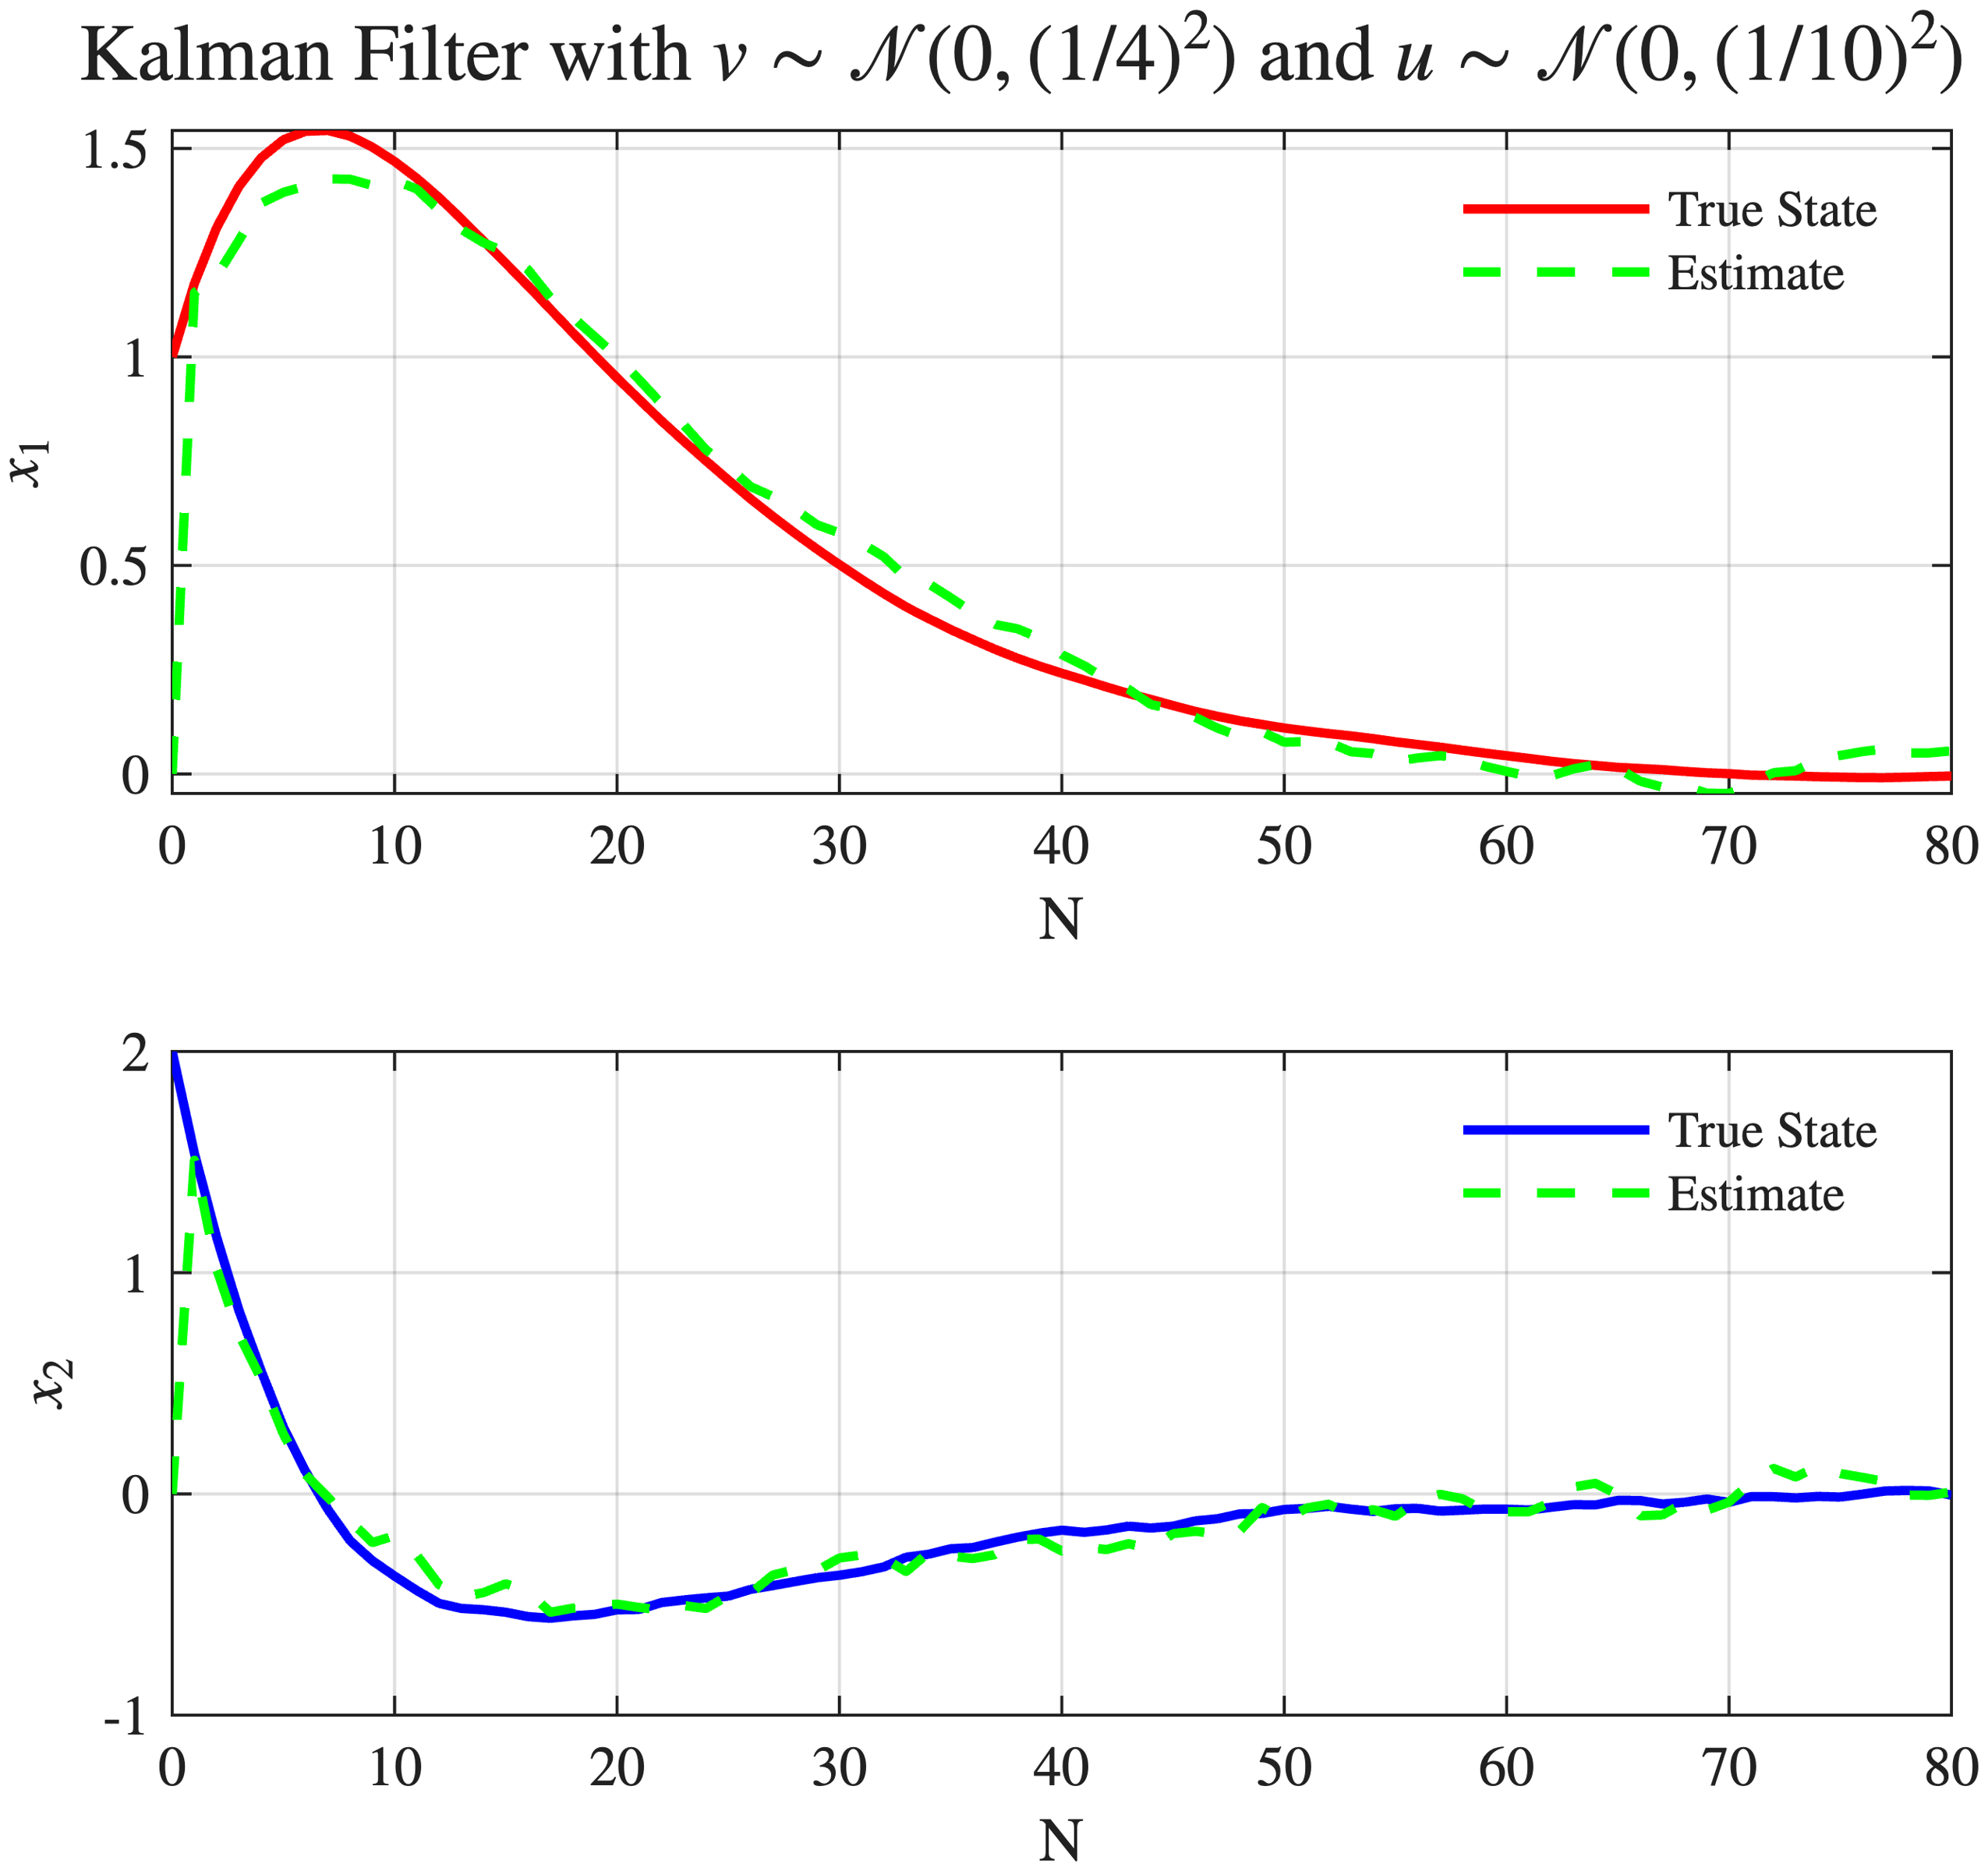
\includegraphics[width=.8\linewidth]{Images/KF_example1.png}
    \caption{True state of the system compared to the state estimate of the Kalman filter}
    \label{fig:kf full linear}
\end{figure}
\begin{figure}[ht]
    \centering
    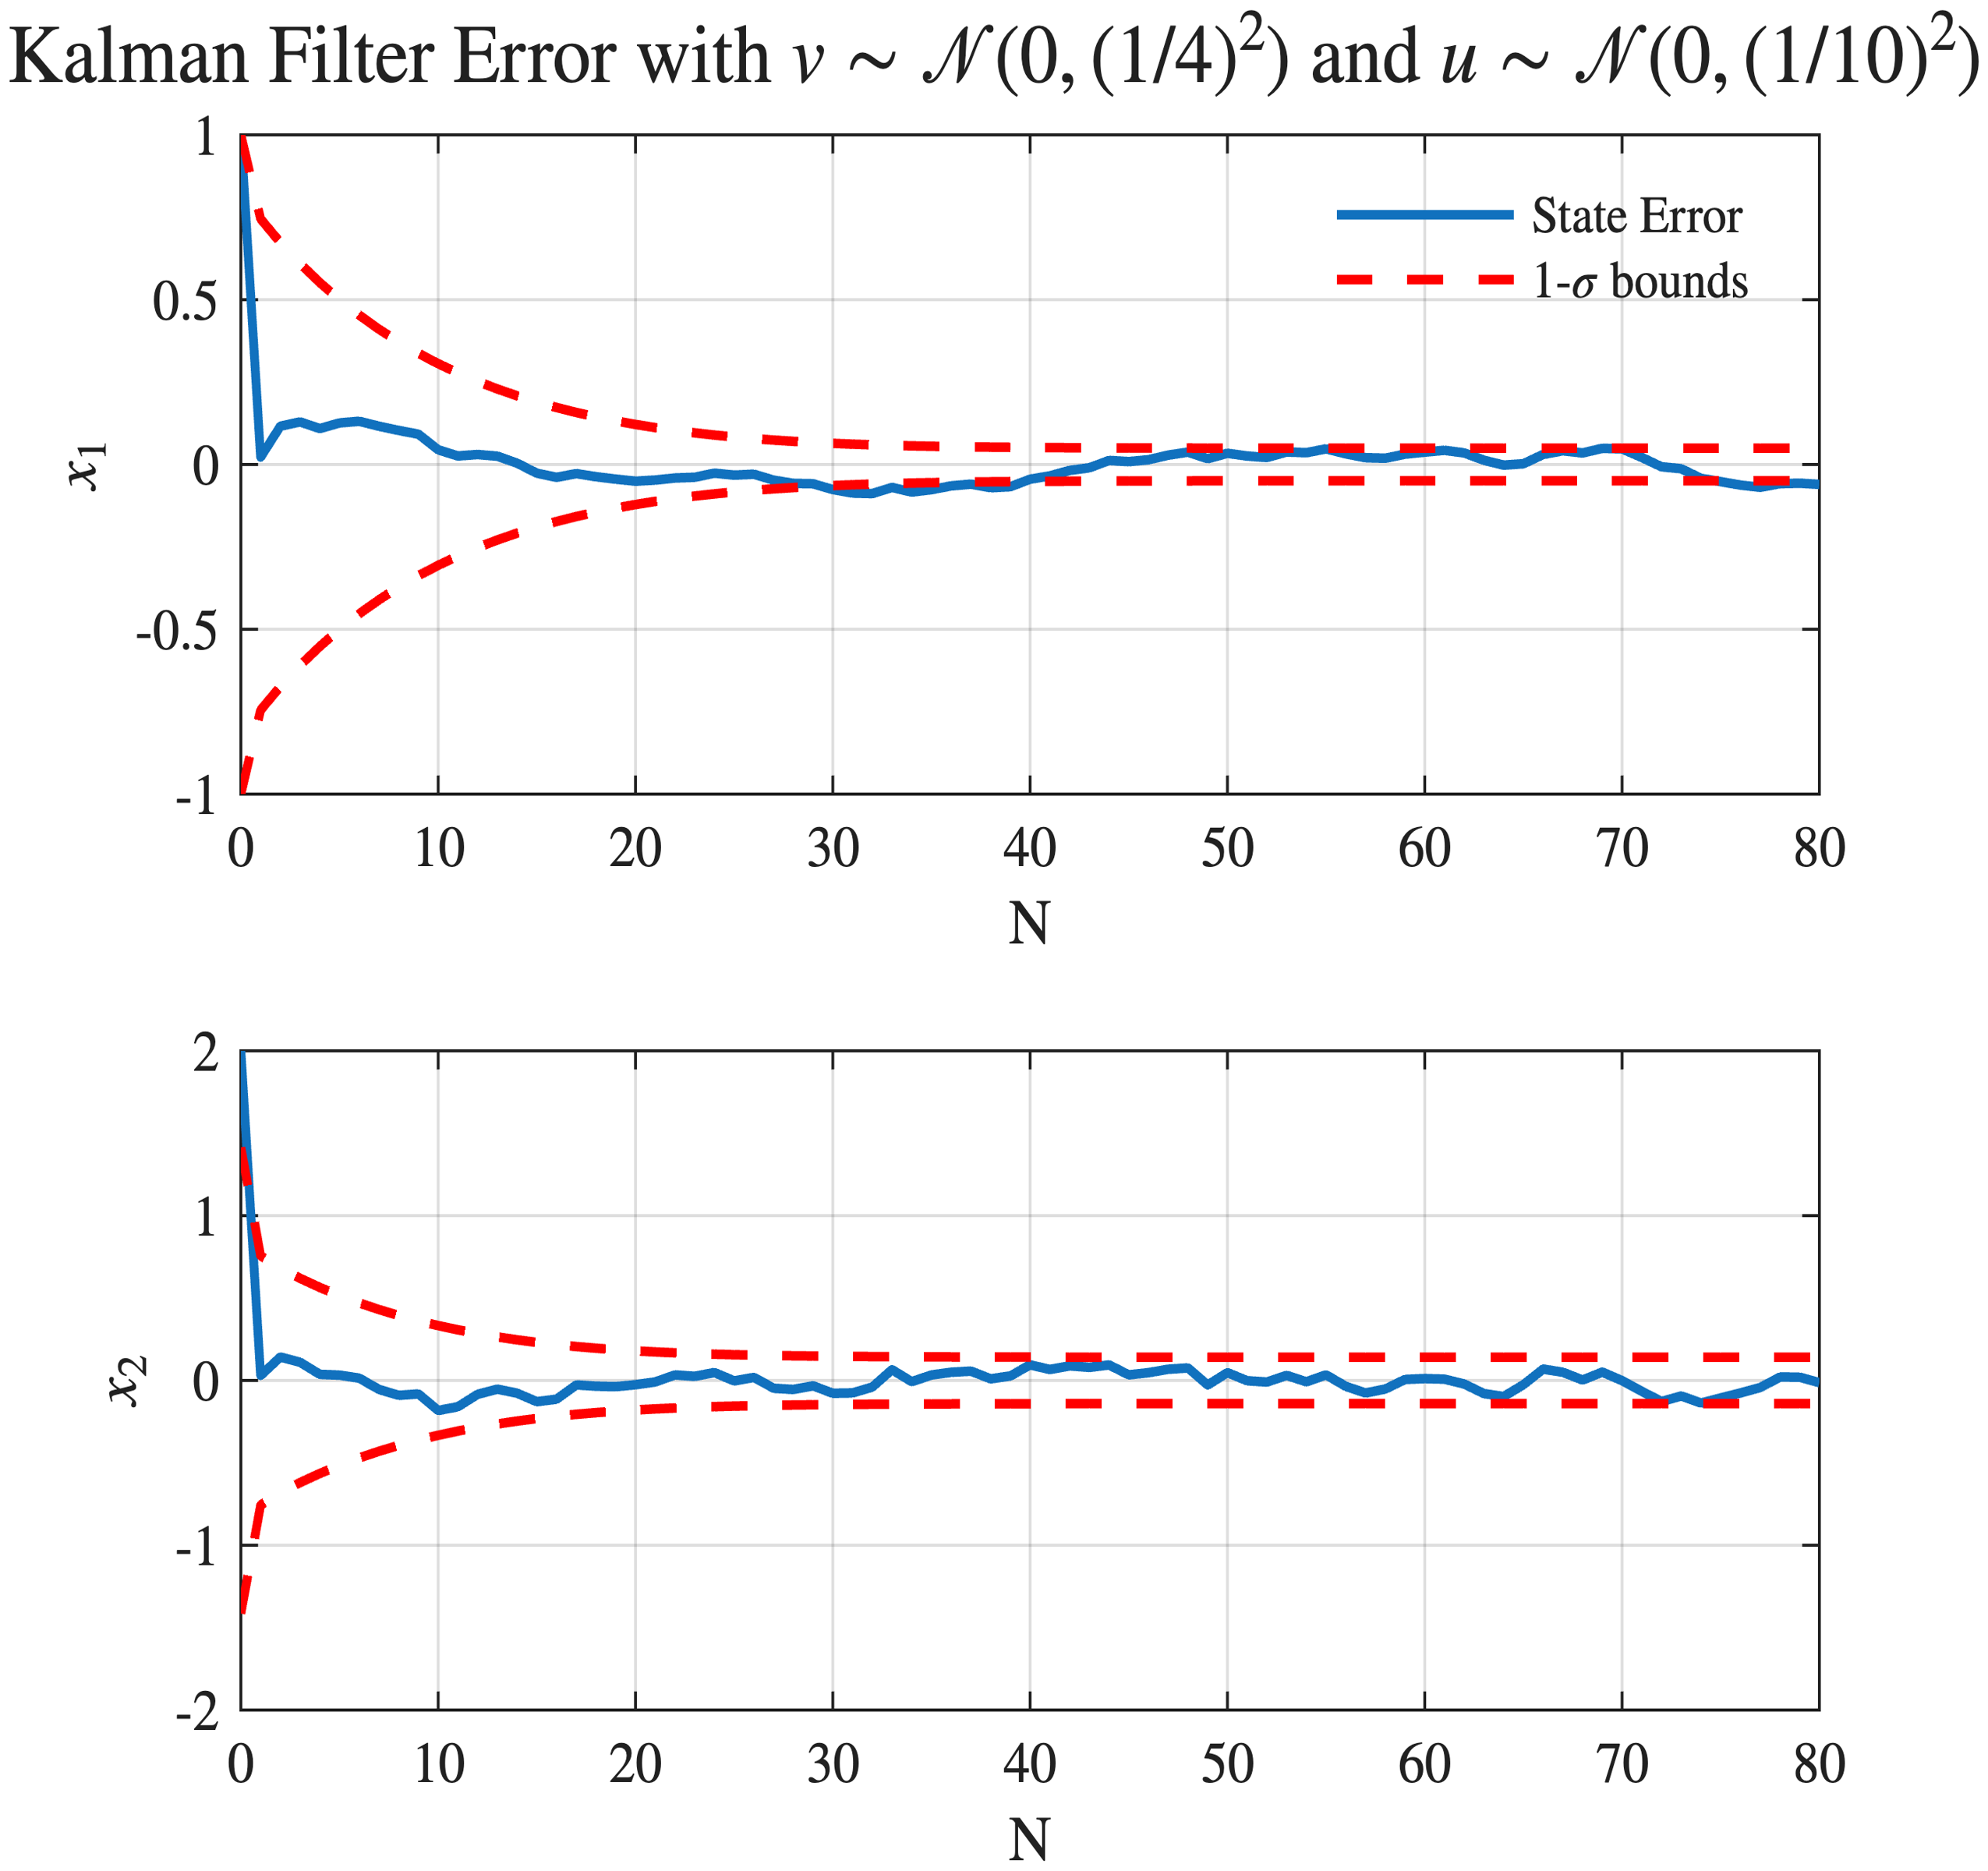
\includegraphics[width=.8\linewidth]{Images/KF_example2.png}
    \caption{Error in the state estimate of the Kalman filter with $1\sigma$ bounds (red dashed)}
    \label{fig:kf error linear}
\end{figure}
In typical analysis, we look at internal metrics of the filter because the true state of the system is not known. A common system metric is the measurement innovation of the filter at each step.


\subsubsection{Steady State Kalman Filtering}
For this problem, we will create a steady state filter for the discrete time system in the problem above to see the difference in performance (both computationally and in terms of filter outcomes). Since our state space is the same as the previous problem, we will only show the additions to the code. First, we establish the steady state Kalman gain of the system:
\begin{matlabscript}{}
% compute the steady state filter error covariance and Observer gain:
P = idare(Phi', C', B*B', D*D', [], []);
L = Phi*P*C'/(C*P*C' + D*D');
\end{matlabscript}
The loop for the computation of the new state estimate will be:
\begin{matlabscript}{}
% loop for KF:
for idx=1:z
    % calculate the true state:
    xn_1 = Phi*xn + B*w(idx);

    % calculate the meas:
    yn = C*xn + D*v(idx);

    % steady state KF:
    x_hat_n_1_steady  = (Phi-L*C)*x_hat_n_steady+L*yn;

    % save vars for plot
    x_hat_steady(idx,:) = x_hat_n_steady;

    % update vars for next step
    x_hat_n_steady = x_hat_n_1_steady;
    xn = xn_1;

end
\end{matlabscript}

We can compare the estimate of the steady state filter against the standard filter to see the difference. This is shown in \autoref{fig:steady}. We notice that the two estimates eventually become very close, with the steady state filter showing a different transient in the first 20-30 time steps. This result tells us that a good initial condition for $\bm{x}_0$ is more important for the steady state filter, as the transient response is fixed by the eigenvalues of $\Phi-LC$. Since the non steady filter can change the Kalman gain, convergence is often faster when initial conditions are unknown.
\begin{figure}[ht]
    \centering
    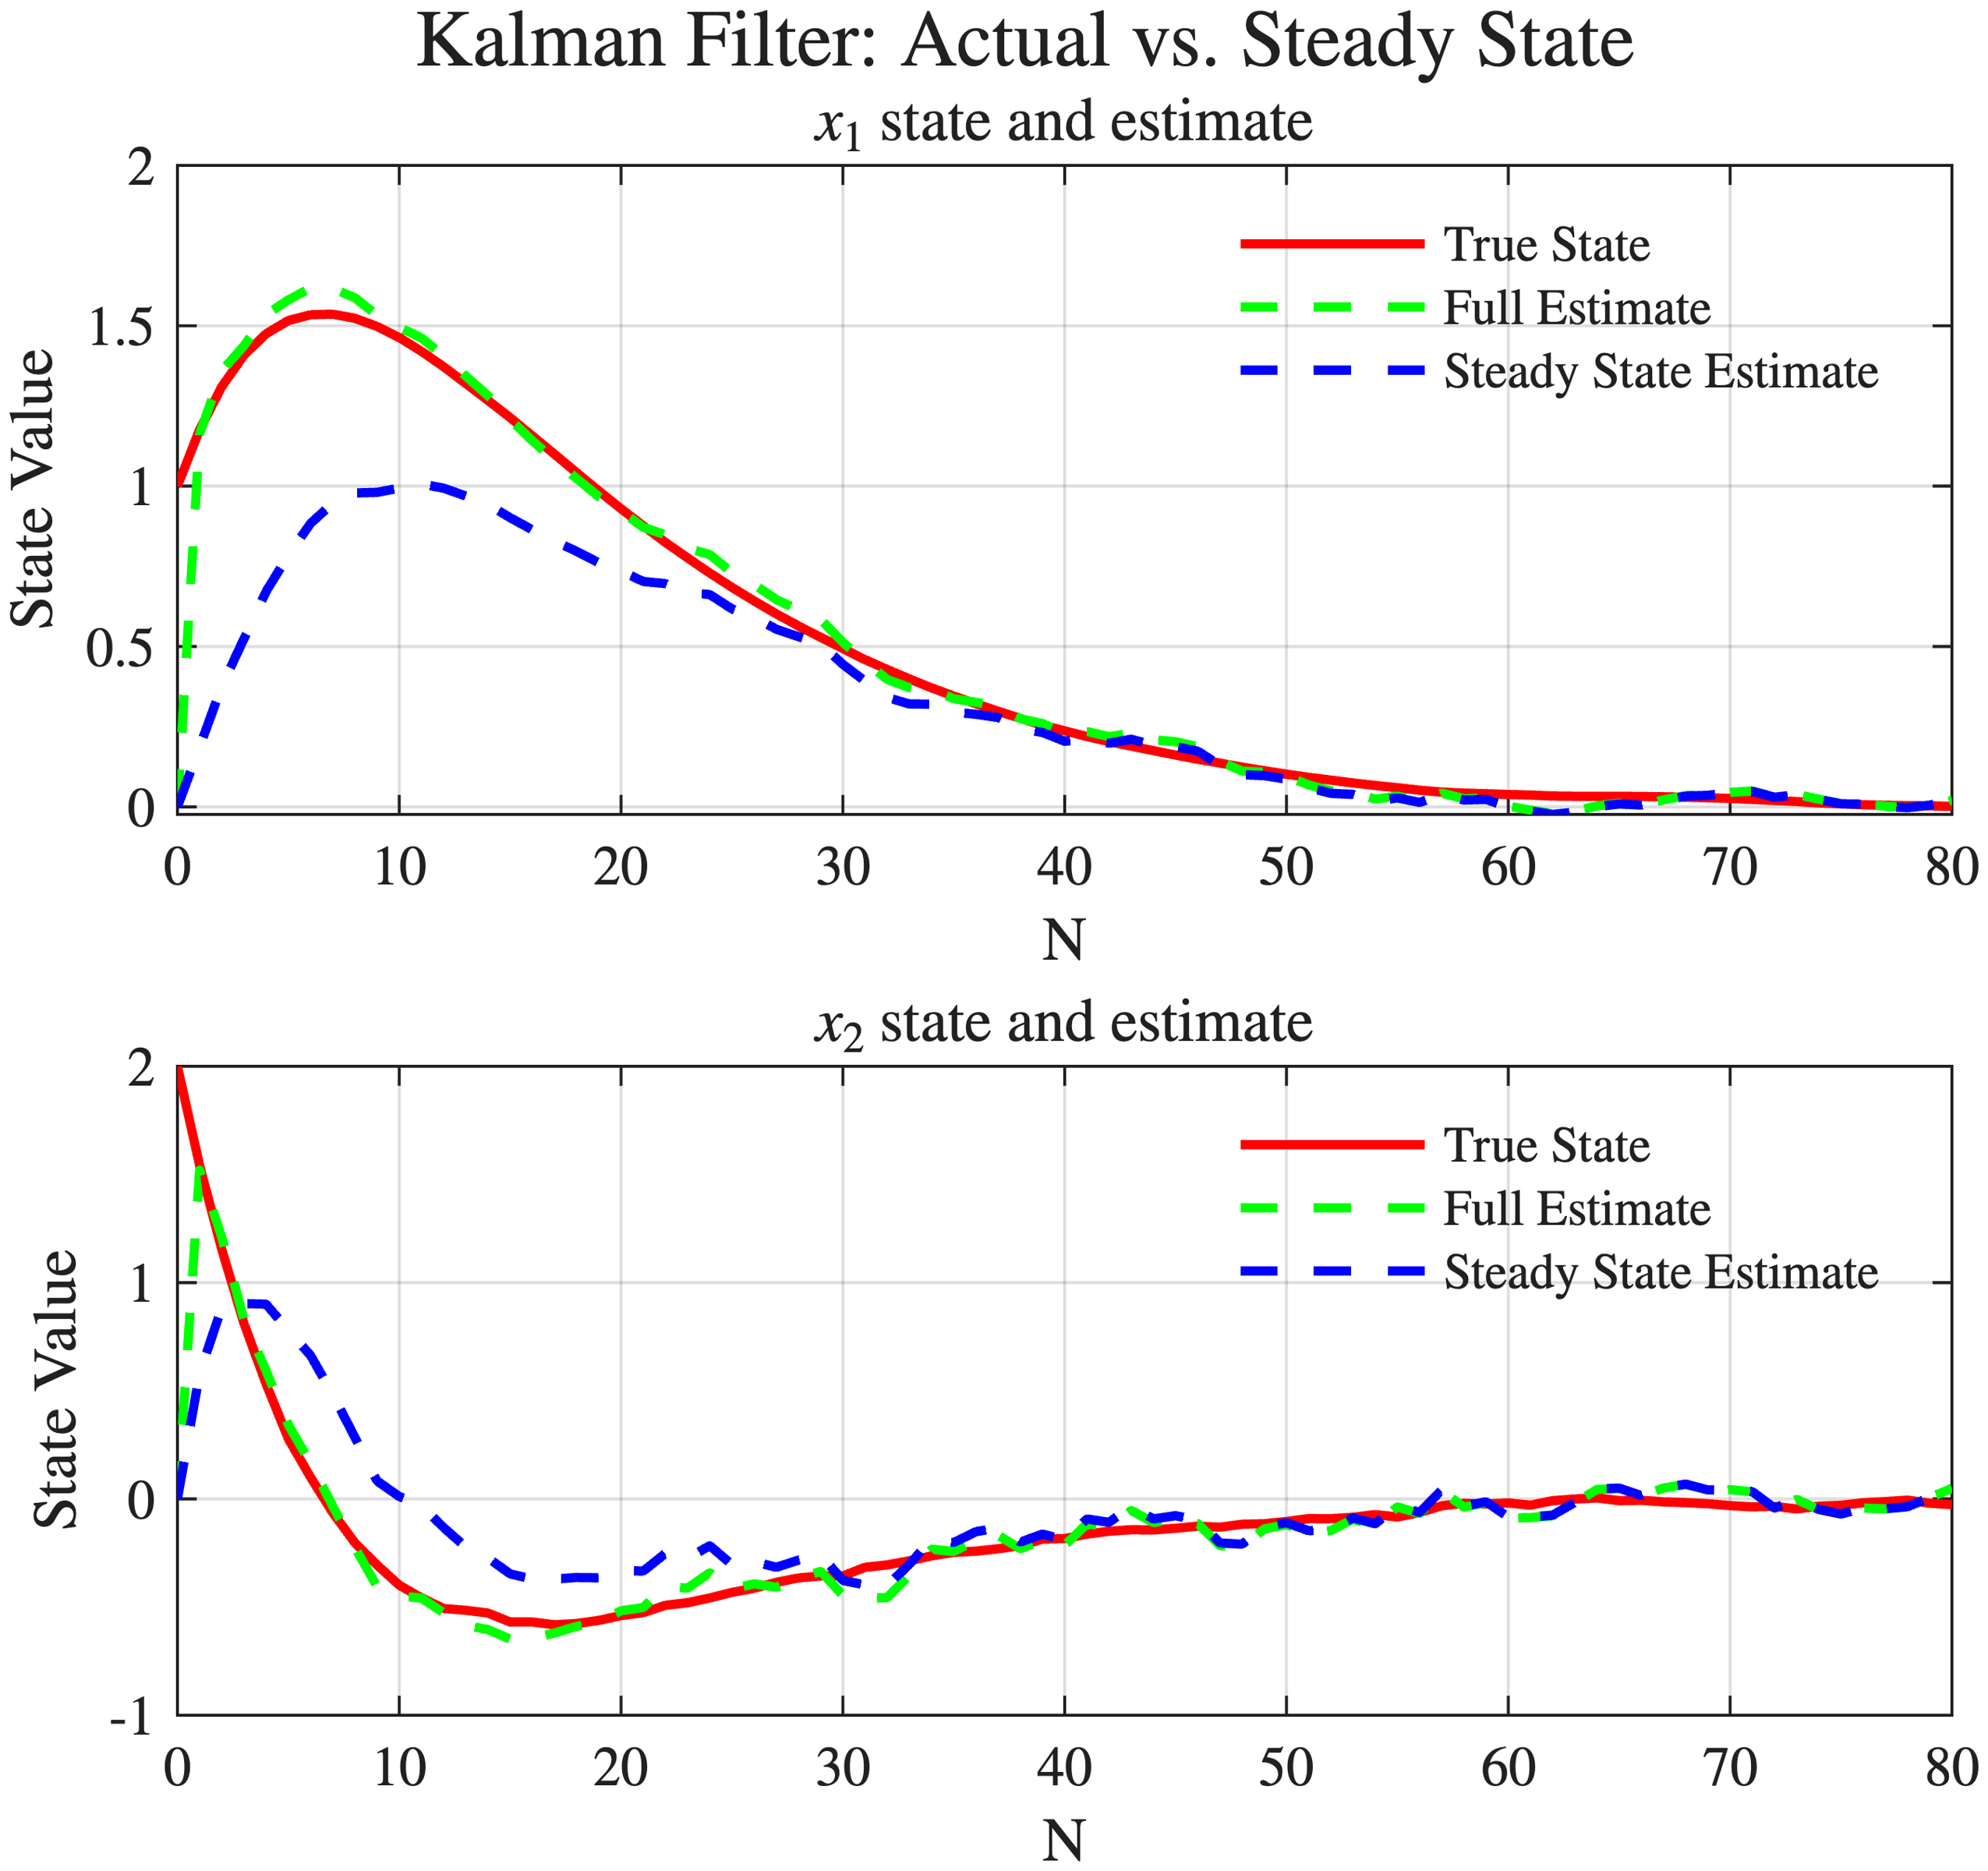
\includegraphics[width=1\linewidth]{SteadyFilter.png}
    \caption{Comparison of standard Kalman filter with the steady state Kalman filter}
    \label{fig:steady}
\end{figure}
For this $2\times2$ state space, the steady state filter computes its estimate in roughly one half to one third the time of the standard Kalman filter in MATLAB. Larger state spaces will benefit much more from the precomputation. Altogether, matrix inversions and multiplications in the standard filter create $\mathcal{O}(n^3+m^3)$ operations at each step (where $n$ is the size of the state $\bm{x}$ and $m$ the size of the measurement). For the steady state filter, we only need matrix multiplication and has time complexity of $\mathcal{O}(n^2+nm)$. We will see even greater improvements as the matrices become larger.


\subsubsection{Steady State Kalman Filtering with Control (Simulink)}


\newpage
\printendnotes


\chapter{Extensions of Kalman Filtering}\label{chap:kalman filter extensions}
In the development of the optimal estimator which resulted in the Kalman filter, we have made quite a few assumptions, some of which are quite limiting to its use. First and foremost is the assumption that our system must be linear. This, as it turns out, is the most egregious of the assumptions in the Kalman filter which most different approaches seek to resolve. There are several methods by which this can be resolved, each of which generates a variation of the Kalman filter with greater applicability to nonlinear systems. 

There are quite a few options to choose here, each with certain benefits and drawbacks for certain applications. Recent work has tended to favor the \gls{ukf} (\cite{wan_unscented_2000, chadha_unscented_2019}), but to understand that approach we must first look at the \gls{ekf} and related approaches.

There are other methods by which the state estimation can be achieved that are not related to the Kalman filter, such as the particle filter. While these can be quite useful, they fall outside the scope of this book and will not be discussed here.

To make this book practical, I want to provide real examples of each of these types of filters in MATLAB. Many times, there is a large gap between the practical application of these filters and the theory behind them. Although MATLAB has some built-in functionality for Kalman filtering, each situation -- particularly with the \gls{ekf} and \gls{ukf} -- can be quite unique and require a specialized implementation. It is best then, to understand code logic rather than being reliant on built-in functionality.

\section{The Extended Kalman Filter}

The \gls{ekf} is the first major extension of the Kalman filter.  In the \gls{ekf}, we use the concept of linearization in order to approximate a non-linear system as linear. In this way, we can apply the principles of Kalman filtering to a non-linear problem. At each point along our trajectory, we will linearize the dynamics of the system in order to propagate the state and the covariance. When we recieve measurement updates


\begin{example}[The 1D Radar Problem (Gelb)]
Do this later
\end{example}

\section{Trajectory Linearization}
One method that can be used that is less computationally expensive than the full \gls{ekf} is a method of `trajectory linearization'. This simplification may be used when we have prior information about the trajectory of the object. 

In this approach, we first construct a reference trajectory and apply linearization about the reference trajectory. Then, at every point in time, the reference trajectory linearization can be used for the kalman filter.

As an example, if we have some \gls{imu} data, we may propagate that data under the assumption that is perfect. This will give us a trajectory which is not perfect, but is good enough that it can inform our linearization model. We take a linearization at each point of this trajectory, and then we only have to match the result of the Kalman filter to this reference trajectory at each time.




\section{Multiplicative Kalman Filter}
The multiplicative Kalman filter is a special variety of the Kalman filter which is appropriate for systems which are non-linear but have a manifold description which is easily classified in terms of their \gls{lie algebra}. Often, rotations use the multiplicative Kalman filter because they fit this description exactly.

To see why we need the multiplicative Kalman filter, let us consider the problem of estimating the quaternion representation of the attitude of a vehicle. Our measurement update may look like:
$$\bm{q}^+=\bm{q}^-+K[\bm{y}-H\bm{q}^-]$$
One problem that can immediately be seen with this approach is that there is no enforcement of the quaternion magnitude. If the attitude errors are quite large, this can be quite a problem, and the enforcement of the quaternion magnitude needs to be performed elsewhere. This leads to the quaternion error update being less optimal than it otherwise would be.

One solution to counter this is to introduce a \textit{multiplicative} approach to the Kalman filter. Such an approach would maintain the quaternion magnitude constraint and prove useful in other parameterizations of the attitude representation.

\section{The Unscented Kalman Filter}
The unscented Kalman filter is another extension of the Kalman filter which is particularly useful in modeling systems which are highly non-linear in nature. The basic idea of the unscented Kalman filter is to make estimates for how the mean and covariance of the system change under the nonlinear dynamics of the system. If we are smart and pick a few points that model the distribution of the system well, we can track their evolution and reconstruct the change in the distribution.

The unscented Kalman filter relies on our knowledge used in deriving the Kalman filter. Let's briefly review the basics to see how we can implement them when our system is nonlinear.

Let's remember that we were able to define our state estimate in terms of the $R$ matrices as follows:
$$\bm{\hat{x}}=\mathcal{P}_\mathcal{M}\bm{x}=R_{xg}R_g^{-1}g$$
Here, we're going to define our $g$ as the following column vector:
$$g=\begin{bmatrix}
    1\\y-\mu_y
\end{bmatrix}$$
We can apply the standard formula for the state estimate. Let's first compute $R_g$:
$$R_g=\mathbb{E}gg^*=\mathbb{E}\begin{bmatrix}
1&y-\mu_y\\y-\mu_y&(y-\mu_y)^2
\end{bmatrix}=\begin{bmatrix}
    1&0\\0&\mathrm{Var}(y)
\end{bmatrix}$$
Now we compute $R_{xg}$:
$$R_{xg}=\mathbb{E}xg^*=\mathbb{E}x\begin{bmatrix}
    1&y-\mu_y
\end{bmatrix}=\begin{bmatrix}
    \mu_x&\text{Cov(x,y)}
\end{bmatrix}$$
If we multiply all these elements together, we will find that our state estimate is the following:
$$\bm{\hat{x}}=\begin{bmatrix}
    \mu_x&\text{Cov(x,y)}
\end{bmatrix}\begin{bmatrix}
    1&0\\0& \frac{1}{\mathrm{Var}(y)}
\end{bmatrix}\begin{bmatrix}
    1\\y-\mu_y
\end{bmatrix}=\mu_x+\frac{\text{Cov}(x,y)}{\text{Var}(y)}(y-\mu_y)$$
This form gives us an explicit connection between the $R$ matrices and the statistical values of the variance, covariance, and mean. If we can estimate each of these quantities, we can come up with a state estimate for our system.

\begin{exercise}
Remember that the error for a system is defined as:
$$e^2=\mathbb{E}(\bm{x}-\bm{\hat{x}})(\bm{x}-\bm{\hat{x}})^*=R_x-R_{xg}R_g^{-1}R_{xg^*}$$
Show that this can be written in terms fo the variance and covariance as:
$$e^2=\text{Var}(x)-\text{Cov}(x,y)\text{Var}(y)^{-1}\text{Cov}(y,x)$$
\end{exercise}

\subsection{The Unscented Transform}

\subsection{The Unscented Kalman Filter Algorithm}

\subsection{Examples of the UKF}

\newpage
\printendnotes



\chapter{Case Study: Inverted Pendulum}\label{chap:inverted pendulum}
The inverted pendulum is a classic problem in control theory, and for good reason! It demonstrates all of the basics of control theory, from derivation of \glspl{eom}, system linearization, and control design. With this problem, we can show a definitive example of many of the previous topics of discussion with a real application.

\begin{figure}[H]
    \centering
    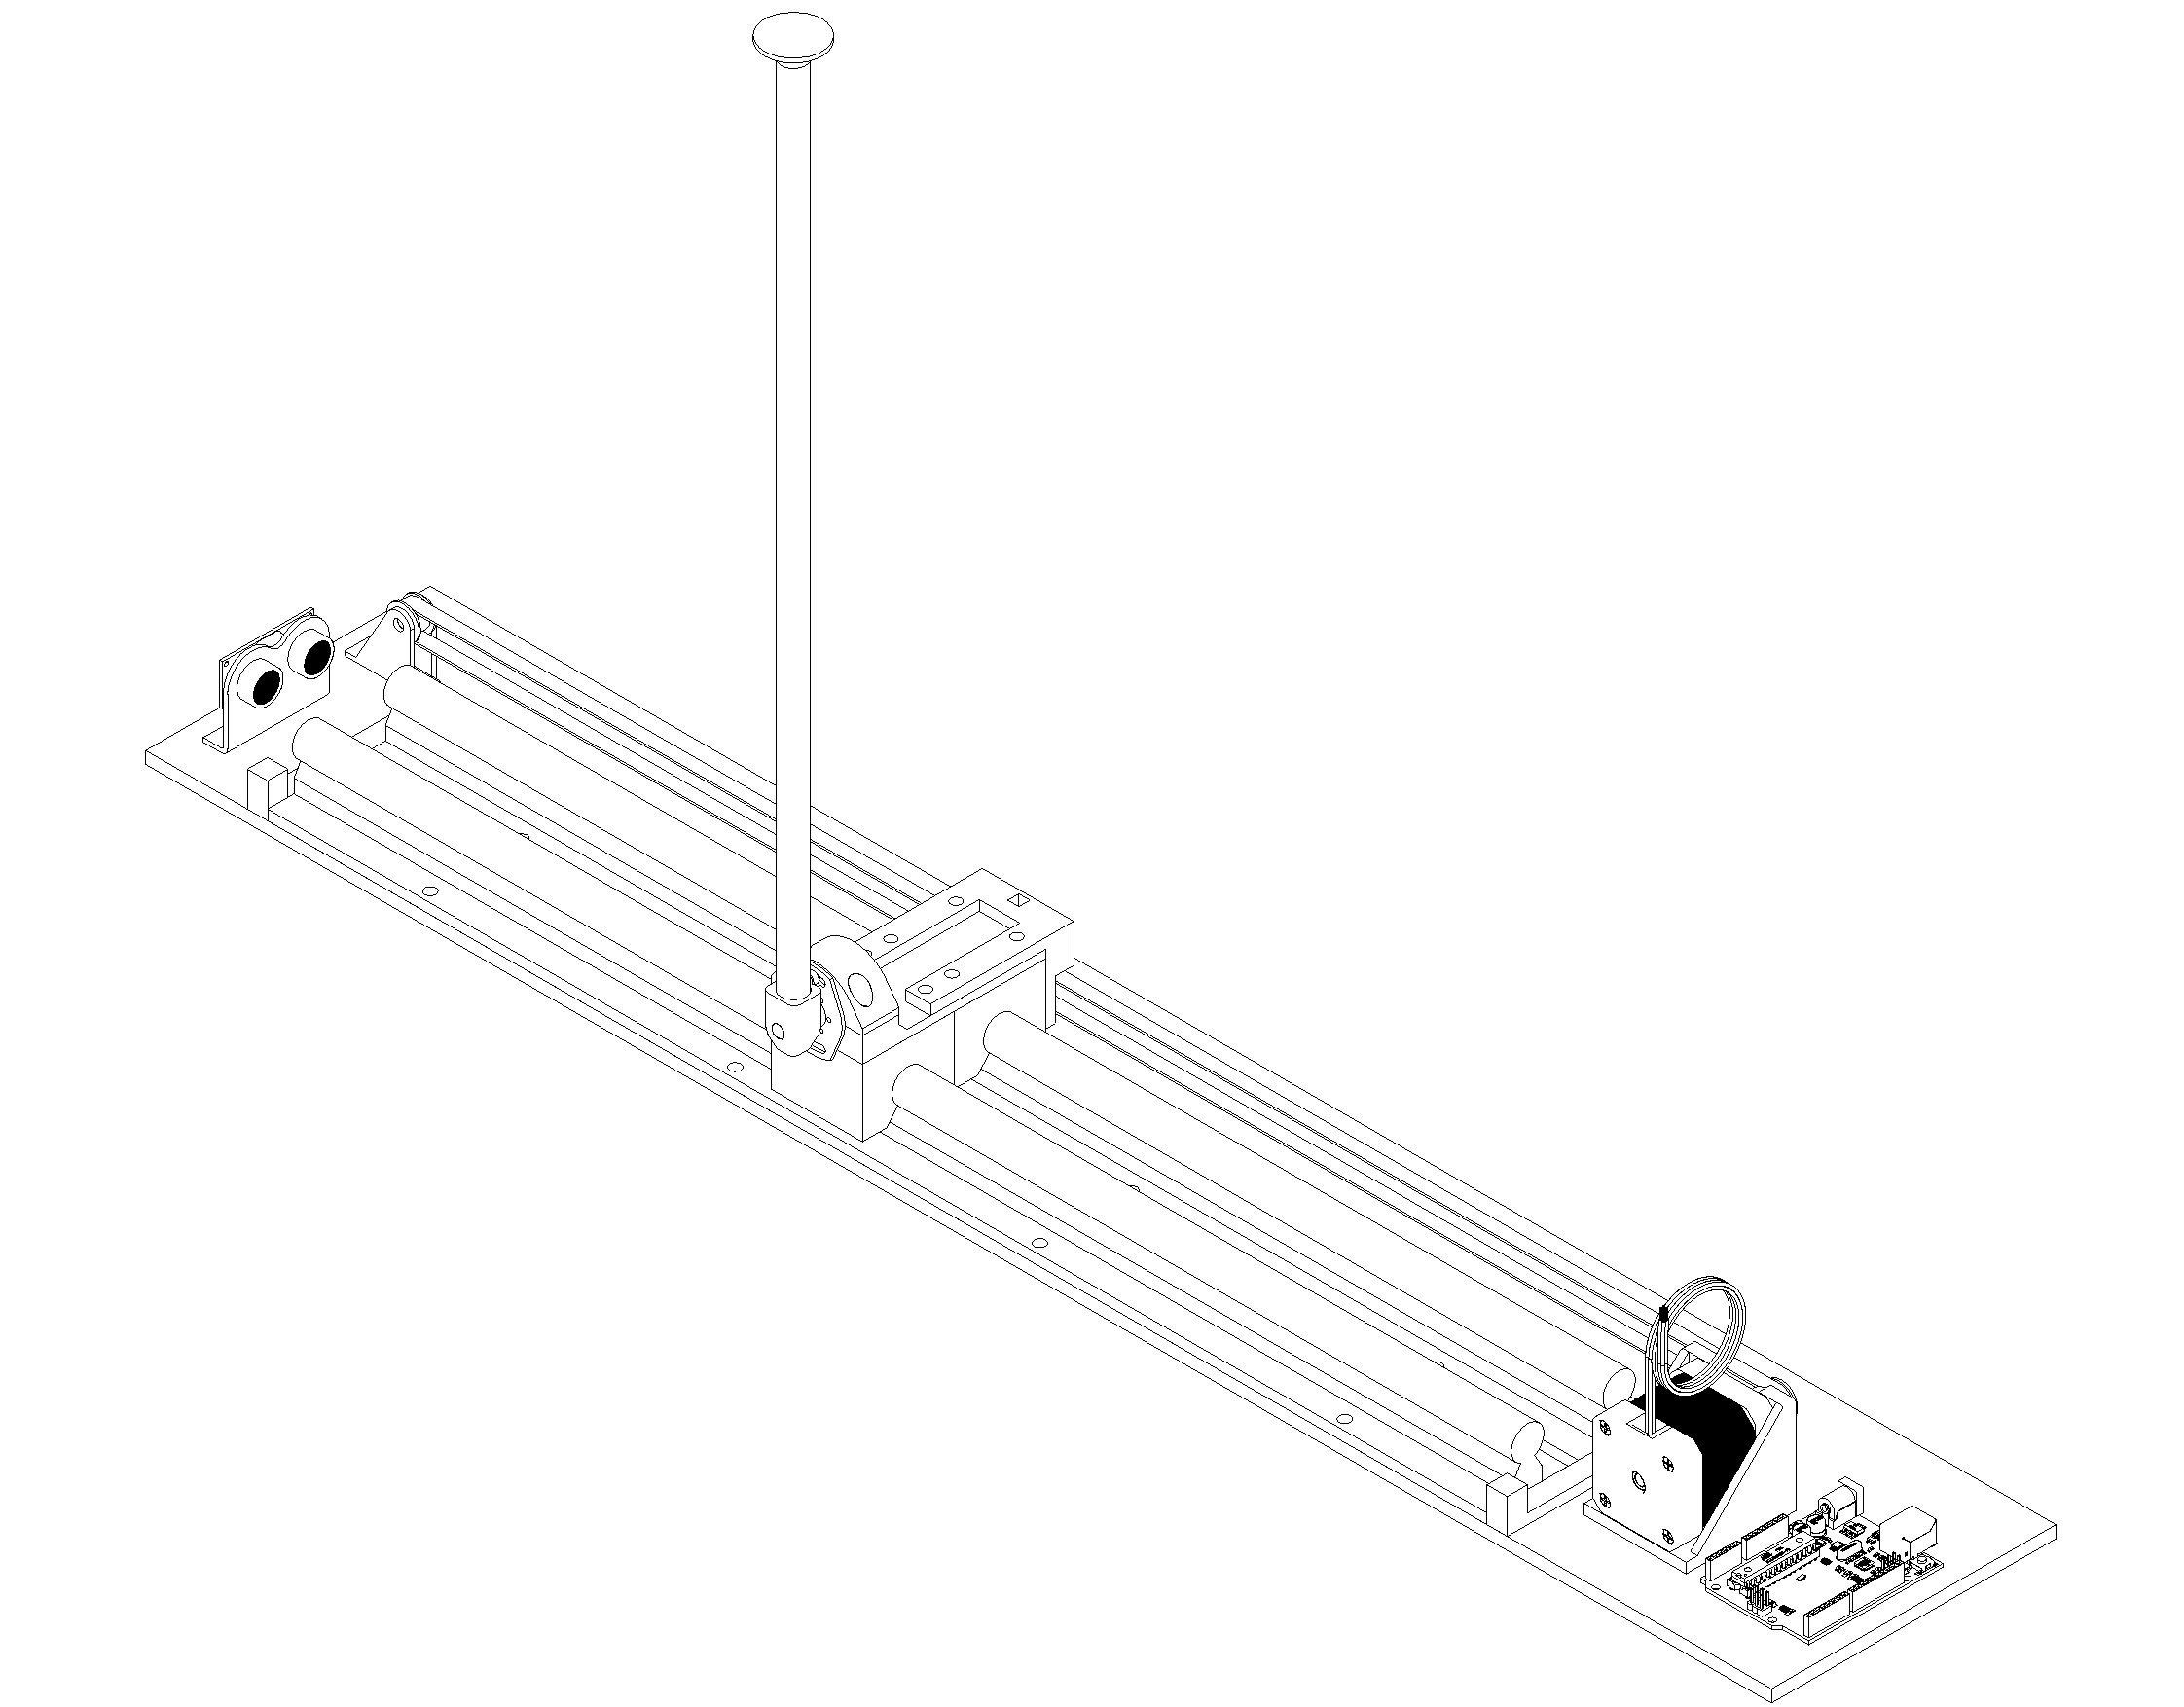
\includegraphics[width=.9\linewidth]{Images/InvertedPendulum.pdf}
    \caption{The Inverted Pendulum}
    \label{fig:inverted pend}
\end{figure}

At the end of this chapter, we will apply this controller to a real inverted pendulum system that I have built. My hope is that this will help demonstrate both the theory and practical application of the control theory concepts covered thus far. Additionally, some practical control applications will be discussed, such as the speed and torque control of DC motors.

\section{Equations of Motion}\label{sec:pend eom}
For any control system, we must understand the dynamics of the system that we want to control. For the simple inverted pendulum, this is quite easy to derive using energy mechanics.

Here, I will choose to use the \gls{Lagrangian} approach in the derivation, although the \gls{Hamiltonian} or Newtonian approach can also be taken. For this particular system, the \gls{Lagrangian} approach is quite simple and requires less knowledge of the forces acting on the system, which can become quite complicated! 

\subsubsection{Lagrangian Formulation}

We will consider a simple version of the pendulum-cart system, as shown in \autoref{fig:Pendulum Cart}.

\begin{figure}[ht]
    \centering



\tikzset{every picture/.style={line width=0.75pt}} %set default line width to 0.75pt        

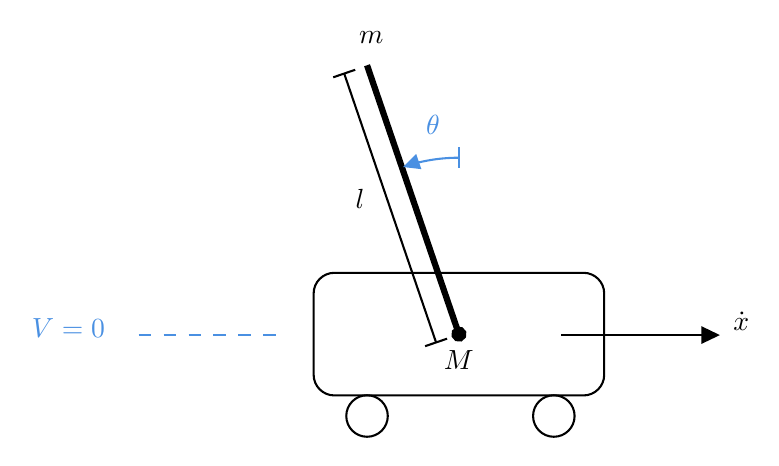
\begin{tikzpicture}[x=0.75pt,y=0.75pt,yscale=-1,xscale=1]
%uncomment if require: \path (0,300); %set diagram left start at 0, and has height of 300

%Shape: Rectangle [id:dp1823165404229382] 
\draw   (244.27,180) .. controls (244.27,174.48) and (248.75,170) .. (254.27,170) -- (374.27,170) .. controls (379.8,170) and (384.27,174.48) .. (384.27,180) -- (384.27,219.09) .. controls (384.27,224.61) and (379.8,229.09) .. (374.27,229.09) -- (254.27,229.09) .. controls (248.75,229.09) and (244.27,224.61) .. (244.27,219.09) -- cycle ;
%Straight Lines [id:da7877170508964265] 
\draw [line width=2.25]    (270,70) -- (314.27,199.55) ;
\draw [shift={(314.27,199.55)}, rotate = 71.13] [color={rgb, 255:red, 0; green, 0; blue, 0 }  ][fill={rgb, 255:red, 0; green, 0; blue, 0 }  ][line width=2.25]      (0, 0) circle [x radius= 2.14, y radius= 2.14]   ;
%Straight Lines [id:da5998055377665403] 
\draw    (363.64,200) -- (437,200) ;
\draw [shift={(440,200)}, rotate = 180] [fill={rgb, 255:red, 0; green, 0; blue, 0 }  ][line width=0.08]  [draw opacity=0] (8.93,-4.29) -- (0,0) -- (8.93,4.29) -- cycle    ;
%Shape: Arc [id:dp2580429075144265] 
\draw  [draw opacity=0] (287.33,119.03) .. controls (295.78,116.12) and (304.84,114.55) .. (314.27,114.55) -- (314.27,197.27) -- cycle ; \draw [color={rgb, 255:red, 74; green, 144; blue, 226 }  ,draw opacity=1 ]   (290.27,118.08) .. controls (297.87,115.78) and (305.93,114.55) .. (314.27,114.55) ; \draw [shift={(314.27,114.55)}, rotate = 180] [color={rgb, 255:red, 74; green, 144; blue, 226 }  ,draw opacity=1 ][line width=0.75]    (0,5.03) -- (0,-5.03)   ; \draw [shift={(287.33,119.03)}, rotate = 341] [fill={rgb, 255:red, 74; green, 144; blue, 226 }  ,fill opacity=1 ][line width=0.08]  [draw opacity=0] (8.04,-3.86) -- (0,0) -- (8.04,3.86) -- cycle    ;
%Shape: Circle [id:dp15264344475000924] 
\draw   (260,239) .. controls (260,233.48) and (264.48,229) .. (270,229) .. controls (275.52,229) and (280,233.48) .. (280,239) .. controls (280,244.52) and (275.52,249) .. (270,249) .. controls (264.48,249) and (260,244.52) .. (260,239) -- cycle ;
%Shape: Circle [id:dp05286140767854186] 
\draw   (350,239) .. controls (350,233.48) and (354.48,229) .. (360,229) .. controls (365.52,229) and (370,233.48) .. (370,239) .. controls (370,244.52) and (365.52,249) .. (360,249) .. controls (354.48,249) and (350,244.52) .. (350,239) -- cycle ;
%Straight Lines [id:da14376683390655187] 
\draw [color={rgb, 255:red, 74; green, 144; blue, 226 }  ,draw opacity=1 ] [dash pattern={on 4.5pt off 4.5pt}]  (160,200) -- (230,200) ;
%Straight Lines [id:da36211983725754393] 
\draw    (259,74) -- (303.27,203.55) ;
\draw [shift={(303.27,203.55)}, rotate = 251.13] [color={rgb, 255:red, 0; green, 0; blue, 0 }  ][line width=0.75]    (0,5.59) -- (0,-5.59)   ;
\draw [shift={(259,74)}, rotate = 251.13] [color={rgb, 255:red, 0; green, 0; blue, 0 }  ][line width=0.75]    (0,5.59) -- (0,-5.59)   ;

% Text Node
\draw (445,187.4) node [anchor=north west][inner sep=0.75pt]    {$\dot{x}$};
% Text Node
\draw (297,92.4) node [anchor=north west][inner sep=0.75pt]  [font=\normalsize,color={rgb, 255:red, 74; green, 144; blue, 226 }  ,opacity=1 ]  {$\theta $};
% Text Node
\draw (107,190.4) node [anchor=north west][inner sep=0.75pt]  [color={rgb, 255:red, 74; green, 144; blue, 226 }  ,opacity=1 ]  {$V=0$};
% Text Node
\draw (314.27,205.95) node [anchor=north] [inner sep=0.75pt]    {$M$};
% Text Node
\draw (272,52.4) node [anchor=north] [inner sep=0.75pt]    {$m$};
% Text Node
\draw (263,128.4) node [anchor=north west][inner sep=0.75pt]    {${l}$};

\end{tikzpicture}

    \caption{Pendulum-Cart System}
    \label{fig:Pendulum Cart}
\end{figure}
In this depiction, we will make quite a few simplifying assumptions, although some of these excluded dynamics can quite easily be recovered with a little effort:
\begin{itemize}
    \item The pendulum arm is assumed to originate at the center of mass of the cart.
    \item Friction and damping in the system is neglected, both in the rotation of the arm and the movement of the cart
    \item The reference for the potential energy is placed at the center of mass of the cart.
\end{itemize}

With these assumptions in place, we can apply the methods of \gls{Lagrangian} mechanics to derive the \glspl{eom} of the system. 

Starting with the \gls{Lagrangian} itself, we first define the generalized coordinates to use. In this case, the selection of $x$ and $\theta$ is quite obvious, as these two provide a minimal and simple realization of the system.

Since the motion of the system is non-obvious, it is best to employ the generalized equation for the kinetic energy in the derivation:
$$T=\frac{1}{2}\sum_im_i\left(\sum_j\frac{\partial\vec{r}_i}{\partial q_j}\dot{q}_j+\frac{\partial \vec{r}_i}{\partial t}\right)^2$$
There are two masses in the system, so the sum over $i$ includes both. We define the kinetic energy of the system as the sum of the kinetic energies of the cart ($i=1)$ and the pendulum ($i=2$). For the cart, only linear motion is permitted, so the kinetic energy is:
$$T_{cart}=\frac{1}{2}M\dot{x}^2$$
For the pendulum arm, both translational and rotational motion is permitted, so the total kinetic energy is more complicated. We will employ the formula above to find the kinetic energy in this case, considering only $i=2$ since $i=1$ has just been solved:
$$T_{pend}=\frac{1}{2}m\left(\sum_j\frac{\partial\vec{r}_2}{\partial q_j}\dot{q}_j+\frac{\partial \vec{r}_2}{\partial t}\right)^2$$
The vector $\vec{r}_2$ is expressed in terms of the two generalized coordinates, which gives 
$$\vec{r}_2=(x+l\sin\theta)\hat{\imath}+(l\cos\theta)\hat{\jmath}$$
One `trick' we can do in the computation that is sometimes simpler is to unexpand the chain rule and express the kinetic energy as:
$$T_{pend}=\frac{1}{2}m|\dot{r}_2|^2$$
Computing the value of $\dot{r}_2$ (remembering the implicit chain rule, now that we are not explicitly writing it), we have:
$$\dot{r}_2=(\dot{x}+l\cos\theta\dot{\theta})\hat{\imath}+(-l\sin\theta\dot{\theta})\hat{\jmath}$$
Performing the norm-square of $\dot{r}_2$ is the same as the dot product, so we square each element:
$$T_{pend}=\frac{1}{2}m\left[(\dot{x}+l\cos\theta\dot{\theta})^2+(-l\sin\theta\dot{\theta})^2\right]$$
Importantly, the computation of this gives a cross term from the expansion of the first term, which we may have missed otherwise. Altogether, $T_{pend}$ is:
$$T_{pend}=\frac{1}{2}m\dot{x}^2+\frac{1}{2}ml^2\dot{\theta}^2+ml\cos\theta\dot\theta\dot{x}$$
At this point, we can identify that the term $\frac{1}{2}ml^2\dot{\theta}^2$ is exactly the rotational kinetic energy of the rod. As a result, we can replace this term with $\frac{1}{2}I\dot{\theta}^2$. Finally, summing the two values of $i$ gives us the following kinetic energy for the system:
$$T_{cart}+T_{pend}=\frac{1}{2}\left[\left(M+m\right)\dot{x}^2+I\dot{\theta}^2\right]+ml\cos\theta\dot{\theta}\dot{x}$$

The potential is quite easy. For the cart, no potential exists because we have defined the potential at the center of mass to be $0$. For the arm, the potential is dependent on the angle, with the relationship given by:
$$V_{pend}=mgl\cos{\theta}$$
Altogether, this gives a \gls{Lagrangian} of the system as:
$$L=\frac{1}{2}\left[\left(M+m\right)\dot{x}^2+I\dot{\theta}^2\right]+ml\cos\theta\dot{\theta}\dot{x}-mgl\cos{\theta}$$
From here, we simply apply the Euler-Lagrange equations in both the $x$ and $\theta$ component directions.
\subsubsection{EOM Derivation}
Starting with the $x$-direction, we can directly apply the Euler-Lagrange equation with a generalized force to find the solution:
$$\frac{d}{dt}\left(\frac{\partial L}{\partial \dot{x}}\right)=\frac{\partial L}{\partial x}+F$$
Since $x$ itself has no presence in the equation,  $x$ is a cyclic coordinate in the solution. This directly implies linear momentum in the system is conserved by Noether's Theorem when no actuating forces are present. Additionally, this implies the RHS of the equation must be $F$ only. Considering the LHS then, we have:
$$\frac{d}{dt}\left(\frac{\partial}{\partial \dot{x}}\frac{1}{2}\left[\left(M+m\right)\dot{x}^2+I\dot{\theta}^2\right]+ml\cos\theta\dot{\theta}\dot{x}-mgl\cos{\theta}\right)$$
This simplifies quite quickly upon evaluation of the partial derivative to:
$$\frac{d}{dt}\left[\left(M+m\right)\dot{x}+ml\cos\theta\dot\theta\right]=F$$
Which is quite simply:
$$(M+m)\ddot{x}+ml\cos\theta\ddot{\theta}-ml\sin\theta\dot{\theta}^2=F$$
Next, we consider the $\theta$ component, which is quite a bit simpler. There is no generalized force in this component direction, so the result is:
$$\frac{d}{dt}\left(\frac{\partial L}{\partial \dot{\theta}}\right)=\frac{\partial L}{\partial \theta}$$
Starting again with the partial derivatives, we get the following (this time, there is no cyclic coordinate in $\theta$, implying angular momentum is \textit{not} conserved):
$$\frac{d}{dt}\left(I\dot{\theta}+ml\cos\theta\dot{x}\right)=mgl\sin\theta-ml\sin\theta\dot{\theta}\dot{x}$$
Once again, computation of the total derivative is quite simple and gives the following:
$$I\ddot{\theta}-ml\sin\theta\dot{\theta}\dot{x}+ml\cos\theta\ddot{x}=mgl\sin\theta-ml\sin\theta\dot{\theta}\dot{x}$$
Seeing that the $ml\sin\theta\dot{\theta}\dot{x}$ terms cancel, we are left with:
$$I\ddot{\theta}+ml\cos\theta\ddot{x}-mgl\sin\theta=0$$
Altogether, the full non-linear dynamics are described by:
\begin{gather}\label{eq:inverted pend eom}
\color{blue}\boxed{\color{black}
\begin{array}{c}
     (M+m)\ddot{x}+ml\cos\theta\ddot{\theta}-ml\sin\theta\dot{\theta}^2=F \\I\ddot{\theta}+ml\cos\theta\ddot{x}-mgl\sin\theta=0
\end{array}
}
  \\\color{blue}\mathrm{Inverted \ Pendulum \ EOMs}  
\end{gather}
\section{Linearization}
Linearizing the system is the next apparent step, as this will aid us in building a linear representation for our control algorithm. First, we must find the stationary points of the system. To find the stationary points of the system, we consider values of $x$ and $\theta$ such that the first derivatives are zero at that point. We also consider $F=0$, since we can produce an arbitrary $F$ to stabilize the system (as we will later do). It is for that reason we must consider $F=0$ when considering stable points of the system.

\subsubsection{Stationary points}

Since $x$ is not directly present in either equation, we are free to select any value of $x$ to produce a stable system. The physical interpretation is that the system can be stable for any horizontal position, which satisfies our intuition about the system. Considering $\theta$, we must select a value that satisfies:
$$\begin{array}{c}
     (M+m)\ddot{x}+ml\cos\theta\ddot{\theta}-ml\sin\theta\dot{\theta}^2=0 \\I\ddot{\theta}+ml\cos\theta\ddot{x}-mgl\sin\theta=0
\end{array}$$
All terms with $\ddot{x}$ can be eliminated since we have already shown that no positional dependence exists for the stationary points.  Thus, we have:
$$\begin{array}{c}
    ml\cos\theta\ddot{\theta}-ml\sin\theta\dot{\theta}^2=0 \\I\ddot{\theta}-mgl\sin\theta=0
\end{array}$$
We can recast this as a system of first order equations by considering $\omega=\dot{\theta}$, giving (after some simplification):
\begin{align}
     \omega^2&=\cot\theta\dot{\omega} \\
     \dot{\omega}&=\frac{g}{l}\sin\theta\\
     \omega&=\dot{\theta}
\end{align}
All that is left to do to find the stationary points is to consider the conditions on $\dot{\theta}$ and $\dot{\omega}$ such that they are 0. For $\dot{\theta}$, we simply have $\omega=0$ as the only possible stationary condition. Plugging $\omega$ back into the first equation (because all of them must be simultaneously satisfied at a stationary point), it is apparent that $\dot{\omega}=0$. This leaves us with the final equation, which is now\endnote{We could have similarly reached this conclusion by the fact that $\dot{\omega}$ must necessarily be zero at a stationary point by definition.}:
$$0=\frac{g}{l}\sin\theta$$
The solutions to this equation are $\theta=k\pi,\ k\in\mathbb{Z}$. In other words, the stationary points of the pendulum are $\theta=0$ and $\theta=\pi$, which correspond to the pendulum pointing directly up and down, respectively.

\subsubsection{Linearization}
When we control the pendulum system, a good control system will keep the pendulum close to the vertical upright position. For this reason, we can linearize the system about this upright position to attain an approximate linear solution.

All of the non-linear terms in the \gls{eom} derived in \eqautoref{eq:inverted pend eom} are nonlinear in $\theta$ as the result of trigonometric functions. Luckily, the linearizations for trigonometric functions are well known and easy to apply (these are better known by the name `small angle approximation'). Taking the first term of the Taylor series for each term about the $\theta=0$ condition yields the appropriate linearization:
\begin{align}
    \sin\theta&\approx\theta\\
    \cos\theta&\approx1
\end{align}
Additionally, the system linearization also ignores any terms of quadratic order or higher. It is for this reason that we can consider $\dot{\theta}^2\approx0$. Applying these three conditions, we have a linearization about the upright position:
\begin{align}\label{eq:linear pend}
     (M+m)\ddot{x}+ml\ddot{\theta}&=F \\I\ddot{\theta}+ml\ddot{x}-mgl\theta&=0
\end{align}
\subsection{State Space Representations}
With the linearized dynamics defined, we can quite easily create transfer functions for the system, as well as a state space realization. For each of these, it is best that we first separate the variables into decoupled equations of $\ddot{x}$ and $\ddot{\theta}$. We can start by solving the second equation in terms of $\ddot{\theta}$:

\begin{equation}\label{eq:theta double dot pend}
    \ddot{\theta}=\frac{mgl}{I}\theta-\frac{ml}{I}\ddot{x}
\end{equation}

Plugging \eqref{eq:theta double dot pend} into the first expression in \eqref{eq:linear pend}, the equation can be rearranged to:

$$\ddot{\theta}=\frac{mgl\theta-ml\ddot{x}}{I}$$
Now, we solve the two systems. The algebra is messy, but we may solve computationally in MATLAB:
\begin{matlabscript}{MATLAB}{}
syms theta x x_dot theta_dot theta_ddot ...
x_ddot g J M m F l

eqn1 = (M+m)*x_ddot + m*l*theta_ddot == F
eqn2 = J*theta_ddot + m*l*x_ddot - m*g*l*theta == 0

solution = solve([eqn1, eqn2], [x_ddot, theta_ddot])

solution.x_ddot

solution.theta_ddot
\end{matlabscript}

Which returns our solutions. We will write the denominator as $I(M+m)-(ml)^2=\Delta$ for the simplicity of writing. This gives us:
\begin{align}
    \ddot{x}&=\frac{FI-\left(ml\right)^2g\theta}{\Delta}\\
    \ddot{\theta}&=\frac{ml(Mg\theta+mg\theta-F)}{\Delta}
\end{align}

\subsubsection{State Space}
It is simplest to write the linear state space representation first. We consider the state vector as the generalized positions and velocities:
$$\bm{x}=\begin{bmatrix}
    x\\\dot{x}\\\theta\\\dot{\theta}
\end{bmatrix}$$
We can then write the state differential equation, $\dot{\bm{x}}=A\bm{x}+Bu$ using the equations above, where $F=u$:
\begin{gather}
    \begin{bmatrix}
    \dot x\\\ddot{x}\\\dot\theta\\\ddot{\theta}
\end{bmatrix}=\begin{bmatrix}
    0&1&0&0\\0&0&-\frac{(ml)^2}{\Delta}g&0\\
    0&0&0&1\\0&0&\frac{ml\left(Mg+mg\right)}{\Delta}&0
\end{bmatrix}\begin{bmatrix}
      x\\\dot{x}\\\theta\\\dot{\theta}
\end{bmatrix}+\begin{bmatrix}
    0\\\frac{I}{\Delta}\\0\\-\frac {ml}{\Delta}
\end{bmatrix}F,\quad\Delta=I(M+m)-(ml)^2
\end{gather}
The state space model is completed via the creation of $\bm{y}=C\bm{x}+Du$, the creation of which is quite simple. The states $x$ and $\theta$ are directly measured by sensors, so states 1 and 3 are observed. There is no direct input output relationship, so $D=0$. This gives:
$$C=\begin{bmatrix}
    1&0&0&0\\0&0&1&0
\end{bmatrix}$$
So that the full state space formulation is iven by:
\begin{gather}
    \begin{bmatrix}
    \dot x\\\ddot{x}\\\dot\theta\\\ddot{\theta}
\end{bmatrix}=\begin{bmatrix}
    0&1&0&0\\0&0&-\frac{(ml)^2}{\Delta}g&0\\
    0&0&0&1\\0&0&\frac{ml\left(Mg+mg\right)}{\Delta}&0
\end{bmatrix}\begin{bmatrix}
      x\\\dot{x}\\\theta\\\dot{\theta}
\end{bmatrix}+\begin{bmatrix}
    0\\\frac{I}{\Delta}\\0\\-\frac {ml}{\Delta}
\end{bmatrix}F,\quad\Delta=I(M+m)-(ml)^2\\
\bm{y}=\begin{bmatrix}
    1&0&0&0\\0&0&1&0
\end{bmatrix}\begin{bmatrix}
      x\\\dot{x}\\\theta\\\dot{\theta}
\end{bmatrix}
\end{gather}

% \subsubsection{Transfer Function}
% The transfer function for the linearized system is also quite plain to express (in fact, we cannot write the transfer function for a non-linear system). We start by considering the \gls{laplace transform} of \eqautoref{eq:linear pend}:
% \begin{align}
%     (M+m)s^2X(s)-mls^2\Theta(s)=F(s)\\
%     Is^2\Theta(s)-mls^2X(s)-mgl\Theta(s)=0
% \end{align}
% The problem is mostly algebraic manipulation at this point to separate the system into equations which contain $X(s)$ and $\Theta(s)$ separately. This is accomplished by the usual means of solving for two variables. Doing so gives:
% $$\frac{\Theta(s)}{F(s)}=\frac{ml}{(M+m)[s^2(I-m^2l^2)-mgl]}$$
% $$\frac{X(s)}{F(s)}=\frac{s^2I-mgl}{s^2(M+m)(s^2I-s^2m^2l^2-mgl)}$$

% These transfer functions are not particularly useful in this application, as they inherently define \gls{siso} relationships. Because we want to control several aspects of the pendulum motion simultaneously (the angle, position, and their derivatives), the transfer functions are less useful. For the rest of this chapter, I will prefer to use the state space model rather than the transfer functions when discussing the system dynamics.

\subsubsection{State Space with Damping}
One assumption made earlier in the modeling of the system is that the system is frictionless. To improve the modeling to some degree, we can introduce a term with a dependence on the velocity and angular velocity. This model of friction is quite simply, but can easily be incorporated into the model. For a standard second-order system, it is quite typical to denote drag or damping with a term linearly dependent on the velocity -- that is, $c\dot{x}$. We can easily incorporate this in the state space model, denoting the damping on the cart $c$ and the damping on the pendulum as $d$:

\begin{gather}
    \begin{bmatrix}
    \dot x\\\ddot{x}\\\dot\theta\\\ddot{\theta}
\end{bmatrix}=\begin{bmatrix}
    0&1&0&0\\0&c&-\frac{(ml)^2}{\Delta}g&0\\
    0&0&0&1\\0&0&\frac{ml\left(Mg+mg\right)}{\Delta}&d
\end{bmatrix}\begin{bmatrix}
      x\\\dot{x}\\\theta\\\dot{\theta}
\end{bmatrix}+\begin{bmatrix}
    0\\\frac{I}{\Delta}\\0\\-\frac {ml}{\Delta}
\end{bmatrix}F,\quad\Delta=I(M+m)-(ml)^2\\
\bm{y}=\begin{bmatrix}
    1&0&0&0\\0&0&1&0
\end{bmatrix}\begin{bmatrix}
      x\\\dot{x}\\\theta\\\dot{\theta}
\end{bmatrix}
\end{gather}

The inclusion of these terms is best left as an `engineering judgment`. If these terms can be well characterized or estimated, they should likely be included. They may, however, actually reduce the accuracy of the model. In my implementation, I have chosen to neglect these terms and have little issue doing so.

\subsection{Controllability and Observability}
As has been previously noted, the controllability of the system is dependent on $A$ and $B$ and the observability on $A$ and $C$. We can find the controllability and observability of the system quite easily through application of the previously mentioned formulas.

The easiest method to do so is through the use of the MATLAB commands:
% add matlab commands
As we can see, the system is fully controllable and observable, which is good news! This means that a \gls{lqr} controller will work well in this application.
% to do

\section{LQR Control}
\subsubsection{Why LQR?}
For the pendulum, an \gls{lqr} controller is chosen. Why choose a \gls{lqr} controller over a simpler controller such as \gls{pid}?

The main reason to do so is because we want to control both the position and the angle of the pendulum. Since our track has a limited length, we need to force the $x$ position back towards 0. This is perfect for the \gls{lqr} controller, which is naturally a \gls{mimo} controller. If we were to use \gls{pid} for the control, we would need two separate controllers, one which controls the angle, and another which controls the position. The fact that \gls{pid} is \gls{siso} only is one of the big drawbacks of \gls{pid} control scheme!

One obvious drawback of the \gls{pid} implementation is that the two controllers will `fight' each other. One controller may decide that positioning the cart is more important than maintaining the upright angle, and the pendulum will fall over.

A less obvious drawback is that the \gls{pid} controller is acting without the knowledge of the system dynamics. The consequence of this is that the \gls{pid} will only measure the angle, and apply a force in such a way to minimize this. However, without knowledge of the system dynamics, the PID controller would need very high gains to maintain control of the system. In a real system, large gains manifest themselves as excessively large control commands and instabilities. These are downsides which make the \gls{pid} controller a very poor choice for this application.

All of this is to say that the choice of the \gls{lqr} controller is quite justified in this situation. The selection of the \gls{lqr} controller does introduce some additional design criteria. First and foremost, the \gls{lqr} controller requires that the system has knowledge of the full state. Since we have full observability in the system, this is not an issue. As we will see in the real implementation, however, some of these states which are very well observable in theory often have lots of noise or other challenges in their implementation.

This noise can be dealt with in various ways, some of which will be explored later. One obvious option is to implement a Kalman filter for state estimation, but this can be computationally expensive for low end hardware such as the Arduino Uno.

\subsubsection{LQR Considerations}

The \gls{lqr} controller 


\section{Motor Control}
Before we get into the real implementation of the pendulum, we must discuss the topic of motor control. The pendulum, and many other control systems that we would like to build, are reliant on motors of many types. This section will not be an exhaustive listing of all types of motor control, but should provide the reader enough knowledge to understand the benefits and downsides of several types of motors and the control of these systems.

This section will place a primary focus on the control of the DC motor, which finds common use in very many applications. Stepper motors and servo motors will also be discussed, but to a lesser extent. 

\subsection{Motor Selection}
The selection of the driving motor is quite a nuanced and complicated choice, with a large variety of motor types and selections available on the market. There are many types of motors, but for most projects in robotics and \gls{gnc}, the predominant types are: 
\begin{enumerate}
    \item Stepper motors
    \item DC motors
    \item Servo motors
\end{enumerate}

The selection of each motor also involved careful selection of electronics to drive each motor, so the selection must be made carefully. Below, I present some guidelines for use cases for both stepper and DC motors and appropriate electronics to go with each.

\subsubsection{Steppers}
Generally, stepper motors and servo motors have very good positioning control while DC motors have very good speed control. There are overlaps between the technologies, especially as stepper and servo motors become more common and better methods for driving them are developed. Many of the issues with position control with a DC motor can be overcome by attaching an encoder to the motor to measure the position. Methods for adjusting the RPM and position of DC motors can often be achieved using \gls{pid} controllers.

The main reason not to choose a stepper motor in this context is that stepper motors require a step command to be sent for each step of the motor. The typical NEMA 17 motor has 200 steps per revolution. For smooth operation, most modern drivers for stepper motors require 4-8 \textit{microsteps}, which must also be commanded by the microcontroller. As a result, each revolution of the stepper motor may require up to 3200 commands!

In the event that the motor needs to rotate at several rotations per second (corresponding to $\sim100 \  \mathrm{mm/s}$ speed for a typical diameter belt drive), the number of commands sent may exceed the computing speed of the microcontroller or leave it with little overhead for other operations. For example, the popular Arduino Uno has a clock speed of 16Mhz. Each step requires multiple internal calculations, and only around 4000 steps can be sent every second. It can be seen that the motor can only achieve a little over $1 \mathrm{\ rps}$, far too slow of a response for an inverted pendulum!

Other microcontrollers such as the ESP32 can get around this issue, as they have much faster clock speeds and two cores -- meaning they can perform computations for motor controller on one core and other computations on another core. These chips can be a good option, but face some other limitations. They are typically more difficult to program than an Arduino Uno / Nano and have some other limitations, like worse analog signal pins.\endnote{Although the analog signal pins on the ESP32 chips are 12-bit resolution and the Arduino Uno chips are 10-bit, they face limitations in other ways. Generally, ESP32 analog pins suffer from non-linearity and deadzones, as well as fairly high noise. Additionally, these signal pins can only accept 3.3V inputs whereas the Arduino can accept 5V inputs.}

Of course, there are other options on the market for microcontrollers, but the Arduino Uno and ESP32 are some of the most common chipsets.

\subsubsection{Servo Motors}
Servo motors are another option for motor control. The servo motor is quite well suited for position control. Servos differ from the other two options in that they are closed loop motors by design. This can be understood by looking at the servo motor schematically:


\subsubsection{DC Motors}
DC motors are the final option discussed here. DC motors operate quite differently to stepper motors, in that they run at a constant RPM when given a DC voltage input. As a result, DC motors face the opposite problem to stepper motors - they have good speed control but position control can be more difficult.

In this project, the tradeoff for higher speed is worthwhile, and positional control can be regained fairly easily through careful design of the motor control system. For DC motors, RPM control is usually achieved with \gls{pwm}. \Gls{pwm} effectively controls the RPM by very rapidly changing the duration for which the motor is turned on. This is typically advantageous over changing the input voltage, as most voltage sources are constant voltage or cannot change voltages extremely quickly.

The principle of \gls{pwm} is to use a constant voltage and change the effective amplitude of the signal on average, as shown in \autoref{fig:pwm}.
\begin{figure}[ht]
    \centering

\tikzset{every picture/.style={line width=0.75pt}} %set default line width to 0.75pt        

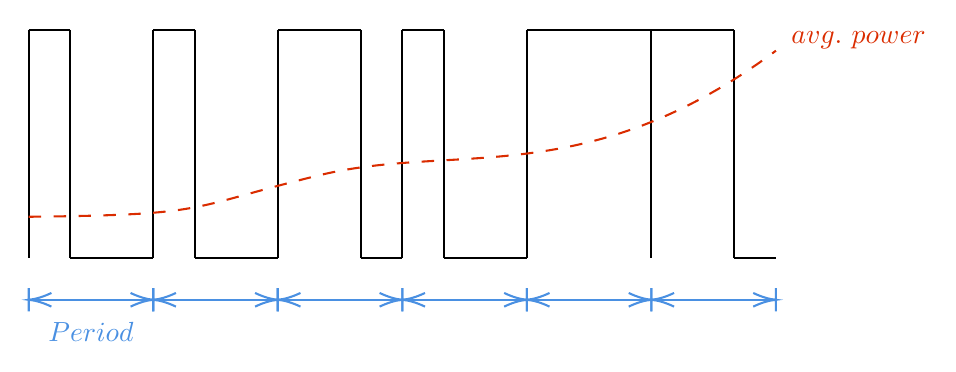
\begin{tikzpicture}[x=0.75pt,y=0.75pt,yscale=-1,xscale=1]
%uncomment if require: \path (0,300); %set diagram left start at 0, and has height of 300

%Straight Lines [id:da37450572503117363] 
\draw    (100,130) -- (120,130) ;
%Straight Lines [id:da7323318640251014] 
\draw    (100,130) -- (100,240) ;
%Straight Lines [id:da1252336596290442] 
\draw    (120,130) -- (120,240) ;
%Straight Lines [id:da3773535073411981] 
\draw    (120,240) -- (160,240) ;
%Straight Lines [id:da20870084265827527] 
\draw    (160,130) -- (180,130) ;
%Straight Lines [id:da2813587021958138] 
\draw    (160,130) -- (160,240) ;
%Straight Lines [id:da509428294567959] 
\draw    (180,130) -- (180,240) ;
%Straight Lines [id:da3684360907767923] 
\draw    (180,240) -- (220,240) ;
%Straight Lines [id:da8436273762111676] 
\draw    (220,130) -- (260,130) ;
%Straight Lines [id:da21845202617269166] 
\draw    (220,130) -- (220,240) ;
%Straight Lines [id:da4633918827590262] 
\draw    (260,130) -- (260,240) ;
%Straight Lines [id:da8964845880277049] 
\draw    (260,240) -- (280,240) ;
%Straight Lines [id:da2005707870676403] 
\draw    (280,130) -- (300,130) ;
%Straight Lines [id:da12573232900267373] 
\draw    (280,130) -- (280,240) ;
%Straight Lines [id:da4554511501371119] 
\draw    (300,130) -- (300,240) ;
%Straight Lines [id:da0740745338558565] 
\draw    (300,240) -- (340,240) ;
%Straight Lines [id:da5383836956811012] 
\draw    (340,130) -- (400,130) ;
%Straight Lines [id:da030754226447927135] 
\draw    (340,130) -- (340,240) ;
%Straight Lines [id:da28147089210249054] 
\draw    (400,130) -- (400,240) ;
%Straight Lines [id:da8364533675885975] 
\draw    (400,130) -- (440,130) ;
%Straight Lines [id:da653074338830008] 
\draw    (400,130) -- (400,240) ;
%Straight Lines [id:da21222926404491116] 
\draw    (440,130) -- (440,240) ;
%Straight Lines [id:da43469497724497785] 
\draw    (440,240) -- (460,240) ;
%Straight Lines [id:da27909048307495965] 
\draw [color={rgb, 255:red, 74; green, 144; blue, 226 }  ,draw opacity=1 ]   (100,260) -- (160,260) ;
\draw [shift={(160,260)}, rotate = 180] [color={rgb, 255:red, 74; green, 144; blue, 226 }  ,draw opacity=1 ][line width=0.75]    (0,5.59) -- (0,-5.59)(10.93,-3.29) .. controls (6.95,-1.4) and (3.31,-0.3) .. (0,0) .. controls (3.31,0.3) and (6.95,1.4) .. (10.93,3.29)   ;
\draw [shift={(100,260)}, rotate = 0] [color={rgb, 255:red, 74; green, 144; blue, 226 }  ,draw opacity=1 ][line width=0.75]    (0,5.59) -- (0,-5.59)(10.93,-3.29) .. controls (6.95,-1.4) and (3.31,-0.3) .. (0,0) .. controls (3.31,0.3) and (6.95,1.4) .. (10.93,3.29)   ;
%Straight Lines [id:da5933914723976027] 
\draw [color={rgb, 255:red, 74; green, 144; blue, 226 }  ,draw opacity=1 ]   (160,260) -- (220,260) ;
\draw [shift={(220,260)}, rotate = 180] [color={rgb, 255:red, 74; green, 144; blue, 226 }  ,draw opacity=1 ][line width=0.75]    (0,5.59) -- (0,-5.59)(10.93,-3.29) .. controls (6.95,-1.4) and (3.31,-0.3) .. (0,0) .. controls (3.31,0.3) and (6.95,1.4) .. (10.93,3.29)   ;
\draw [shift={(160,260)}, rotate = 0] [color={rgb, 255:red, 74; green, 144; blue, 226 }  ,draw opacity=1 ][line width=0.75]    (0,5.59) -- (0,-5.59)(10.93,-3.29) .. controls (6.95,-1.4) and (3.31,-0.3) .. (0,0) .. controls (3.31,0.3) and (6.95,1.4) .. (10.93,3.29)   ;
%Straight Lines [id:da7253500193703607] 
\draw [color={rgb, 255:red, 74; green, 144; blue, 226 }  ,draw opacity=1 ]   (220,260) -- (280,260) ;
\draw [shift={(280,260)}, rotate = 180] [color={rgb, 255:red, 74; green, 144; blue, 226 }  ,draw opacity=1 ][line width=0.75]    (0,5.59) -- (0,-5.59)(10.93,-3.29) .. controls (6.95,-1.4) and (3.31,-0.3) .. (0,0) .. controls (3.31,0.3) and (6.95,1.4) .. (10.93,3.29)   ;
\draw [shift={(220,260)}, rotate = 0] [color={rgb, 255:red, 74; green, 144; blue, 226 }  ,draw opacity=1 ][line width=0.75]    (0,5.59) -- (0,-5.59)(10.93,-3.29) .. controls (6.95,-1.4) and (3.31,-0.3) .. (0,0) .. controls (3.31,0.3) and (6.95,1.4) .. (10.93,3.29)   ;
%Straight Lines [id:da9542681695033238] 
\draw [color={rgb, 255:red, 74; green, 144; blue, 226 }  ,draw opacity=1 ]   (280,260) -- (340,260) ;
\draw [shift={(340,260)}, rotate = 180] [color={rgb, 255:red, 74; green, 144; blue, 226 }  ,draw opacity=1 ][line width=0.75]    (0,5.59) -- (0,-5.59)(10.93,-3.29) .. controls (6.95,-1.4) and (3.31,-0.3) .. (0,0) .. controls (3.31,0.3) and (6.95,1.4) .. (10.93,3.29)   ;
\draw [shift={(280,260)}, rotate = 0] [color={rgb, 255:red, 74; green, 144; blue, 226 }  ,draw opacity=1 ][line width=0.75]    (0,5.59) -- (0,-5.59)(10.93,-3.29) .. controls (6.95,-1.4) and (3.31,-0.3) .. (0,0) .. controls (3.31,0.3) and (6.95,1.4) .. (10.93,3.29)   ;
%Straight Lines [id:da1514603741651026] 
\draw [color={rgb, 255:red, 74; green, 144; blue, 226 }  ,draw opacity=1 ]   (340,260) -- (400,260) ;
\draw [shift={(400,260)}, rotate = 180] [color={rgb, 255:red, 74; green, 144; blue, 226 }  ,draw opacity=1 ][line width=0.75]    (0,5.59) -- (0,-5.59)(10.93,-3.29) .. controls (6.95,-1.4) and (3.31,-0.3) .. (0,0) .. controls (3.31,0.3) and (6.95,1.4) .. (10.93,3.29)   ;
\draw [shift={(340,260)}, rotate = 0] [color={rgb, 255:red, 74; green, 144; blue, 226 }  ,draw opacity=1 ][line width=0.75]    (0,5.59) -- (0,-5.59)(10.93,-3.29) .. controls (6.95,-1.4) and (3.31,-0.3) .. (0,0) .. controls (3.31,0.3) and (6.95,1.4) .. (10.93,3.29)   ;
%Straight Lines [id:da7494645599136815] 
\draw [color={rgb, 255:red, 74; green, 144; blue, 226 }  ,draw opacity=1 ]   (400,260) -- (460,260) ;
\draw [shift={(460,260)}, rotate = 180] [color={rgb, 255:red, 74; green, 144; blue, 226 }  ,draw opacity=1 ][line width=0.75]    (0,5.59) -- (0,-5.59)(10.93,-3.29) .. controls (6.95,-1.4) and (3.31,-0.3) .. (0,0) .. controls (3.31,0.3) and (6.95,1.4) .. (10.93,3.29)   ;
\draw [shift={(400,260)}, rotate = 0] [color={rgb, 255:red, 74; green, 144; blue, 226 }  ,draw opacity=1 ][line width=0.75]    (0,5.59) -- (0,-5.59)(10.93,-3.29) .. controls (6.95,-1.4) and (3.31,-0.3) .. (0,0) .. controls (3.31,0.3) and (6.95,1.4) .. (10.93,3.29)   ;
%Curve Lines [id:da09794532071820783] 
\draw [color={rgb, 255:red, 218; green, 44; blue, 0 }  ,draw opacity=1 ] [dash pattern={on 4.5pt off 4.5pt}]  (100,220) .. controls (189.23,219.05) and (174.77,215.95) .. (240,200) .. controls (305.23,184.05) and (368.23,208.05) .. (460,140) ;

% Text Node
\draw (130,269.4) node [anchor=north] [inner sep=0.75pt]  [color={rgb, 255:red, 74; green, 144; blue, 226 }  ,opacity=1 ]  {$Period$};
% Text Node
\draw (466,129.4) node [anchor=north west][inner sep=0.75pt]  [color={rgb, 255:red, 218; green, 44; blue, 0 }  ,opacity=1 ]  {$avg.\ power$};

\end{tikzpicture}

    \caption{Pulse Width Modulation Visual}
    \label{fig:pwm}
\end{figure}
\subsection{DC Motor Modeling}
Motor modeling is one major challenge when creating a system for control. Quite often, cheap motors will not have a datasheet associated with them and the motor parameters and modeling must be figured out by the end-user. Luckily, many of these important parameters can be experimentally determined and estimated to an acceptable level of precision. Here, I will discuss three main types of controllers for the DC motor. These are:
\begin{enumerate}
    \item Position Control
    \item Speed Control
    \item Torque Control
\end{enumerate}
Many textbooks discuss information on position and speed control, but little is said of torque control! Torque control is actually quite important in our application with the inverted pendulum, since our input is a force! It is necessary to understand the torque output of the motor in our modeling for adequate control of the system.

\subsubsection{Motor Modeling from first principles}
The DC motor can fundamentally be understood as a circuit. Here, the properties of the magnetic field and the internal nature of the DC motor are not considered. There are many sources, such as \cite{golnaraghi_automatic_2017,evans_dc_2020,sabin_civil_engineering_dc_2014} which describe the mechanical design and electromagnetic effects of the DC motor. The circuit of the DC motor is quite simple and is shown in \autoref{fig:dc motor circuit}.

\begin{figure}[ht]
    \centering

\begin{tikzpicture}
	% Paths, nodes and wires:
	\node[shape=rectangle, draw, line width=1pt, inner sep=0, minimum width=0.318cm, minimum height=0.288cm](Rect1) at (6, 2.93){} node[anchor=south east] at ([xshift=-0.12cm, yshift=0.12cm]Rect1.west){$+$};
	\draw (1, 4) to[american voltage source, l_={$V$}, label distance=0.02cm] (1, 1);
	\node[shape=rectangle, draw, line width=1pt, inner sep=0, minimum width=0.318cm, minimum height=0.288cm](Rect2) at (6, 2.07){} node[anchor=north east] at ([xshift=-0.12cm, yshift=-0.12cm]Rect2.west){$-$};
	\node[shape=circle, fill={rgb,255:red,255;green,255;blue,255}, draw, line width=1pt, inner sep=0, minimum width=0.825cm](Ellipse1) at (6, 2.5){} node[anchor=east] at ([xshift=-0.12cm]Ellipse1.west){$e=k_e\omega$};
	\draw (6, 4) -| (6, 3.092);
	\draw (6, 1.908) -| (6, 1);
	\draw (6, 1) |- (1, 1);
	\draw (1, 4) to[american resistor, l={$R$}, label distance=0.02cm] (3.5, 4);
	\draw (3.5, 4) to[cute inductor, l={$L$}, label distance=0.02cm] (6, 4);
	\draw[-latex] (3, 4.5) -- (4, 4.5);
	\node[shape=rectangle, inner sep=0, minimum width=0.965cm, minimum height=0.465cm](Rect3) at (3.5, 4.75){} node[anchor=center] at (Rect3.center){$i$};
\end{tikzpicture}
    
    \caption{DC Motor Circuit}
    \label{fig:dc motor circuit}
\end{figure}
This diagram shows the basic operation of the motor, but is adequate to create a model that works quite well and has been shown to agree with real motor dynamics. In this model, $V$ is the voltage of the power source, $R$ is the motor resistance, $L$ is the inductance, $i$ is the current, and $e$ is the back-emf of the motor.

We will begin with by modeling the dynamics of the electrical system, which we may further build upon with the mechanical system dynamics. To construct differential equations for this circuit, we can employ Kirchhoff's Law such that $\sum V=0$.
$$V-iR-L\frac{di}{dt}-e=0$$
The back-emf of the motor is a function of the rotational speed of the motor, $\omega$, multiplied by a constant value $k_e$.
$$V=iR+L\frac{di}{dt}+k_e\omega$$
This is the governing differential equation of the electric circuit of the DC motor, which is a first order differential equation. We can convert this equation to the Laplace domain to develop a transfer function for the system:
$$V(s) = (R+Ls)I(s)+k_e\omega(s)$$

\subsubsection{Dynamics Modeling}
Dynamics modeling is quite simple for the DC motor, as we need only consider that:
$$\sum\tau=J\dot{\omega}$$
Note that the typical use of $I$ for the moment of inertia here has been replaced with $J$ since $I$ is being used for current. The torque balance is given by taking the motor output torque, and subtracting the friction and disturbance torques on the system:
$$\tau-b\omega-\tau_d=J\dot{\omega}$$
Once again, this relationship can be rewritten in the Laplace domain:
$$\tau(s)-b\omega(s)-\tau_d=Js\omega(s)$$

\subsubsection{Speed Control}

\subsubsection{Velocity Control}

\subsubsection{Torque Control}
The DC motor operates through the generation of a magnetic field and a current carrying conductor in the motor. The torque that is generated by a motor is a result of the Lorentz force. The interaction of these magnetic fields and electric currents induces a torque:
$$\tau=k_ii$$
And as the motor increases in speed there is a voltage produced which resists motion due to Lenz' Law:
$$e=K\phi\omega$$

When we use SI units, it turns out that $k_i$ and $k_m$ have different units, but are the exact same value. We can therefore replace these with the single motor constant, $k$.


Finally, we arrive at the transfer function which relates torque and voltage.
$$\frac{\tau(s)}{V(s)}=\frac{k_i(Js+b)}{(Js+b)(Ls+R)+k_ik_m}$$



\subsection{Motor Control Algorithms}
No matter what type of motor is selected for use, a control algorithm must be developed for the control of the motor itself, separate from the control of the overall system. The action of the motor controller is to match the desired RPM, position, or torque of the system quickly and accurately to facilitate good control of the system. At a high level, the control system for a DC motor will look like \autoref{fig:dc motor controller}:

\begin{figure}
    \centering


\tikzset{every picture/.style={line width=0.75pt}} %set default line width to 0.75pt        

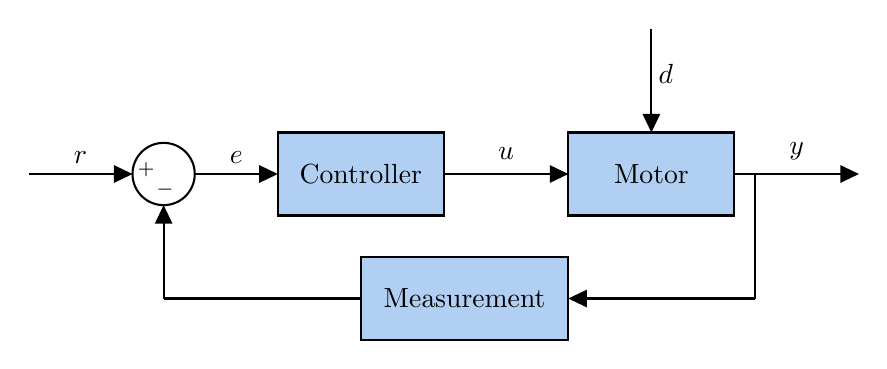
\begin{tikzpicture}[x=0.75pt,y=0.75pt,yscale=-1,xscale=1]
%uncomment if require: \path (0,300); %set diagram left start at 0, and has height of 300

%Flowchart: Process [id:dp4083062669705493] 
\draw  [fill={rgb, 255:red, 74; green, 144; blue, 226 }  ,fill opacity=0.43 ] (220,130) -- (300,130) -- (300,170) -- (220,170) -- cycle ;
%Flowchart: Process [id:dp7176923014407074] 
\draw  [fill={rgb, 255:red, 74; green, 144; blue, 226 }  ,fill opacity=0.43 ] (360,130) -- (440,130) -- (440,170) -- (360,170) -- cycle ;
%Straight Lines [id:da7872115144137771] 
\draw    (300,150) -- (357,150) ;
\draw [shift={(360,150)}, rotate = 180] [fill={rgb, 255:red, 0; green, 0; blue, 0 }  ][line width=0.08]  [draw opacity=0] (8.93,-4.29) -- (0,0) -- (8.93,4.29) -- cycle    ;
%Straight Lines [id:da6962065446356057] 
\draw    (440,150) -- (497,150) ;
\draw [shift={(500,150)}, rotate = 180] [fill={rgb, 255:red, 0; green, 0; blue, 0 }  ][line width=0.08]  [draw opacity=0] (8.93,-4.29) -- (0,0) -- (8.93,4.29) -- cycle    ;
%Straight Lines [id:da7394890428771211] 
\draw    (100,150) -- (147,150) ;
\draw [shift={(150,150)}, rotate = 180] [fill={rgb, 255:red, 0; green, 0; blue, 0 }  ][line width=0.08]  [draw opacity=0] (8.93,-4.29) -- (0,0) -- (8.93,4.29) -- cycle    ;
%Flowchart: Process [id:dp8311908981055321] 
\draw  [fill={rgb, 255:red, 74; green, 144; blue, 226 }  ,fill opacity=0.43 ] (260,190) -- (360,190) -- (360,230) -- (260,230) -- cycle ;
%Straight Lines [id:da799256410638905] 
\draw    (450,150) -- (450,210) ;
%Straight Lines [id:da3431019163397425] 
\draw    (450,210) -- (363,210) ;
\draw [shift={(360,210)}, rotate = 360] [fill={rgb, 255:red, 0; green, 0; blue, 0 }  ][line width=0.08]  [draw opacity=0] (8.93,-4.29) -- (0,0) -- (8.93,4.29) -- cycle    ;
%Shape: Circle [id:dp2745941889127239] 
\draw   (150,150) .. controls (150,141.72) and (156.72,135) .. (165,135) .. controls (173.28,135) and (180,141.72) .. (180,150) .. controls (180,158.28) and (173.28,165) .. (165,165) .. controls (156.72,165) and (150,158.28) .. (150,150) -- cycle ;
%Straight Lines [id:da517382267392099] 
\draw    (165,210) -- (165,168) ;
\draw [shift={(165,165)}, rotate = 90] [fill={rgb, 255:red, 0; green, 0; blue, 0 }  ][line width=0.08]  [draw opacity=0] (8.93,-4.29) -- (0,0) -- (8.93,4.29) -- cycle    ;
%Straight Lines [id:da24863642236992634] 
\draw    (165,210) -- (260,210) ;
%Straight Lines [id:da7137782715695976] 
\draw    (180,150) -- (217,150) ;
\draw [shift={(220,150)}, rotate = 180] [fill={rgb, 255:red, 0; green, 0; blue, 0 }  ][line width=0.08]  [draw opacity=0] (8.93,-4.29) -- (0,0) -- (8.93,4.29) -- cycle    ;
%Straight Lines [id:da9418326504220698] 
\draw    (400,80) -- (400,127) ;
\draw [shift={(400,130)}, rotate = 270] [fill={rgb, 255:red, 0; green, 0; blue, 0 }  ][line width=0.08]  [draw opacity=0] (8.93,-4.29) -- (0,0) -- (8.93,4.29) -- cycle    ;

% Text Node
\draw (260,150) node   [align=left] {Controller};
% Text Node
\draw (400,150) node   [align=left] {Motor};
% Text Node
\draw (125,146.6) node [anchor=south] [inner sep=0.75pt]    {$r$};
% Text Node
\draw (330,144.6) node [anchor=south] [inner sep=0.75pt]    {$u$};
% Text Node
\draw (470,144.6) node [anchor=south] [inner sep=0.75pt]    {$y$};
% Text Node
\draw (310,210) node   [align=left] {Measurement};
% Text Node
\draw (151,148) node [anchor=west] [inner sep=0.75pt]  [font=\scriptsize]  {$+$};
% Text Node
\draw (160,157.5) node [anchor=west] [inner sep=0.75pt]  [font=\scriptsize]  {$-$};
% Text Node
\draw (402,102) node [anchor=west] [inner sep=0.75pt]    {$d$};
% Text Node
\draw (200,146.6) node [anchor=south] [inner sep=0.75pt]    {$e$};

\end{tikzpicture}

    \caption{High level DC motor control system}
    \label{fig:dc motor controller}
\end{figure}

For DC motor control, \gls{pid} controllers are quite common. Other control algorithms may be implemented, such as \gls{lqr} or \gls{lqi}, but their implementation has been discussed elsewhere in this text quite thoroughly. \Gls{pid} control is quite popular in such applications for it's widespread use, easy tunability, and simple application in the time-domain.  Because the motor transfer functions are \gls{siso}, \gls{pid} is quite well suited for this application. For this reason, this section will detail the implementation of \gls{pid} for these motor controllers in several applications.

Here, I will detail the various methods by which \gls{pid} gains can be attained. An emphasis is placed on the \gls{pid} control of motor systems. More than anything, this is to give a taste of what can be done for such a system, and is not representative of the full scope of choices that can be made. Each control system will have its own challenges that must be overcome! 

\subsubsection{PID Gain Methods}
There are several approaches which can be used to arrive at appropriate \gls{pid} gains for the system. These vary in complexity and the application of one approach over the other will depend on the system. At the most basic level, the \gls{pid} gains can be achieved experimentally without modeling of the system dynamics using methods such as Ziegler-Nichols and Cohen-Coon methods. There approaches are heuristic in nature in that they select \gls{pid} gains which have been shown to work in experiments and are a good rule of thumb.

Beyond this, modeling of the system dynamics is required for further analysis. System dynamics can be derived in several ways, either starting from first principles of the system or from equations which are known to describe DC motor dynamics. Further still, approaches exist to experimentally determine the transfer function and frequency response of a system and use this as a model. All of these approaches are valid. In this section, all of these approaches will be considered and shown to yield similar results.

\subsubsection{ZN and Cohen-Coon PID Methods}
I will start this section by considering the simplest methods of \gls{pid} tuning. For many systems, such methods are perfectly fine and are quite practical. As will be seen, using these methods yields a perfectly usable \gls{pid}.

The Zeigler-Nichols methods and the Cohen-Coon methods are methods that find the gains of the system through simple equation relations. The relationships for the Ziegler-Nichols Method are given in \autoref{tab:ZN tuning}.

\begin{table}[ht]
\centering
\caption{Ziegler–Nichols Method Tuning Parameters}
\begin{tabular}{@{}lccc@{}}
\toprule
\textbf{Control Type} & \( K_p \) & \( K_i \) & \( K_d \) \\
\midrule
P & \( 0.5K_u \) & -- & -- \\
PI & \( 0.45K_u \) & \( 0.54K_u / T_u \) & -- \\
PD & \( 0.8K_u \) & -- & \( 0.10K_u T_u \) \\
Classic PID & \( 0.6K_u \) & \( 1.2K_u / T_u \) & \( 0.075K_u T_u \) \\
Pessen Integral Rule & \( 0.7K_u \) & \( 1.75K_u / T_u \) & \( 0.105K_u T_u \) \\
Some Overshoot & \( 0.33\overline{K}_u \) & \( 0.66K_u / T_u \) & \( 0.11K_u T_u \) \\
No Overshoot & \( 0.20K_u \) & \( 0.40K_u / T_u \) & \( 0.066K_u T_u \) \\
\bottomrule
\end{tabular}
\label{tab:ZN tuning}

\end{table}
In the ZN tuning method, a steady state value is commanded with a controller with only proportional gain, P. The gain is slowly increased at this steady state condition until oscillations about the steady state condition begin to appear. The gain at which this occurs is the gain $K_u$. The frequency of the oscillation is $T_u$.

After these values are determined, the table is then used to determine appropriate \gls{pid} gains based on the type of controller and the desired system behavior. 

\begin{example}[ZN Tuning of DC motor]

    
\end{example}

\subsubsection{Encoder Modeling}
Encoders are devices that measure the linear or rotational motion. Incremental encoders, which measure `ticks' of a rotation or movement are the most common type are are employed on the inverted pendulum for capturing the true speed of the motor, as well as it's position.

Since a DC motor may rotate in either direction, it is impossible to tell the direction of rotation with a single measurement. There is no possible distinction between forward and backward rotation simply by measuring the number of clicks. For this reason, most encoders employ two channels. These sensors are often placed $90\degree$ apart which results in a quadrature layout. In this type of layout, there are 4 pulses which are sent for each cycle.

\begin{example}[RPM measurement from encoder output]
    To determine the RPM of a motor from encoder reading outputs, we first need to determine the number of pulses that are sent for each revolution of the motor. This number of \gls{ppr} of the encoder should be included in the datasheet of the encoder. If it is not, it is possible to determine this value by setting a fixed RPM (say 60 RPM) and changing the value of the \gls{ppr} until the shaft rotates at a true 60 RPM. When the motor is using quadrature encoding, the value of the \gls{ppr} may need to be multiplied by 4.

    Consider a motor with a 18.8x gear reduction and an encoder with 16 \gls{ppr} with quadrature encoding. The pulses of the encoder are measured at $100 \ \mathrm{Hz}$. We can derive the RPM of the motor through the following formula:
$$\frac{\mathrm{\# \ pulses}}{4\cdot18.8\cdot\mathrm{PPR}} \cdot \frac{60}{\Delta t}$$
The value for the quadrature encoding and the motor gear ratio can be included in the value of the \gls{ppr} if desired.
\end{example}

\section{Simulation}\label{sec:sim}
After we have developed appropriate models for all of the subsystems, full simulation of the system can allow us to validate these models and improve the control algorithm. 

The core of the simulation is based on the non-linear dynamics which have been derived in \autoref{sec:pend eom}. All we need to do is to reduce these equations into a system of first order \glspl{ode}. The original equations of motion from \eqautoref{eq:inverted pend eom} have been reproduced here for convenience:
\begin{gather}
\begin{array}{c}
     (M+m)\ddot{x}+ml\cos\theta\ddot{\theta}-ml\sin\theta\dot{\theta}^2=F \\I\ddot{\theta}+ml\cos\theta\ddot{x}-mgl\sin\theta=0
\end{array}
\end{gather}
Following the standard method of reduction, these equations are turned into:
\begin{gather}
    \dot{x}=v\\
    \dot{\theta}=\omega\\
         (M+m)\dot{v}+ml\cos\theta\dot{\omega}-ml\sin\theta\omega^2=F \\I\dot{\omega}+ml\cos\theta\dot{v}-mgl\sin\theta=0
\end{gather}

\section{Real Implementation}
To begin the discussion of the real implementation of the inverted pendulum, we must discuss the hardware used, as that directly ties into how we build our state space model and what assumptions that we can use in the design.

I should note that I am presenting this \textit{after} presenting the theory of the system, but in practice, these are often developed alongside each other. The hardware will dictate some facts about the control system, especially under certain budget, size, and power constraints.

On the converse, simulation and theory will provide some other constraints for the system. In practice, there is no clear distinction between a `simulation' phase of the design and a `building' phase. It is often the case with control systems that they inform each other and are very tightly coupled. 

\subsection{Physical Design}
The physical design of the pendulum is quite important to understand which dynamical phenomena are important for our modeling. Additionally, the physical components will dictate features of the system observability and place limitations on the control scheme. A technical drawing of the pendulum is shown in \autoref{fig:pend schem}.

\begin{figure}[H]
    \centering
    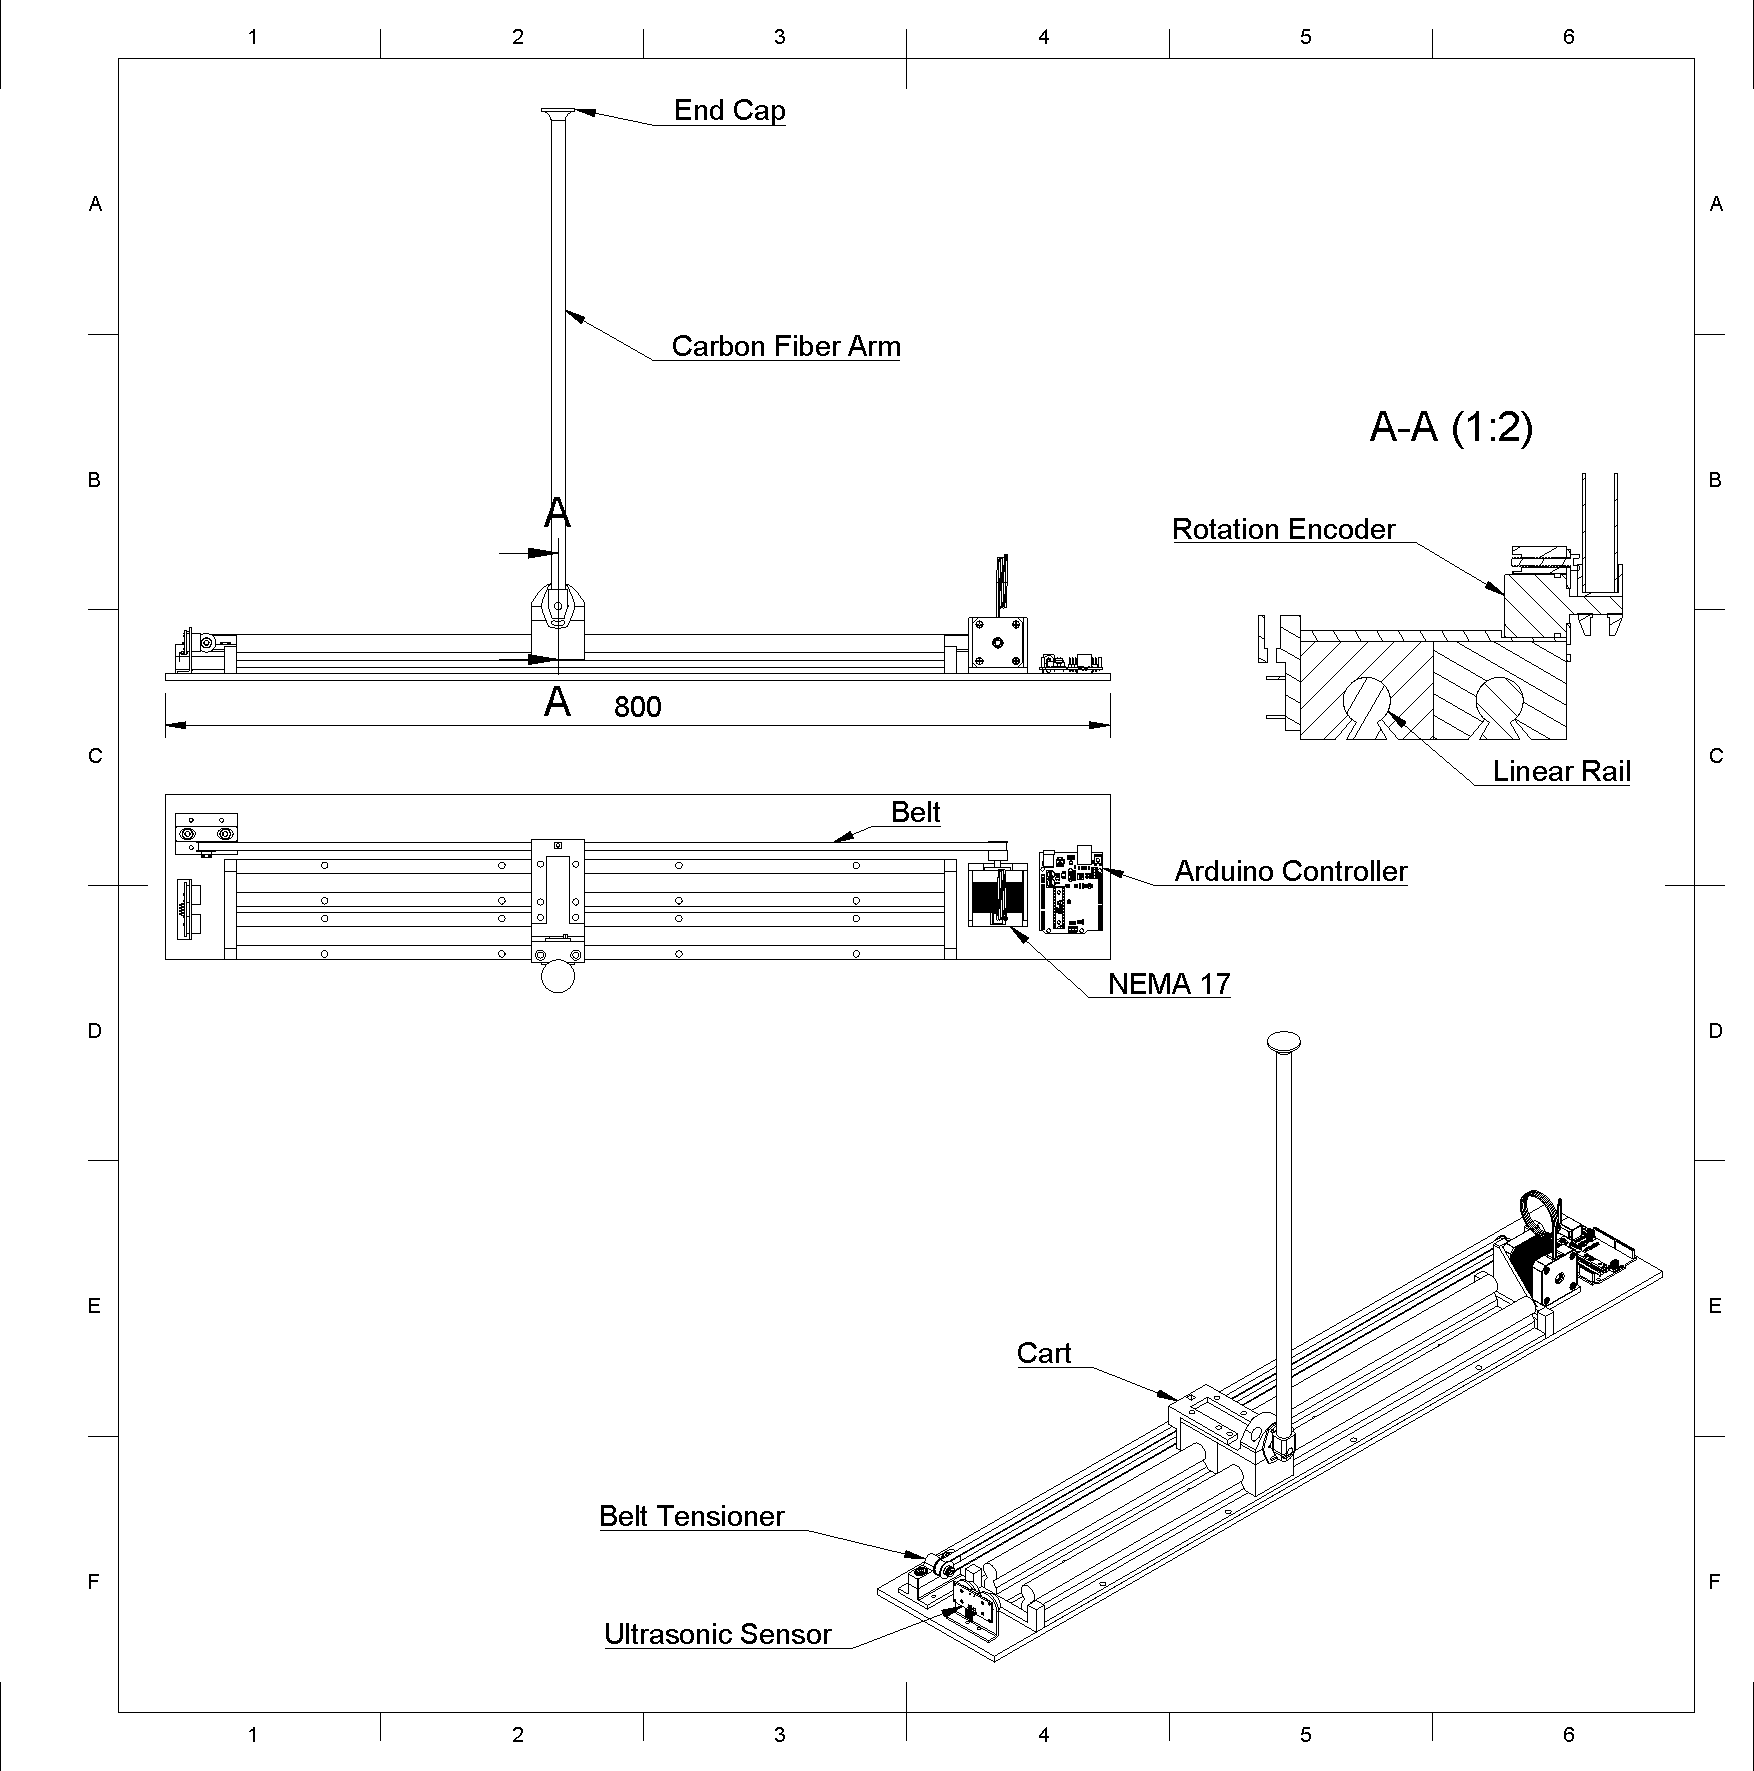
\includegraphics[width=\linewidth]{Images/InvertedPendulumSchematic.pdf}
    \caption{Inverted Pendulum Schematic}
    \label{fig:pend schem}
\end{figure}
A breakdown of the components in the pendulum is done below, considering both the electronics and mechanical systems which will inform the control system design.

\subsubsection{Mechanical Considerations}
The mechanics of the inverted pendulum and cart are fairly simple. The main consideration is the selection of the length of the rails, and ensuring that the friction and mass of the cart are as low as possible. In this design, rails of the SBR16 specification were selected, although many other types of rail systems may be used. Some other types of linear rails and bearings may permit a lower mass cart, which is desirable.

Another important criteria is the selection of the belt drive and pulley system, which will dictate the conversion between RPM and linear speed for the system. A larger diameter pulley will result in higher linear speeds for a given RPM, but will also require more torque. The belt drive system here uses a GT2 belt with 20 tooth pulleys. Other pulley diameters may be used if more precise control or higher speed output is desirable for the given application.

\subsubsection{Rotary Encoder}
In cross section A-A, the rotary encoder can be seen. The rotary encoder is one of the most important components in the design as the angle measurement of the arm is very important in understanding the dynamics of the system. The particular model used here can be found at \cite{noauthor_yuecoom_nodate}.

This rotary encoder is a hall effect sensor, so it is contactless. The sensor has 12-bit precision and can measure angles to a precision of $0.088\degree$ as a result. This type of sensor has much less sensor noise than a common potentiometer and also produces less resistance to rotation. This reduction in drag helps the pendulum arm rotate more freely. For this project, I have mounted the pendulum arm directly onto the end of the sensor. However, for heavier loads, it may be wise to place the load on a bearing instead of the sensor itself.

Another important feature of the rotary encoder is the sensor linearity. For this model, the sensor linearity is 0.3\% of the full scale, which means that the maximum deviation from the true output is less than 0.3\% of $360\degree$, or less than $1.08\degree$.

\subsubsection{Arm}
The design of the physical arm is also quite important to the development of a control model for the pendulum. For a pendulum undergoing small oscillations, the period is given by 
$$T=2\pi\sqrt{\frac{l}{g}}$$
From this relation, we can see that increasing the length will increase the period and make the system easier to control. Of course, this is quite different for the inverted case since the fixed point is unstable. However, this still gives a heuristic for how long the pendulum will take to fall.

If we want to be more precise, we may take the linear equations of motion in \eqautoref{eq:linear pend} and assume that the acceleration $\ddot{x}$ is 0:
$$I\ddot{\theta}=mgl\theta$$
The exact moment of inertia of the system may change, but the moment of inertia must always have units of $ml^2$. If we let $I=Cml^2$, then:
$$\ddot{\theta}=\frac{g}{Cl}\theta$$
We can see that for small angles, the acceleration of the pendulum away from the equilibrium position is inversely related to the length of the pendulum and the moment of inertia, $C$. For this reason, it is quite easy to balance a broom vertically, but balancing a pencil is almost impossible!

For our system then, we should choose values that make controlling the system possible without extraordinarily fast electronics or microcontrollers. At the same time, the arm should be easily carried around and not so large as to require a huge motor to move it. A length of around $0.5\ \mathrm{m}$ is a good compromise between the two. Assuming the arm has a moment of inertia that is the same as a thin rod, $\frac{1}{3}ml^2$, then the acceleration is around $6.3 \ \mathrm{rad/s^2}$ for an angle of  $5\degree$. After this point, nonlinear effects become quite prevalent and the analysis breaks down. Of course, smaller angles will exhibit rotational accelerations which are smaller in direct linear relation with the angle.

For further investigation, we can consider the linear acceleration that would be required to restore $\ddot{\theta}$ to 0 as a first approximation of the required linear acceleration required of the system. This can be done using \eqautoref{eq:theta double dot pend} and plugging in $\ddot{\theta}$ as $6.3 \ \mathrm{rad/s}$ and $\theta$ as $5\degree$:
$$\ddot{x}=l\ddot\theta-g\theta\approx1.72 \ \mathrm{m/s^2}$$
We can think of these conditions as a worst possible case, where the cart needs to accelerate rapidly to compensate for a large angular error. Ideally, the control system will maintain an angle less that $5\degree$. In this case, the system needs to have the capability of acceleration up to $1.72 \ \mathrm{m/s^2}$.

While this analysis is non-perfect, it is at least a good heuristic for selecting an appropriate arm length for the pendulum. For further analysis of non-linear dynamics, simulation is often a good idea. Computing the non-linear dynamics using MATLAB/Simulink and providing the control algorithm can give a good idea of the amount of acceleration, peak velocity, and torque the system will need. All of these will be crucial to the selection of motor for the project. The set up of such a simulation has been described in \autoref{sec:sim}.
\subsection{Noise and Data Dropouts}
Noisy data is quite common in real world sensors, especially those found in low cost electronics. This is especially prevalent when the derivative of a signal must be computed. One repercussion of computing the derivative of a signal is that high frequency components of the signal (where most of the noise resides) are amplified.\endnote{This can be seen by considering a signal that is decomposed into its Fourier series:
$$f(t)=\sum_{k=-\infty}^{\infty}a_ke^{ik\omega_0t}$$
Taking the time derivative of the signal yields:
$$\frac{df(t)}{dt}=i\omega_0\sum_{k=-\infty}^{\infty}ka_ke^{ik\omega_0t}$$
Application of Parseval's formula gives that:
$$\frac{1}{\tau}\int_0^\tau\left|\frac{df(t)}{dt}\right|^2dt={\omega_0}^2\sum_{k=-\infty}^{\infty}|ka_k|^2$$
Which makes it evident that the power in the higher frequencies of the signal has been amplified as compared to the original signal} 

Another problem that occurs with real world signals is data dropouts. Dropouts can be quite common for some sensors, such as the encoders of DC motors. One way to deal with data dropouts is to include some logic that checks the difference in the signal output. If the difference is greater than some expected threshold, the data is disregarded. An example of such a code for implementation into MATLAB or Simulink is shown below:
\begin{lstlisting}[style=Matlab-editor]
function filtered = filterEncoder(currVal)

persistent prevVal

% Initialize on first call
if isempty(prevVal)
    prevVal = currVal;
end

% Dropout detection
threshold = 200;  % Adjust based on your system

if abs(currVal - prevVal) > threshold
    % Bad reading: keep previous good value
    filtered = prevVal;
else
    % Good reading: update and pass through
    filtered = currVal;
    prevVal = currVal;
end
\end{lstlisting}

A "persistent" variable is one which maintains its value across multiple function calls. Depending on the type of dropouts, more advanced approaches may need to be taken.

Dealing with noise is often done through the application of a low-pass filter or a moving average filter. These filters induce some delay in the signal, but signal delay is often preferable to noisy data. Either of these filters can be added in Simulink.

\newpage
\printendnotes